\documentclass[11pt]{article}
\usepackage[margin=1in]{geometry}
\usepackage[table]{xcolor}
\usepackage{amsmath,amssymb}
\usepackage{graphicx}
\usepackage{booktabs,multirow,makecell,array}
\usepackage{float}
\usepackage{adjustbox}
\usepackage[font=small]{caption}
\usepackage{enumitem}
\usepackage{pifont}
\usepackage{algorithm}
\usepackage{algpseudocode}
\usepackage{subcaption}
\usepackage{textcomp}
\newcommand{\cmark}{\ding{51}}
\newcommand{\xmark}{\ding{55}}
\providecommand{\balance}{}
\providecommand{\IEEEPARstart}[2]{#1#2}

\renewcommand{\thetable}{\Roman{table}}
\newenvironment{excerpt}{\begin{quote}\sloppy}{\end{quote}}
\newcommand{\review}[2]{\par\bigskip\noindent\textbf{\textit{Review #1}}\ \ \textit{``#2''}\par\smallskip\hrule\medskip}
\newcommand{\reply}{\noindent\textbf{Reply}: }
\newcommand{\mshead}[2]{\subsection*{\textbf{#1. #2}}}
\newcommand{\loc}[1]{\par\medskip\noindent\textbf{#1}\par}
\setlength{\parskip}{4pt}

\begin{document}

\begin{titlepage}
\centering
\vspace*{\fill}
{\Large CONQUEST: A Federated Context-Aware Quantum-Inspired Framework for Robust Cyberworm Detection in Mission-Critical IoT Networks\par}
\vspace{0.6cm}
{\large (Manuscript Number: IoT-64147-2026)\par}
\vspace{0.6cm}
{\large Response to the Associate Editor and Reviewers\par}
\vspace{0.6cm}
{October 2026\par}
\vspace*{\fill}
\end{titlepage}

%% =====================================================================
\section*{To Associate Editor}

Thank you for handling our manuscript and for your remarks. According to
your letter, our paper (IoT-64147-2026) requires mandatory minor revisions
based on the comments of Reviewers 1 and 2. We have revised the manuscript
accordingly. Below, the reviewers' remarks are given in italics, followed by
our reply in regular style. In the revised manuscript, every modification is
highlighted in red; the highlighting remains visible when the file is
printed. Excerpts of the revised manuscript are reproduced below each reply,
starting from the heading of the section or subsection that contains the
change, so that each revision is shown in its context. Within each excerpt,
only the text that answers the comment is shown in red; the surrounding text,
including revisions made for other comments, is shown in black. Page,
section, table, figure, and equation numbers refer to the revised manuscript. Table~A summarizes the major differences between the previous
and the revised manuscript.

\begin{table}[H]
\centering
\caption*{Table A: Summary of major differences between the previous manuscript and the revised version.}
\begin{tabular}{lcc}
\toprule
Paper changes & Previous manuscript & Revised manuscript \\
\midrule
Number of pages & 16 & 20 \\
Number of figures & 7 & 10 \\
Number of tables & 9 & 17 \\
Number of algorithms & 0 & 1 \\
Number of references & 35 & 42 \\
\bottomrule
\end{tabular}
\end{table}

To answer the comments, all experiments were repeated under a single,
leakage-free protocol: a blocked temporal split in which every fitting,
selection, and stopping step uses the training or validation data only, ten
seeds per centralized configuration with QPSO re-executed in every run, and
one common configuration for all federated experiments. The main changes are:
\begin{itemize}[leftmargin=*,itemsep=1pt]
  \item an exact definition of how the register size $Q$ enters QPSO
        (Eqs.~(7)--(11), Algorithm~1, Table~V) and an analysis of the search
        dynamics versus $Q$ (Fig.~3);
  \item a ten-seed register-size ablation with Friedman and Holm-corrected
        Wilcoxon tests, a search-budget sensitivity study, and the selected
        feature subset with its stability across seeds;
  \item a $2\times2$ factorial ablation of context features and QPSO, and a
        classical PSO baseline at an equal search budget;
  \item exact definitions of the 17 context features and a table of the data
        used by every fitting, selection, and stopping step;
  \item a federated evaluation under one configuration with $K=5$, 10, and
        20 clients, three aggregators, three mask-construction modes, a threat
        model, secure aggregation, and differential privacy;
  \item a redefined, separately measured deployment cost with explicit units
        and measurement procedure;
  \item a table that distinguishes the journal extension from the conference
        version.
\end{itemize}

%% =====================================================================
\clearpage
\section*{To Reviewer \#1}

The authors appreciate the reviewer's careful and constructive evaluation.
The comments identified the points where the definition of the method, the
statistical support of its claims, and the reporting of its costs were not
yet sufficient for reproduction. Addressing them has substantially
strengthened the manuscript.

%% ---------------------------------------------------------------------
\review{1.1}{In Section III, manuscript pp.~4--6, particularly Table II and Eqs.~(6)--(9), $Q$ is defined as the `number of qubits,' but its actual role in the QPSO algorithm is unclear. The particle is defined as $p_i \in [0,1]^d$ and the mask as $m_i \in \{0,1\}^d$, while $Q$ does not appear in the update equations. The authors should explicitly define how $Q$ changes the particle representation, search process, and mapping to the feature mask.}

\reply We thank the reviewer for this important comment. Section~III-B now
defines the complete QPSO procedure and states exactly where $Q$ enters it.
\begin{itemize}[leftmargin=*,itemsep=1pt]
  \item \textit{Particle representation.} Each particle holds one
        non-negative, normalized amplitude per feature, so its dimension is
        $d$ for every $Q$; $Q$ does not change the representation.
  \item \textit{Search process.} $Q$ enters at three points: the
        initialization at the uniform amplitude of a $Q$-qubit register
        (Eq.~(7)), the rotation-angle bound $\pi/(2Q)$ toward the personal and
        global bests (Eqs.~(8)--(9)), and the collapse probability $2^{-Q}$
        with which each amplitude is reset (Eq.~(10)). Algorithm~1 marks these
        steps, and Table~V lists the resulting constants for $Q=1$ to 10.
  \item \textit{Mapping to the mask.} A mask is obtained by drawing $k$
        distinct features with probabilities proportional to the squared
        amplitudes (Eq.~(11)); each run returns the highest-fitness mask
        evaluated. $k$ is fixed, so $Q$ determines which features are found,
        not how many.
\end{itemize}
Fig.~3 confirms the resulting behavior empirically: $Q=1$ samples almost
uniformly, $Q=4$ to 7 concentrate the search on a feature subset, and
$Q\ge9$ barely moves the particles. The notation table (Table~III) now
defines $Q$, $d$, $k$, $P$, and $I$, and the manuscript states that the
method is quantum-inspired and simulates no quantum state.

\loc{(a) Page 6: Added the particle representation, the role of $Q$, and the mask measurement to Section III-B}
\begin{excerpt}
\mshead{III-B}{Variable-Qubit QPSO Feature Selection}


QPSO learns a sparse binary feature mask
$\mathbf{m}\in\{0,1\}^d$ that gates the normalized input:
\begin{equation}
\tilde{\mathbf{z}} = \mathbf{m}\odot\mathbf{z}_n,\quad
\|\mathbf{m}\|_0 = k \ll d,
\tag{6}
\end{equation}
where $\odot$ denotes element-wise multiplication.
\textcolor{red}{Each of the $P$ particles $i$ holds a
non-negative amplitude vector $\mathbf{a}_i\in\mathbb{R}_{\ge 0}^{d}$
with $\sum_j a_{i,j}=1$, one amplitude per feature, so the particle
dimension is $d$ for every $Q$. The register size $Q$ enters the
search at three points. First, amplitudes are initialized at the
uniform amplitude of a $Q$-qubit register plus Gaussian noise; after
normalization, only the relative perturbation
$\rho(Q)=2^{Q/2}/(Q^{2}+1)$ matters:}
\begin{equation}
\textcolor{red}{a_{i,j}^{(0)} \propto \Bigl|\,2^{-Q/2} +
\tfrac{\xi_{i,j}}{Q^{2}+1}\Bigr|,\quad
\xi_{i,j}\sim\mathcal{N}(0,1).}
\tag{7}
\end{equation}
\textcolor{red}{Second, at iteration $t$, each particle is
rotated toward its personal-best amplitude $\mathbf{a}_i^{\rm pb}$
and the global-best amplitude $\mathbf{a}^{\rm gb}$ by an angle whose
upper bound decreases with $Q$:}
\begin{align}
\textcolor{red}{\phi_t} &\textcolor{red}{= \frac{\pi}{2Q}\Bigl(1-\frac{t}{I}\Bigr),}
\tag{8}\\
\textcolor{red}{\mathbf{a}_i} &\textcolor{red}{\leftarrow \mathbf{a}_i
+ r_1\cos\phi_t\,(\mathbf{a}_i^{\rm pb}-\mathbf{a}_i)
+ r_2\sin\phi_t\,(\mathbf{a}^{\rm gb}-\mathbf{a}_i),}
\tag{9}
\end{align}
\textcolor{red}{with $r_1,r_2\sim\mathcal{U}(0,1)$ drawn per
particle and iteration. Third, each amplitude independently
``collapses'' to a fresh random value with a probability that decays
exponentially in $Q$, and the vector is then renormalized:}
\begin{equation}
\textcolor{red}{a_{i,j} \leftarrow u_{i,j}\sim\mathcal{U}(0,1)
\ \text{w.p. } 2^{-Q},\quad
\mathbf{a}_i \leftarrow |\mathbf{a}_i| / \|\mathbf{a}_i\|_1 .}
\tag{10}
\end{equation}
\textcolor{red}{A mask is obtained by measurement: $k$
distinct feature indices are drawn without replacement with
probabilities $\pi_{i,j}=a_{i,j}^{2}/\sum_{l}a_{i,l}^{2}$, and
$m_{i,j}=1$ for the drawn indices,}
\begin{equation}
\textcolor{red}{\mathbf{m}_i = \textsc{Measure}_k(\boldsymbol{\pi}_i),
\qquad \|\mathbf{m}_i\|_0 = k .}
\tag{11}
\end{equation}
\textcolor{red}{Each run returns $\mathbf{m}^{*}$, the
highest-fitness mask measured during the search, as in standard PSO.
Hence $k$ is a fixed design parameter, set to 40 in all experiments,
and $Q$ shapes \emph{which} $k$ features are found, not how many.
Algorithm~1 summarizes the procedure, and
Table~V lists the constants set by each $Q$.}
\end{excerpt}
\setcounter{table}{4}
\begin{table}[H]
\centering
\scriptsize
\caption{\textcolor{red}{Search constants set by the
register size for the 86 input features.}}

\setlength{\tabcolsep}{4pt}
\renewcommand{\arraystretch}{1.05}
\color{red}
\begin{adjustbox}{max width=\linewidth}
\begin{tabular}{cccccc}
\hline\toprule
$Q$ & \makecell{Initial\\perturb.} & \makecell{Max.\ rot.\\(deg)} & \makecell{Reset\\prob.} & \makecell{Resets per\\particle-iter.} & Regime \\
\hline\toprule
1  & 0.71 & 90.0 & 0.500  & 43.0 & near-random \\
2  & 0.40 & 45.0 & 0.250  & 21.5 & exploratory \\
3  & 0.28 & 30.0 & 0.125  & 10.8 & exploratory \\
4  & 0.24 & 22.5 & 0.063  & 5.38 & balanced \\
5  & 0.22 & 18.0 & 0.031  & 2.69 & balanced \\
6  & 0.22 & 15.0 & 0.016  & 1.34 & balanced \\
7  & 0.23 & 12.9 & 0.008  & 0.67 & exploitative \\
8  & 0.25 & 11.3 & 0.004  & 0.34 & exploitative \\
9  & 0.29 & 10.0 & 0.002  & 0.17 & near-frozen \\
10 & 0.32 & 9.0  & 0.001  & 0.08 & near-frozen \\
\hline\toprule
\end{tabular}
\end{adjustbox}
\end{table}

\loc{(b) Pages 6--8: Added the analysis of the effect of $Q$ on the search to Section III-B}
\begin{excerpt}
\mshead{III-B}{Variable-Qubit QPSO Feature Selection}


QPSO learns a sparse binary feature mask
$\mathbf{m}\in\{0,1\}^d$ that gates the normalized input:
\begin{equation}
\tilde{\mathbf{z}} = \mathbf{m}\odot\mathbf{z}_n,\quad
\|\mathbf{m}\|_0 = k \ll d,
\tag{6}
\end{equation}
where $\odot$ denotes element-wise multiplication.
\textcolor{red}{Each of the $P$ particles $i$ holds a
non-negative amplitude vector $\mathbf{a}_i\in\mathbb{R}_{\ge 0}^{d}$
with $\sum_j a_{i,j}=1$, one amplitude per feature, so the particle
dimension is $d$ for every $Q$. The register size $Q$ enters the
search at three points. First, amplitudes are initialized at the
uniform amplitude of a $Q$-qubit register plus Gaussian noise; after
normalization, only the relative perturbation
$\rho(Q)=2^{Q/2}/(Q^{2}+1)$ matters:}
\begin{equation}
\textcolor{red}{a_{i,j}^{(0)} \propto \Bigl|\,2^{-Q/2} +
\tfrac{\xi_{i,j}}{Q^{2}+1}\Bigr|,\quad
\xi_{i,j}\sim\mathcal{N}(0,1).}
\tag{7}
\end{equation}
\textcolor{red}{Second, at iteration $t$, each particle is
rotated toward its personal-best amplitude $\mathbf{a}_i^{\rm pb}$
and the global-best amplitude $\mathbf{a}^{\rm gb}$ by an angle whose
upper bound decreases with $Q$:}
\begin{align}
\textcolor{red}{\phi_t} &\textcolor{red}{= \frac{\pi}{2Q}\Bigl(1-\frac{t}{I}\Bigr),}
\tag{8}\\
\textcolor{red}{\mathbf{a}_i} &\textcolor{red}{\leftarrow \mathbf{a}_i
+ r_1\cos\phi_t\,(\mathbf{a}_i^{\rm pb}-\mathbf{a}_i)
+ r_2\sin\phi_t\,(\mathbf{a}^{\rm gb}-\mathbf{a}_i),}
\tag{9}
\end{align}
\textcolor{red}{with $r_1,r_2\sim\mathcal{U}(0,1)$ drawn per
particle and iteration. Third, each amplitude independently
``collapses'' to a fresh random value with a probability that decays
exponentially in $Q$, and the vector is then renormalized:}
\begin{equation}
\textcolor{red}{a_{i,j} \leftarrow u_{i,j}\sim\mathcal{U}(0,1)
\ \text{w.p. } 2^{-Q},\quad
\mathbf{a}_i \leftarrow |\mathbf{a}_i| / \|\mathbf{a}_i\|_1 .}
\tag{10}
\end{equation}
\textcolor{red}{A mask is obtained by measurement: $k$
distinct feature indices are drawn without replacement with
probabilities $\pi_{i,j}=a_{i,j}^{2}/\sum_{l}a_{i,l}^{2}$, and
$m_{i,j}=1$ for the drawn indices,}
\begin{equation}
\textcolor{red}{\mathbf{m}_i = \textsc{Measure}_k(\boldsymbol{\pi}_i),
\qquad \|\mathbf{m}_i\|_0 = k .}
\tag{11}
\end{equation}
\textcolor{red}{Each run returns $\mathbf{m}^{*}$, the
highest-fitness mask measured during the search, as in standard PSO.
Hence $k$ is a fixed design parameter, set to 40 in all experiments,
and $Q$ shapes \emph{which} $k$ features are found, not how many.
Algorithm~1 summarizes the procedure, and
Table~V lists the constants set by each $Q$.}
\textcolor{black}{Because a single run's mask depends on its
seed, the deployed detector uses a consensus mask
$\mathbf{m}^{*}_{\rm cons}$: the $k$ features selected most often
across the ten QPSO runs at the selected $Q^{*}$, with ties broken by
the summed fitness of the runs that selected them. All ten runs use
$\mathcal{D}_{\rm tr}$ only, so the consensus uses no validation or
test data.}

\setcounter{table}{4}
\begin{table}[H]
\centering
\scriptsize
\caption{\textcolor{red}{Search constants set by the
register size for the 86 input features.}}

\setlength{\tabcolsep}{4pt}
\renewcommand{\arraystretch}{1.05}
\color{red}
\begin{adjustbox}{max width=\linewidth}
\begin{tabular}{cccccc}
\hline\toprule
$Q$ & \makecell{Initial\\perturb.} & \makecell{Max.\ rot.\\(deg)} & \makecell{Reset\\prob.} & \makecell{Resets per\\particle-iter.} & Regime \\
\hline\toprule
1  & 0.71 & 90.0 & 0.500  & 43.0 & near-random \\
2  & 0.40 & 45.0 & 0.250  & 21.5 & exploratory \\
3  & 0.28 & 30.0 & 0.125  & 10.8 & exploratory \\
4  & 0.24 & 22.5 & 0.063  & 5.38 & balanced \\
5  & 0.22 & 18.0 & 0.031  & 2.69 & balanced \\
6  & 0.22 & 15.0 & 0.016  & 1.34 & balanced \\
7  & 0.23 & 12.9 & 0.008  & 0.67 & exploitative \\
8  & 0.25 & 11.3 & 0.004  & 0.34 & exploitative \\
9  & 0.29 & 10.0 & 0.002  & 0.17 & near-frozen \\
10 & 0.32 & 9.0  & 0.001  & 0.08 & near-frozen \\
\hline\toprule
\end{tabular}
\end{adjustbox}
\end{table}

\setcounter{algorithm}{0}
\begin{algorithm}[H]
\caption{\textcolor{red}{Variable-qubit QPSO feature
selection. Steps commented with Q are the only ones that depend on
the register size.}}

\color{red}
\small
\begin{algorithmic}[1]
\Require $\mathbf{Z}_{\rm tr}\in[0,1]^{N\times d}$, labels $\mathbf{y}_{\rm tr}$, register size $Q$, particles $P$, iterations $I$, subset size $k$
\Ensure Mask $\mathbf{m}^{*}\in\{0,1\}^{d}$ with $\|\mathbf{m}^{*}\|_0=k$
\For{$i=1$ to $P$}
  \State $\mathbf{a}_i\gets$ Eq.~(7), normalized \Comment{$Q$}
  \State $\mathbf{m}_i\gets\textsc{Measure}_k(\mathbf{a}_i)$; $J_i\gets\mathcal{J}(\mathbf{m}_i)$ on $\mathcal{D}_{\rm tr}$
  \State $\mathbf{a}_i^{\rm pb}\gets\mathbf{a}_i$; $J_i^{\rm pb}\gets J_i$
\EndFor
\State $i^{\star}\gets\arg\max_i J_i$; $\mathbf{a}^{\rm gb}\gets\mathbf{a}_{i^{\star}}$; $\mathbf{m}^{*}\gets\mathbf{m}_{i^{\star}}$; $J^{*}\gets J_{i^{\star}}$
\For{$t=0$ to $I-1$}
  \State $\phi_t\gets\frac{\pi}{2Q}(1-t/I)$ \Comment{$Q$}
  \For{$i=1$ to $P$}
    \State $\mathbf{a}_i\gets$ rotation toward $\mathbf{a}_i^{\rm pb},\mathbf{a}^{\rm gb}$, Eq.~(9)
    \State reset each $a_{i,j}$ w.p.\ $2^{-Q}$; normalize, Eq.~(10) \Comment{$Q$}
    \State $\mathbf{m}_i\gets\textsc{Measure}_k(\mathbf{a}_i)$, Eq.~(11); $J_i\gets\mathcal{J}(\mathbf{m}_i)$
    \If{$J_i>J_i^{\rm pb}$}
      \State $\mathbf{a}_i^{\rm pb}\gets\mathbf{a}_i$; $J_i^{\rm pb}\gets J_i$
    \EndIf
    \If{$J_i>J^{*}$}
      \State $\mathbf{a}^{\rm gb}\gets\mathbf{a}_i$; $\mathbf{m}^{*}\gets\mathbf{m}_i$; $J^{*}\gets J_i$
    \EndIf
  \EndFor
\EndFor
\State \Return $\mathbf{m}^{*}$ \Comment{$P(I+1)$ fitness evaluations}
\end{algorithmic}
\end{algorithm}

\textcolor{red}{Table~V shows
how $Q$ shapes the search. With a single qubit, the rotation bound is
$\pi/2$ and half of all amplitudes are reset at every iteration, so
the search is close to random sampling. As $Q$ grows, the bound
shrinks, the personal-best term dominates the update, and from $Q=7$
onward fewer than one amplitude per particle is reset at each
iteration. $Q$ therefore
moves the search from exploration to exploitation, with a risk of
premature convergence at large $Q$ under a finite budget. Beyond
$Q=8$, resets are rare and the pull toward the global best is weak,
so the search stays close to its initialization. The trained-detector
ablation therefore covers $Q=1$ to $8$, and the budget analysis
extends the range to $Q=10$ to confirm this behavior.}

\textcolor{red}{CONQUEST is quantum-\emph{inspired} and runs
on classical hardware: no $2^{Q}$-dimensional state vector is
simulated, and the particle dimension is $d$ for every $Q$. The term
``qubit'' refers to the register whose uniform amplitude $2^{-Q/2}$
and collapse probability $2^{-Q}$ motivate the three constants
above. $Q$ is thus a single interpretable hyperparameter that sets
the exploration schedule of the swarm, not a measure of model
capacity.}

\textcolor{red}{Fig.~3 confirms this
behavior empirically. Algorithm~1 is run on
$\mathcal{D}_{\rm tr}$ for $Q=1$ to $10$ with ten seeds, without
classifier training, and three regimes appear. At $Q=1$, the
amplitude entropy falls only to 0.75, because half of the amplitudes
are reset at every iteration, and the swarm keeps sampling almost
uniformly. For $Q=4$ to $7$, the entropy falls to 0.25--0.35 within a
few iterations and swarm diversity drops: the search concentrates on
a feature subset. For $Q\ge 9$, the entropy stays at 0.54--0.66,
because small rotations and rare resets barely move the particles.
The best fitness peaks at $Q=4$ and is lower at both extremes,
although the differences are within the seed-to-seed spread.
Returning the best evaluated mask matters most at large $Q$: a fresh
measurement of the final global-best amplitude retains 91\% of the
best fitness at $Q=1$ but only 44--52\% at $Q\ge9$, because those
amplitudes remain spread out and rarely reproduce the best subset.}
\end{excerpt}
\setcounter{figure}{2}
\begin{figure}[H]
\centering

\includegraphics[width=0.95\linewidth]{images/qpso_dynamics_vs_Q.png}
\caption{\textcolor{red}{QPSO search dynamics versus register size over ten seeds: measurement entropy (left), mask diversity (middle), and best fitness (right).}}

\end{figure}

%% ---------------------------------------------------------------------
\review{1.2}{In Section III-B and Table V, manuscript pp.~6 and 9, $Q=6$ is described as a `stability-optimal' regime based only on $Q=1$--8 and three seeds. This supports only that $Q=6$ is best among the tested settings. The authors should justify the tested range, use more stochastic runs, and provide statistical comparisons, or moderate the claim.}

\reply We agree, and we have done all three. First, the ablation now uses
ten seeds per register size, and QPSO is re-executed in every run, so the
reported variance includes the variability of the optimizer itself. Second,
the comparisons are tested statistically: a Friedman test finds no effect of
$Q$ on test F1 ($\chi^2_7=6.07$, $p=0.53$), test AUC ($p=0.63$), or
validation F1 ($p=0.54$), and $Q=6$ is statistically indistinguishable from
every other setting (Holm-adjusted Wilcoxon $p\ge0.59$). Third, the claim is
moderated: $Q^{*}=6$ is now selected by a pre-declared rule on validation
data and described as a reproducible default, not a stability optimum; the
term ``stability-optimal'' has been removed throughout. The tested range is
justified by Table~V: beyond $Q=8$, fewer than 0.2 amplitudes per particle
are reset per iteration, so the search stays close to its initialization.
The range was nevertheless extended: $Q=9$ and 10 give 97.30\% and 97.25\%
F1, and training all $Q$ from 1 to 10 at the largest search budget gives no
effect of $Q$ either (Friedman $p=0.46$).

\loc{(a) Page 7: Added the pre-declared selection rule for $Q^{*}$ to Section III-B}
\begin{excerpt}
\mshead{III-B}{Variable-Qubit QPSO Feature Selection}


QPSO learns a sparse binary feature mask
$\mathbf{m}\in\{0,1\}^d$ that gates the normalized input:
\begin{equation}
\tilde{\mathbf{z}} = \mathbf{m}\odot\mathbf{z}_n,\quad
\|\mathbf{m}\|_0 = k \ll d,
\tag{6}
\end{equation}
where $\odot$ denotes element-wise multiplication.
\textcolor{black}{Each of the $P$ particles $i$ holds a
non-negative amplitude vector $\mathbf{a}_i\in\mathbb{R}_{\ge 0}^{d}$
with $\sum_j a_{i,j}=1$, one amplitude per feature, so the particle
dimension is $d$ for every $Q$. The register size $Q$ enters the
search at three points. First, amplitudes are initialized at the
uniform amplitude of a $Q$-qubit register plus Gaussian noise; after
normalization, only the relative perturbation
$\rho(Q)=2^{Q/2}/(Q^{2}+1)$ matters:}
\begin{equation}
\textcolor{black}{a_{i,j}^{(0)} \propto \Bigl|\,2^{-Q/2} +
\tfrac{\xi_{i,j}}{Q^{2}+1}\Bigr|,\quad
\xi_{i,j}\sim\mathcal{N}(0,1).}
\tag{7}
\end{equation}
\textcolor{black}{Second, at iteration $t$, each particle is
rotated toward its personal-best amplitude $\mathbf{a}_i^{\rm pb}$
and the global-best amplitude $\mathbf{a}^{\rm gb}$ by an angle whose
upper bound decreases with $Q$:}
\begin{align}
\textcolor{black}{\phi_t} &\textcolor{black}{= \frac{\pi}{2Q}\Bigl(1-\frac{t}{I}\Bigr),}
\tag{8}\\
\textcolor{black}{\mathbf{a}_i} &\textcolor{black}{\leftarrow \mathbf{a}_i
+ r_1\cos\phi_t\,(\mathbf{a}_i^{\rm pb}-\mathbf{a}_i)
+ r_2\sin\phi_t\,(\mathbf{a}^{\rm gb}-\mathbf{a}_i),}
\tag{9}
\end{align}
\textcolor{black}{with $r_1,r_2\sim\mathcal{U}(0,1)$ drawn per
particle and iteration. Third, each amplitude independently
``collapses'' to a fresh random value with a probability that decays
exponentially in $Q$, and the vector is then renormalized:}
\begin{equation}
\textcolor{black}{a_{i,j} \leftarrow u_{i,j}\sim\mathcal{U}(0,1)
\ \text{w.p. } 2^{-Q},\quad
\mathbf{a}_i \leftarrow |\mathbf{a}_i| / \|\mathbf{a}_i\|_1 .}
\tag{10}
\end{equation}
\textcolor{black}{A mask is obtained by measurement: $k$
distinct feature indices are drawn without replacement with
probabilities $\pi_{i,j}=a_{i,j}^{2}/\sum_{l}a_{i,l}^{2}$, and
$m_{i,j}=1$ for the drawn indices,}
\begin{equation}
\textcolor{black}{\mathbf{m}_i = \textsc{Measure}_k(\boldsymbol{\pi}_i),
\qquad \|\mathbf{m}_i\|_0 = k .}
\tag{11}
\end{equation}
\textcolor{black}{Each run returns $\mathbf{m}^{*}$, the
highest-fitness mask measured during the search, as in standard PSO.
Hence $k$ is a fixed design parameter, set to 40 in all experiments,
and $Q$ shapes \emph{which} $k$ features are found, not how many.
Algorithm~1 summarizes the procedure, and
Table~V lists the constants set by each $Q$.}
\textcolor{black}{Because a single run's mask depends on its
seed, the deployed detector uses a consensus mask
$\mathbf{m}^{*}_{\rm cons}$: the $k$ features selected most often
across the ten QPSO runs at the selected $Q^{*}$, with ties broken by
the summed fitness of the runs that selected them. All ten runs use
$\mathcal{D}_{\rm tr}$ only, so the consensus uses no validation or
test data.}

\setcounter{table}{4}
\begin{table}[H]
\centering
\scriptsize
\caption{\textcolor{black}{Search constants set by the
register size for the 86 input features.}}

\setlength{\tabcolsep}{4pt}
\renewcommand{\arraystretch}{1.05}
\color{black}
\begin{adjustbox}{max width=\linewidth}
\begin{tabular}{cccccc}
\hline\toprule
$Q$ & \makecell{Initial\\perturb.} & \makecell{Max.\ rot.\\(deg)} & \makecell{Reset\\prob.} & \makecell{Resets per\\particle-iter.} & Regime \\
\hline\toprule
1  & 0.71 & 90.0 & 0.500  & 43.0 & near-random \\
2  & 0.40 & 45.0 & 0.250  & 21.5 & exploratory \\
3  & 0.28 & 30.0 & 0.125  & 10.8 & exploratory \\
4  & 0.24 & 22.5 & 0.063  & 5.38 & balanced \\
5  & 0.22 & 18.0 & 0.031  & 2.69 & balanced \\
6  & 0.22 & 15.0 & 0.016  & 1.34 & balanced \\
7  & 0.23 & 12.9 & 0.008  & 0.67 & exploitative \\
8  & 0.25 & 11.3 & 0.004  & 0.34 & exploitative \\
9  & 0.29 & 10.0 & 0.002  & 0.17 & near-frozen \\
10 & 0.32 & 9.0  & 0.001  & 0.08 & near-frozen \\
\hline\toprule
\end{tabular}
\end{adjustbox}
\end{table}

\setcounter{algorithm}{0}
\begin{algorithm}[H]
\caption{\textcolor{black}{Variable-qubit QPSO feature
selection. Steps commented with Q are the only ones that depend on
the register size.}}

\color{black}
\small
\begin{algorithmic}[1]
\Require $\mathbf{Z}_{\rm tr}\in[0,1]^{N\times d}$, labels $\mathbf{y}_{\rm tr}$, register size $Q$, particles $P$, iterations $I$, subset size $k$
\Ensure Mask $\mathbf{m}^{*}\in\{0,1\}^{d}$ with $\|\mathbf{m}^{*}\|_0=k$
\For{$i=1$ to $P$}
  \State $\mathbf{a}_i\gets$ Eq.~(7), normalized \Comment{$Q$}
  \State $\mathbf{m}_i\gets\textsc{Measure}_k(\mathbf{a}_i)$; $J_i\gets\mathcal{J}(\mathbf{m}_i)$ on $\mathcal{D}_{\rm tr}$
  \State $\mathbf{a}_i^{\rm pb}\gets\mathbf{a}_i$; $J_i^{\rm pb}\gets J_i$
\EndFor
\State $i^{\star}\gets\arg\max_i J_i$; $\mathbf{a}^{\rm gb}\gets\mathbf{a}_{i^{\star}}$; $\mathbf{m}^{*}\gets\mathbf{m}_{i^{\star}}$; $J^{*}\gets J_{i^{\star}}$
\For{$t=0$ to $I-1$}
  \State $\phi_t\gets\frac{\pi}{2Q}(1-t/I)$ \Comment{$Q$}
  \For{$i=1$ to $P$}
    \State $\mathbf{a}_i\gets$ rotation toward $\mathbf{a}_i^{\rm pb},\mathbf{a}^{\rm gb}$, Eq.~(9)
    \State reset each $a_{i,j}$ w.p.\ $2^{-Q}$; normalize, Eq.~(10) \Comment{$Q$}
    \State $\mathbf{m}_i\gets\textsc{Measure}_k(\mathbf{a}_i)$, Eq.~(11); $J_i\gets\mathcal{J}(\mathbf{m}_i)$
    \If{$J_i>J_i^{\rm pb}$}
      \State $\mathbf{a}_i^{\rm pb}\gets\mathbf{a}_i$; $J_i^{\rm pb}\gets J_i$
    \EndIf
    \If{$J_i>J^{*}$}
      \State $\mathbf{a}^{\rm gb}\gets\mathbf{a}_i$; $\mathbf{m}^{*}\gets\mathbf{m}_i$; $J^{*}\gets J_i$
    \EndIf
  \EndFor
\EndFor
\State \Return $\mathbf{m}^{*}$ \Comment{$P(I+1)$ fitness evaluations}
\end{algorithmic}
\end{algorithm}

\textcolor{red}{Table~V shows
how $Q$ shapes the search. With a single qubit, the rotation bound is
$\pi/2$ and half of all amplitudes are reset at every iteration, so
the search is close to random sampling. As $Q$ grows, the bound
shrinks, the personal-best term dominates the update, and from $Q=7$
onward fewer than one amplitude per particle is reset at each
iteration. $Q$ therefore
moves the search from exploration to exploitation, with a risk of
premature convergence at large $Q$ under a finite budget. Beyond
$Q=8$, resets are rare and the pull toward the global best is weak,
so the search stays close to its initialization. The trained-detector
ablation therefore covers $Q=1$ to $8$, and the budget analysis
extends the range to $Q=10$ to confirm this behavior.}

\textcolor{black}{CONQUEST is quantum-\emph{inspired} and runs
on classical hardware: no $2^{Q}$-dimensional state vector is
simulated, and the particle dimension is $d$ for every $Q$. The term
``qubit'' refers to the register whose uniform amplitude $2^{-Q/2}$
and collapse probability $2^{-Q}$ motivate the three constants
above. $Q$ is thus a single interpretable hyperparameter that sets
the exploration schedule of the swarm, not a measure of model
capacity.}

\textcolor{black}{Fig.~3 confirms this
behavior empirically. Algorithm~1 is run on
$\mathcal{D}_{\rm tr}$ for $Q=1$ to $10$ with ten seeds, without
classifier training, and three regimes appear. At $Q=1$, the
amplitude entropy falls only to 0.75, because half of the amplitudes
are reset at every iteration, and the swarm keeps sampling almost
uniformly. For $Q=4$ to $7$, the entropy falls to 0.25--0.35 within a
few iterations and swarm diversity drops: the search concentrates on
a feature subset. For $Q\ge 9$, the entropy stays at 0.54--0.66,
because small rotations and rare resets barely move the particles.
The best fitness peaks at $Q=4$ and is lower at both extremes,
although the differences are within the seed-to-seed spread.
Returning the best evaluated mask matters most at large $Q$: a fresh
measurement of the final global-best amplitude retains 91\% of the
best fitness at $Q=1$ but only 44--52\% at $Q\ge9$, because those
amplitudes remain spread out and rarely reproduce the best subset.}

\setcounter{figure}{2}
\begin{figure}[H]
\centering

\includegraphics[width=0.95\linewidth]{images/qpso_dynamics_vs_Q.png}
\caption{\textcolor{black}{QPSO search dynamics versus register size over ten seeds: measurement entropy (left), mask diversity (middle), and best fitness (right).}}

\end{figure}

\textcolor{black}{Each measured mask is scored by the
Fisher trace ratio of its selected features, a class-separability
criterion referred to below as the trace-ratio fitness,}
\begin{equation}
\textcolor{black}{\mathcal{J}(\mathbf{m}) =
\frac{\sum_{c}n_c\,\|\boldsymbol{\mu}_c^{\mathbf{m}}-
\boldsymbol{\mu}^{\mathbf{m}}\|_2^{2}}
{\sum_{c}\sum_{j:m_j=1}\mathrm{Var}_c(z_j)+\epsilon},}
\tag{12}
\end{equation}
\textcolor{black}{where $c\in\{\text{benign},\text{attack}\}$, $n_c$
and $\boldsymbol{\mu}_c^{\mathbf{m}}$ are the class count and class
mean of the selected features, $\boldsymbol{\mu}^{\mathbf{m}}$ is
their overall mean, and $\epsilon=10^{-10}$. Personal and global
bests are updated when $\mathcal{J}$ improves. $\mathcal{J}$ is a
filter criterion that needs no classifier training, so one run with
20 particles and 30 iterations costs 620 fitness evaluations.}
\textcolor{black}{One run takes a median of 1.8\,min on the
host of Table~VI, and 5.0\,min at the largest
trained budget of 40 particles and 60 iterations.}

\setcounter{table}{5}
\begin{table}[H]
\centering
\caption{Experimental environment and implementation settings.}

\def\rc#1{\textcolor{red}{#1}}
\setlength{\tabcolsep}{8pt}
\renewcommand{\arraystretch}{1.3}
\begin{adjustbox}{max width=\linewidth}
\begin{tabular}{l l l l}
\hline\toprule
\textbf{Block} & \textbf{Item} & \textbf{Setting} & \textbf{Scope} \\
\hline\toprule
Environment & Platform & Windows 10, CPU only & All runs \\
 & Framework & TensorFlow 2.20.0, Python 3.13.5 & Training and inference \\
 & Determinism & \texttt{TF\_DETERMINISTIC\_OPS=1} & Seed-controlled \\
\midrule
Data & \rc{Subsample} & \rc{80k flows, class-balanced} & \rc{Fixed seed 42} \\
 & \rc{Split} & \rc{Blocked temporal, 70/15/15} & \rc{500-flow blocks} \\
 & Window length & $T=10$ flows & All regimes \\
 & \rc{Batch size} & \rc{32 centralized, 64 federated} & \rc{All regimes} \\
\midrule
Training & \rc{Optimizer} & \rc{SGD, Nesterov momentum 0.9} & \rc{Centralized and federated} \\
 & Learning rate & $10^{-3}$ & Centralized and federated \\
 & \rc{Stopping} & \rc{At most 35 epochs, patience 6} & \rc{Validation loss} \\
 & \rc{KL weight} & \rc{$\gamma=10^{-3}$} & \\
\midrule
Model & \rc{Encoder} & \rc{LSTM 256, 2-head attention, LSTM 128} & \rc{Dropout 0.2} \\
 & \rc{Latent size} & \rc{64} & \rc{LSTM(+VAE) variants} \\
\midrule
QPSO & Particles, iterations & $P=20$, $I=30$ & Default budget \\
 & \rc{Budget sensitivity} & \rc{$P=20$ or 40, $I=30$ or 60} & \rc{Five seeds} \\
 & \rc{Selected features} & \rc{$k=40$, fitness on $\mathcal{D}_{\rm tr}$} & \rc{All selectors} \\
 & \rc{Register size} & \rc{$Q=1$ to 8; $Q=9$, 10} & \rc{Ten seeds; five seeds} \\
\midrule
Federated & \rc{Clients} & \rc{$K=5$; 10 and 20 for sensitivity} & \rc{Full participation} \\
 & \rc{Rounds, local epochs} & \rc{$R=30$, $E=2$} & \rc{All FL experiments} \\
 & \rc{Mask construction} & \rc{Proxy (default), vote, central} & \rc{Shared by all clients} \\
 & Aggregators & FedAvg, SCAFFOLD, FLAME & Same partitions \\
\hline\toprule
\end{tabular}
\end{adjustbox}
\end{table}

\textcolor{black}{Table~VII lists the data
used by every step that fits, selects, or stops. The
QPSO fitness in Eq.~(12) is a label-based filter criterion
evaluated on $\mathcal{D}_{\rm tr}$ only; it contains no F1, AUC,
MSE, or error-balance terms and therefore has no weights to tune.
$Q^{*}$ is chosen on $\mathcal{D}_{\rm va}$, and early stopping and
the learning-rate schedule monitor the $\mathcal{D}_{\rm va}$ loss.
The search budget, $k=40$, and the classifier hyperparameters were
fixed before the experiments. $\mathcal{D}_{\rm te}$ is evaluated
once per trained model, after training, to report the final
metrics. In federated training, the global F1 on $\mathcal{D}_{\rm te}$
is also logged after every round to measure convergence, but it never
selects a round, a model, or a setting.}

\setcounter{table}{6}
\begin{table}[H]
\centering
\scriptsize
\caption{\textcolor{black}{Data used by each fitting,
selection, and stopping step. The test set is used only for
reporting.}}

\color{black}
\setlength{\tabcolsep}{3pt}
\renewcommand{\arraystretch}{1.05}
\begin{adjustbox}{max width=\linewidth}
\begin{tabular}{p{2.6cm} p{3.6cm} c}
\hline\toprule
\textbf{Step} & \textbf{Data used} & \textbf{Test set?} \\
\hline\toprule
Zero-variance filter & $\mathcal{D}_{\rm tr}$ (features only) & no \\
Context features & Earlier flows of the same source, unlabelled & no \\
Min--max normalization & $\mathcal{D}_{\rm tr}$ (features only) & no \\
QPSO / PSO fitness & $\mathcal{D}_{\rm tr}$ & no \\
Variance selection (OS-CIDS) & $\mathcal{D}_{\rm tr}$ (features only) & no \\
Consensus mask & Ten masks fitted on $\mathcal{D}_{\rm tr}$ & no \\
Selection of $Q^{*}$ & $\mathcal{D}_{\rm va}$, mean F1 over seeds & no \\
Early stopping, LR schedule & $\mathcal{D}_{\rm va}$ loss & no \\
Budget, $k$, hyperparameters & Fixed a priori & no \\
Decision rule & Fixed $\arg\max$ & no \\
FL masks (proxy/vote/central) & Proxy slice / client partitions / all of $\mathcal{D}_{\rm tr}$ & no \\
FL stopping & Fixed $R=30$ rounds & no \\
\midrule
Reported metrics & $\mathcal{D}_{\rm te}$, once per trained model & yes \\
FL per-client metrics & Client-matched windows of $\mathcal{D}_{\rm te}$, final model only & yes \\
FL convergence ($R_{99}$) & Per-round global F1 on $\mathcal{D}_{\rm te}$, reporting only & yes \\
\hline\toprule
\end{tabular}
\end{adjustbox}
\end{table}

\textcolor{red}{The register size $Q^{*}$ is the value in
$Q=1$ to $8$ with the highest mean validation F1 over ten seeds, with
ties going to the smaller $Q$; this rule selects $Q^{*}=6$. As Section~IV-A
shows, $Q$ has no significant effect on test F1 within this range, so $Q^{*}$ is a
reproducible default rather than an optimum.}
\end{excerpt}

\loc{(b) Pages 13--14: Revised the register-size ablation in Section IV-A with ten seeds and statistical tests}
\begin{excerpt}
\mshead{IV-A}{Centralized Cyberworm Detection Performance}


Table~IX reports centralized detection
performance \textcolor{black}{of five pipelines that share the
classifier, the data protocol, and $k=40$. They differ only in the
feature representation, static only or static plus context, and in
the selector: variance ranking, classical PSO, or QPSO. They are named
OS-CIDS (variance ranking, static only), Var.+context (variance
ranking, static plus context), QPSO, no context, PSO+context
(classical PSO, static plus context), and CONQUEST (QPSO, static plus
context). All metrics
are computed on $\mathcal{D}_{\rm te}$, which contains 41.8\% benign
and 58.2\% attack windows, and averaged over ten seeds; accuracy and
weighted F1 nearly coincide because both classes are well
represented.}

\setcounter{table}{8}
\begin{table}[H]
\centering
\caption{\textcolor{black}{Centralized detection over ten seeds, with Wilcoxon p-values against CONQUEST. \textsuperscript{\textdagger}Conference result~{[9]}, not directly comparable.}}

\color{black}
\setlength{\tabcolsep}{3pt}
\resizebox{\textwidth}{!}{
\begin{adjustbox}{max width=\linewidth}
\begin{tabular}{lccccccccc}
\hline\toprule
\textbf{Pipeline} & Acc (\%) & F1 (\%) & AUC & MSE & FAR (\%) & MD (\%) & $p$ (F1) & $p$ (MD) & Selection (s) \\
\hline\toprule
S-CIDS~{[9]}\textsuperscript{\textdagger} & 85.14 & 80.62 & -- & -- & -- & -- & -- & -- & -- \\
\midrule
OS-CIDS & 96.95$\pm$0.39 & 96.96$\pm$0.39 & 0.9944$\pm$0.0011 & 0.0245$\pm$0.0025 & 1.43$\pm$0.26 & 4.21$\pm$0.76 & 0.322 & 0.004 & 0.0 \\
Var.+context & 96.44$\pm$0.11 & 96.45$\pm$0.11 & 0.9925$\pm$0.0007 & 0.0291$\pm$0.0015 & 1.06$\pm$0.20 & 5.36$\pm$0.30 & 0.002 & 0.002 & 0.1 \\
QPSO, no context & 95.90$\pm$0.83 & 95.90$\pm$0.83 & 0.9879$\pm$0.0030 & 0.0329$\pm$0.0060 & 4.95$\pm$1.80 & 3.49$\pm$1.00 & 0.004 & 0.824 & 68.0 \\
PSO+context & 96.98$\pm$0.40 & 96.99$\pm$0.39 & 0.9918$\pm$0.0018 & 0.0254$\pm$0.0031 & 2.23$\pm$0.37 & 3.58$\pm$0.73 & 0.232 & 0.492 & 75.6 \\
\textbf{CONQUEST (QCIDS)} & \textbf{97.13$\pm$0.31} & \textbf{97.13$\pm$0.31} & \textbf{0.9924$\pm$0.0016} & \textbf{0.0246$\pm$0.0028} & \textbf{2.24$\pm$0.58} & \textbf{3.33$\pm$0.44} & -- & -- & 105.9 \\
\hline\toprule
\end{tabular}
\end{adjustbox}}
\end{table}

\textbf{S-CIDS}, the conference baseline~{[9]},
achieves 85.14\% accuracy and 80.62\% F1. \textcolor{black}{This single-run result was
obtained with a random split of pooled data and is quoted for
reference only; it is not comparable with the leakage-free results
below.}

\textcolor{black}{\textbf{Overall comparison.}
CONQUEST reaches the highest mean F1, $97.13\pm0.31\%$, and the lowest
missed-attack rate, 3.33\%. Its F1, however, is not significantly
higher than that of OS-CIDS, 96.96\% with Wilcoxon $p=0.32$, or of
classical PSO with context features, 96.99\% with $p=0.23$. The
pipelines differ instead in the type of error they make. CONQUEST
misses significantly fewer attacks than OS-CIDS, 3.33\% versus 4.21\%
with $p=0.004$, but raises significantly more false alarms, 2.24\%
versus 1.43\% with $p=0.002$, as the confusion matrices in
Fig.~4 show. All pipelines except QPSO without
context features have nearly identical AUC, 0.992--0.994, and thus
rank attacks above benign traffic equally well.
Fig.~5 shows the resulting trade-off between
false alarms and missed attacks.}

\setcounter{figure}{3}
\begin{figure}[H]
    \centering
    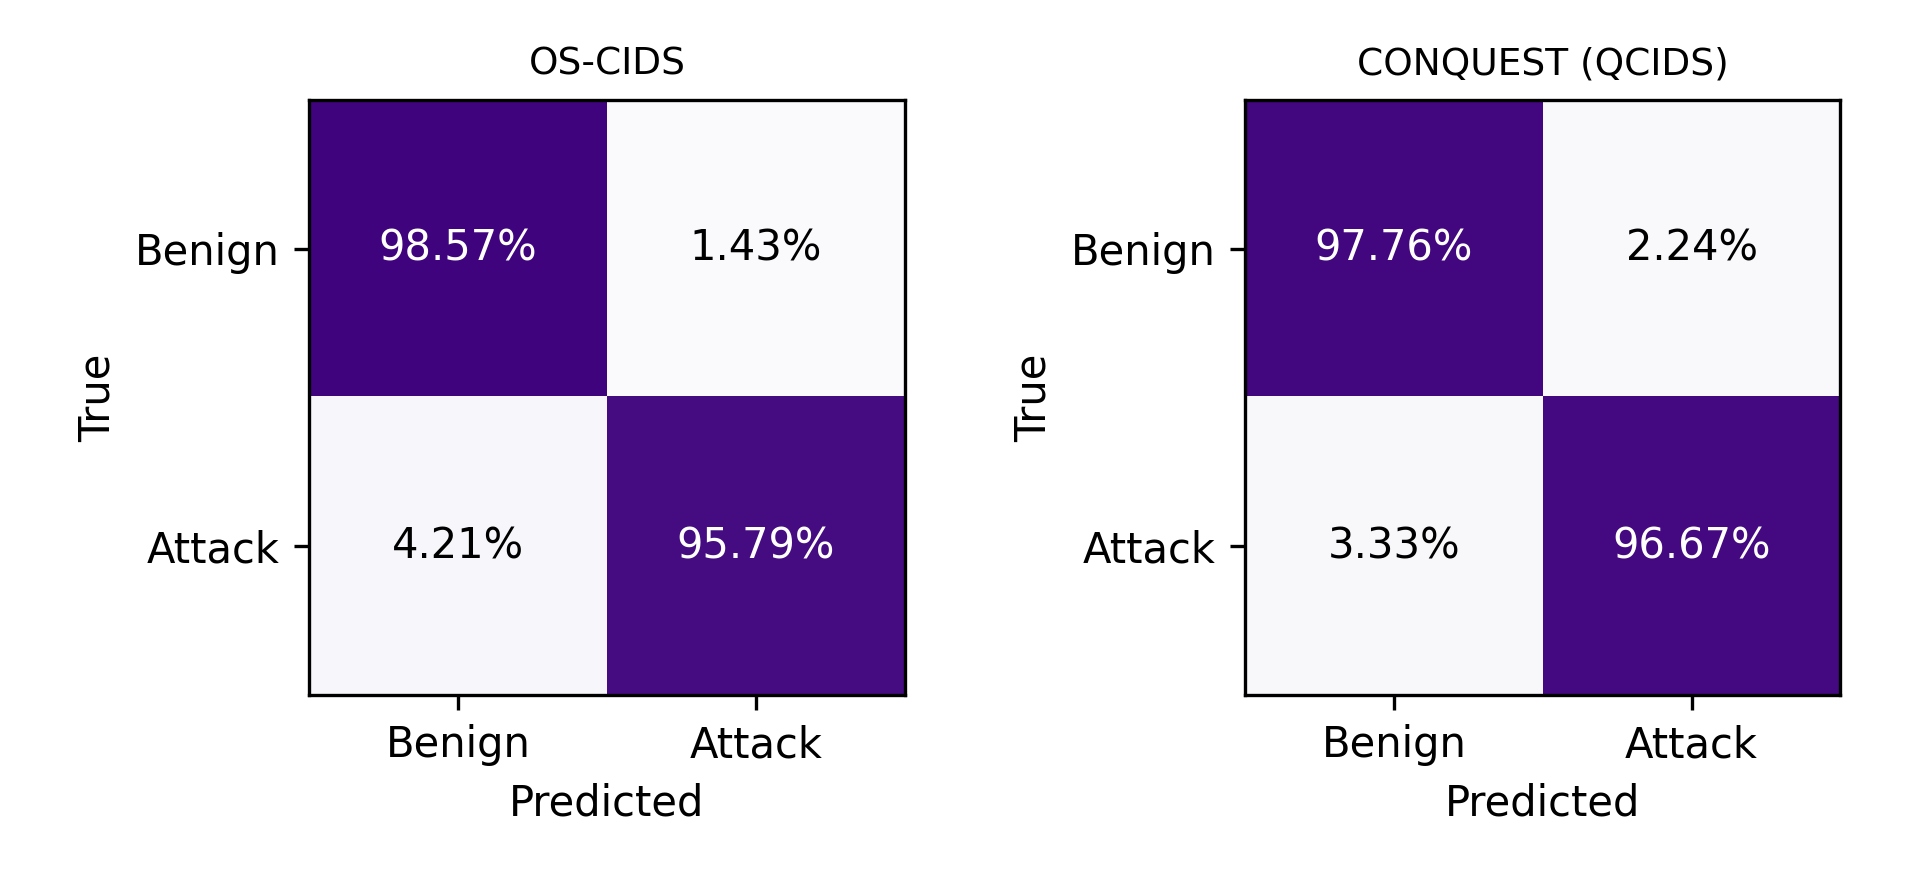
\includegraphics[width=\linewidth]{images/cm_conquest_vs_os.png}
    \caption{\textcolor{black}{Row-normalized confusion matrices of
    OS-CIDS and CONQUEST on the test set, averaged over ten seeds.}}
    
\end{figure}

\setcounter{figure}{4}
\begin{figure}[H]
    \centering
    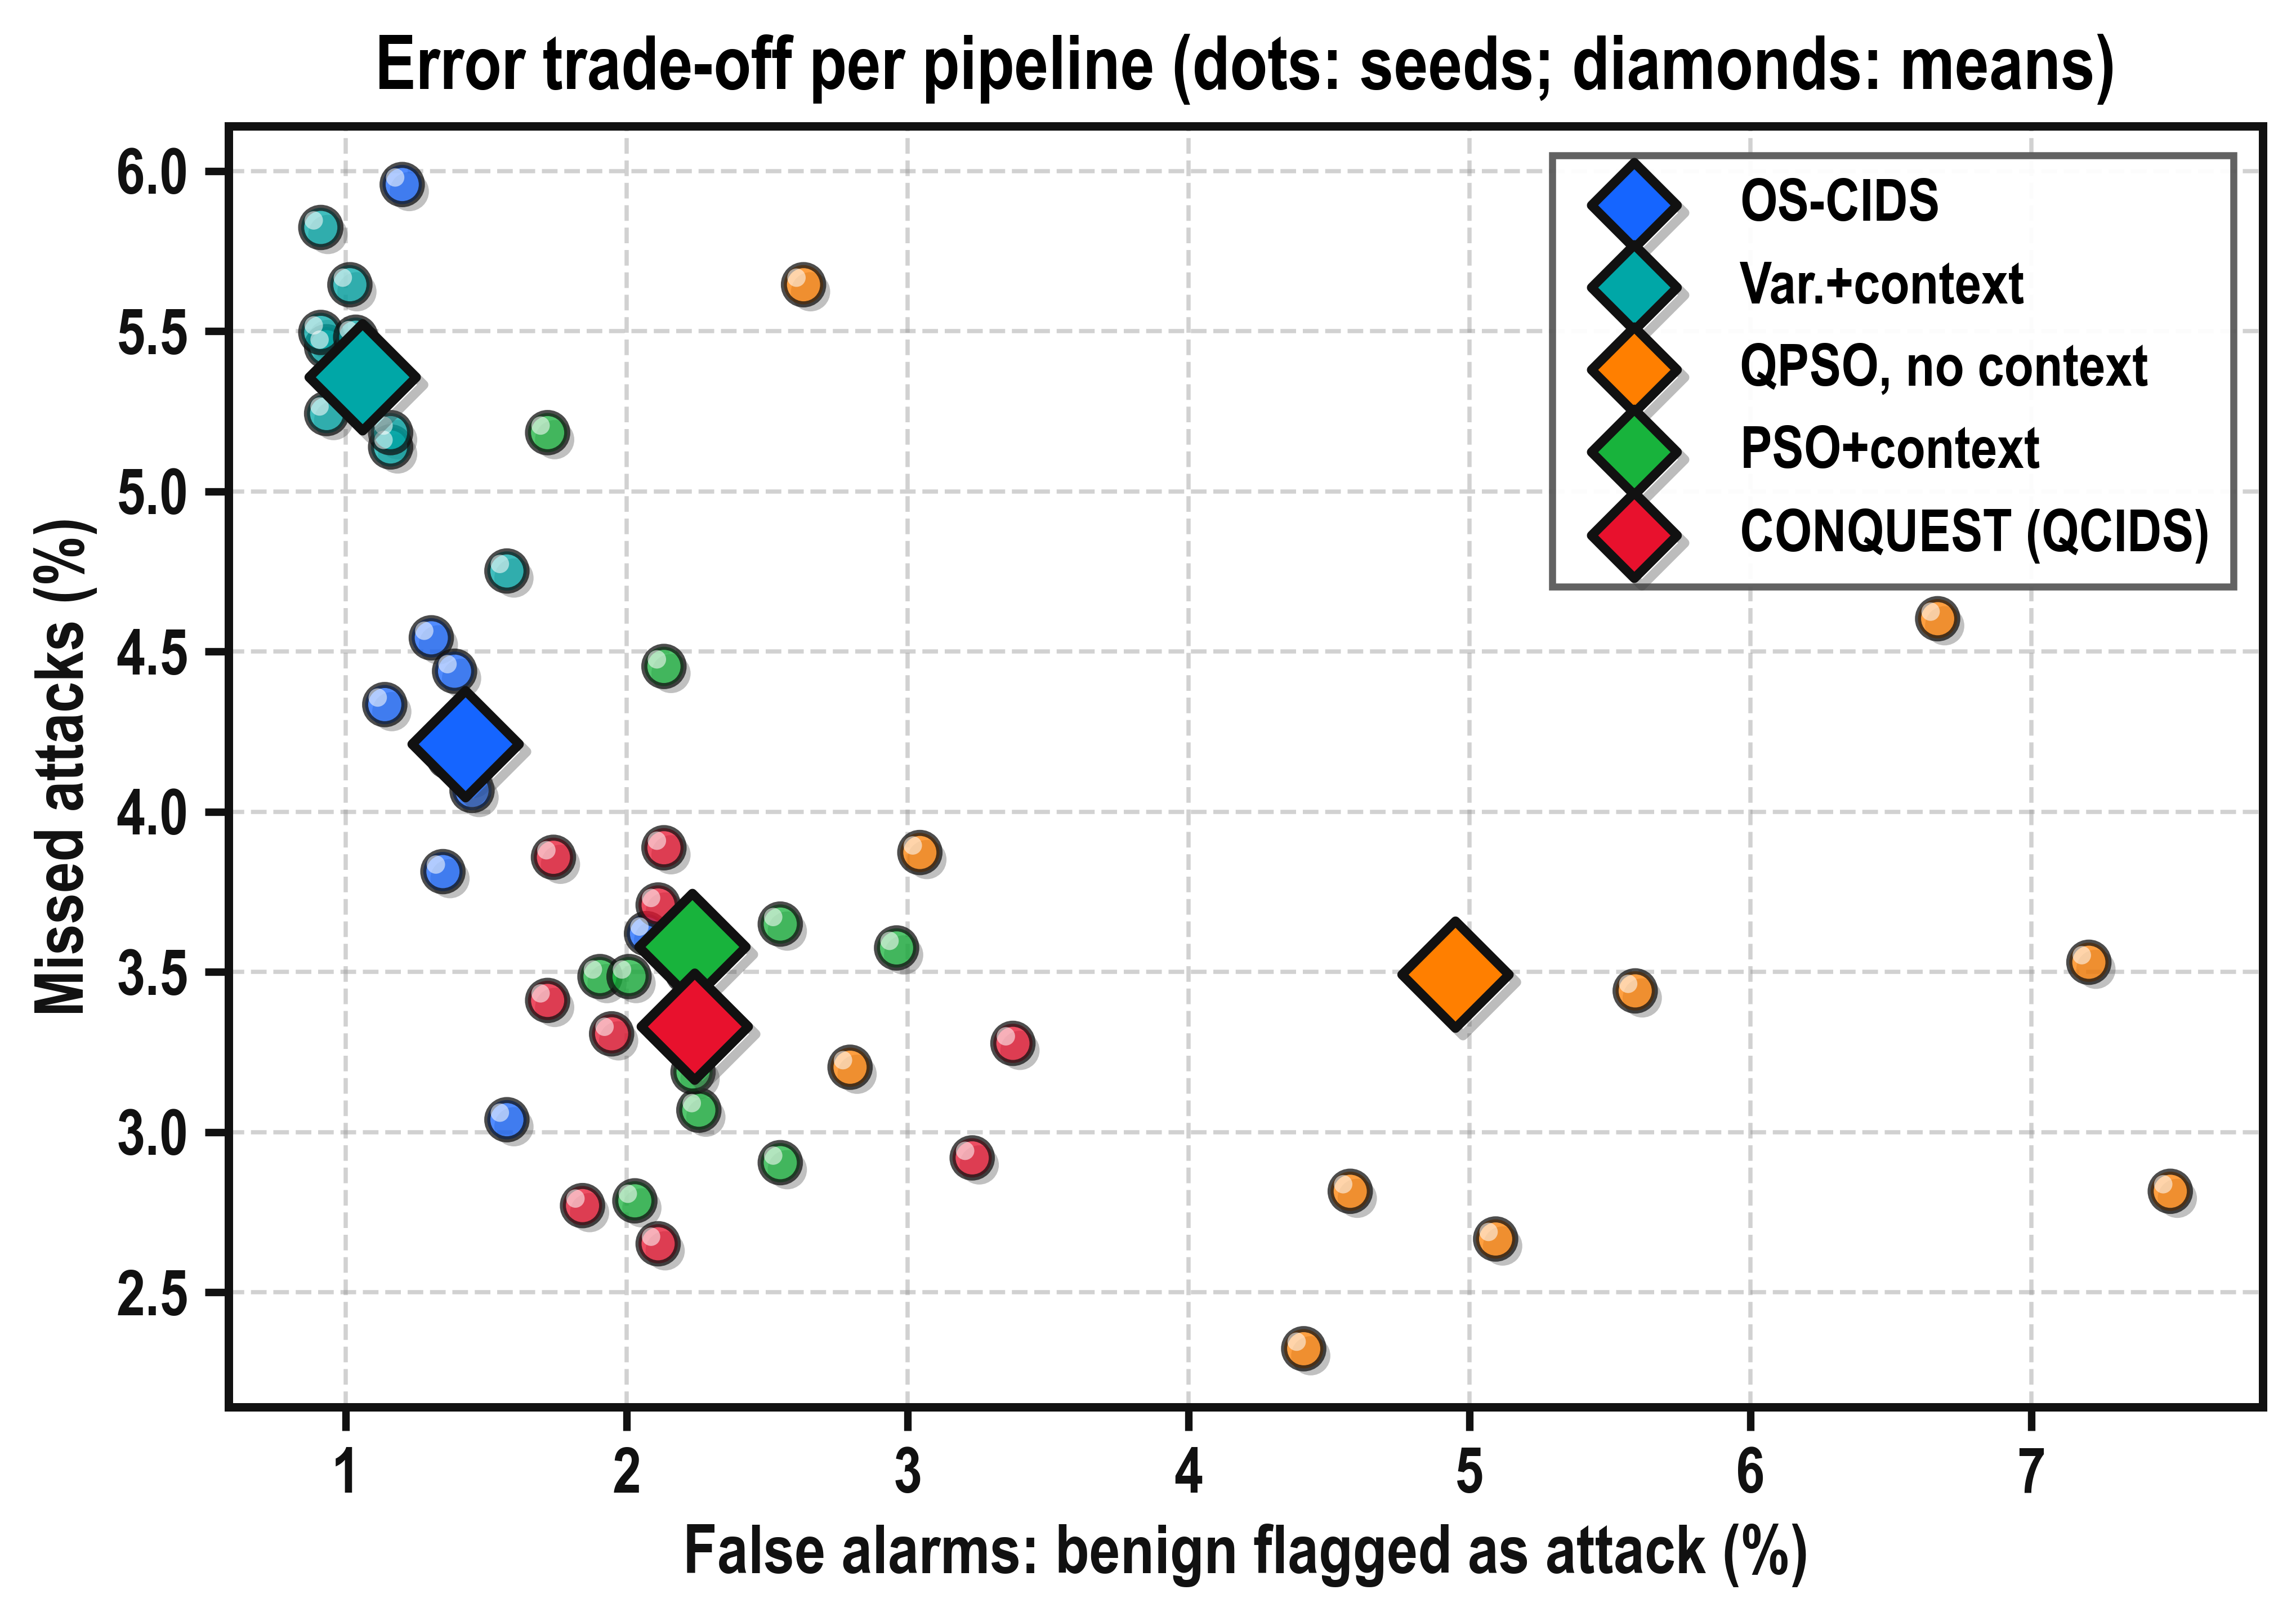
\includegraphics[width=\linewidth]{images/tradeoff_far_md.png}
    \caption{\textcolor{black}{False-alarm rate versus
    missed-attack rate of the five centralized pipelines. Dots:
    individual seeds; diamonds: means.}}
    
\end{figure}

\textcolor{black}{\textbf{Context features versus QPSO.} The
factorial ablation in Table~X separates
the two components, and neither helps on its own. Adding context
features to variance ranking lowers F1 by 0.51\,pp ($p=0.014$),
because variance ranking ignores labels and fills 14 of its 40 slots
with high-variance context counts, displacing informative
packet-length features. Replacing variance ranking by QPSO on static
features alone lowers F1 by 1.07\,pp ($p=0.002$), mainly through more
false alarms. Combined, however, context features and QPSO raise F1
by 1.23\,pp over QPSO alone and by 0.68\,pp over variance ranking with
context (both $p\le0.004$), and their interaction, $+1.74$\,pp
($p=0.002$), is the dominant effect. The gain of CONQUEST therefore
comes from combining context-aware representation with label-aware
selection, which keeps eight context features alongside complementary
static features, as listed in Table~XI.}

\setcounter{table}{9}
\begin{table}[H]
\centering
\scriptsize
\caption{\textcolor{black}{Factorial ablation of context features and QPSO over ten seeds.}}

\color{black}
\setlength{\tabcolsep}{3pt}
\begin{adjustbox}{max width=\linewidth}
\begin{tabular}{lccc}
\hline\toprule
\makecell[l]{F1 / FAR / MD\\(\%)} & \makecell{Variance\\ranking} & \makecell{QPSO\\($Q^{*}{=}6$)} & \makecell{Effect of\\QPSO (pp)} \\
\hline\toprule
Static only & 96.96 / 1.43 / 4.21 & 95.90 / 4.95 / 3.49 & \makecell{$-1.07$\\($p{=}0.002$)} \\
\makecell[l]{Static +\\context} & 96.45 / 1.06 / 5.36 & \textbf{97.13} / 2.24 / \textbf{3.33} & \makecell{$+0.68$\\($p{=}0.002$)} \\
\midrule
\makecell[l]{Effect of\\context (pp)} & \makecell{$-0.51$\\($p{=}0.014$)} & \makecell{$+1.23$\\($p{=}0.004$)} & \makecell{Interaction\\$+1.74$\\($p{=}0.002$)} \\
\hline\toprule
\end{tabular}
\end{adjustbox}
\end{table}

\setcounter{table}{10}
\begin{table}[H]
\centering
\scriptsize
\caption{\textcolor{black}{Deployed consensus mask at Q = 6; context features in italics.}}

\color{black}
\setlength{\tabcolsep}{2.5pt}
\renewcommand{\arraystretch}{1.02}
\begin{adjustbox}{max width=\linewidth}
\begin{tabular}{>{\raggedright\arraybackslash}p{3.0cm}c >{\raggedright\arraybackslash}p{3.0cm}c}
\hline\toprule
Feature & Freq. & Feature & Freq. \\
\hline\toprule
\textit{syn\_frac\_src\_60} & 1.0 & Fwd URG Flags & 0.6 \\
Fwd Packets/\allowbreak s & 0.9 & Packet Length Std & 0.6 \\
\textit{bytes\_rate\_src\_60} & 0.9 & SYN Flag Count & 0.6 \\
Fwd Packet Length Min & 0.8 & RST Flag Count & 0.6 \\
Fwd Header Length & 0.8 & PSH Flag Count & 0.6 \\
Average Packet Size & 0.8 & ACK Flag Count & 0.6 \\
Protocol & 0.7 & URG Flag Count & 0.6 \\
Fwd Packet Length Std & 0.7 & Fwd Segment Size Avg & 0.6 \\
Bwd Packet Length Min & 0.7 & Bwd Packet/\allowbreak Bulk Avg & 0.6 \\
Flow IAT Max & 0.7 & Bwd Bulk Rate Avg & 0.6 \\
Bwd IAT Max & 0.7 & Subflow Bwd Bytes & 0.6 \\
Bwd IAT Min & 0.7 & \textit{n\_flows\_src\_10} & 0.6 \\
Bwd Segment Size Avg & 0.7 & \textit{pkt\_rate\_src\_10} & 0.6 \\
\textit{n\_flows\_src\_60} & 0.7 & \textit{bytes\_rate\_src\_10} & 0.6 \\
\textit{n\_distinct\_dport\_10} & 0.7 & \textit{n\_proto\_switch\_60} & 0.6 \\
Total Length of Fwd Packet & 0.6 & Total Length of Bwd Packet & 0.5 \\
Bwd Packet Length Max & 0.6 & Fwd IAT Mean & 0.5 \\
Flow Packets/\allowbreak s & 0.6 & CWR Flag Count & 0.5 \\
Flow IAT Std & 0.6 & ECE Flag Count & 0.5 \\
Fwd IAT Std & 0.6 & Active Max & 0.5 \\
\hline\toprule
\end{tabular}
\end{adjustbox}
\end{table}

\textcolor{black}{\textbf{Quantum-inspired versus classical
search.} At an equal budget of 620 fitness evaluations, classical
binary PSO reaches a higher trace-ratio fitness than QPSO, 4919
versus 4401, in less time, 76\,s versus 106\,s, while the resulting
detectors are statistically indistinguishable ($p=0.23$ for F1 and
$p=0.49$ for MD). No quantum advantage is therefore claimed. In
CONQUEST, QPSO is one interchangeable instance of label-aware swarm
selection; its practical merits are a single interpretable control
parameter and robustness to that parameter, not superior accuracy.}

\textcolor{black}{\textbf{Choice of selector.} When
missed attacks are the costlier error, as for self-propagating worms,
label-aware selection with context features is preferable. When false
alarms dominate the operational cost, or labelled data are scarce,
variance ranking on static features gives a comparable F1 with the
fewest false alarms among the competitive pipelines, at negligible
cost and without labels. Context features should not be added to a
label-agnostic selector, and with a very tight feature budget,
variance ranking is again preferable, as shown next.}

\textcolor{black}{\textbf{Tight feature budgets.}
Table~XII repeats the selector comparison for $k=40$, 20,
and 10. With $k=40$, QPSO and PSO are equivalent, and QPSO exceeds
variance ranking on all five seeds. With $k=20$, QPSO has the highest
F1, 96.53\%, and the fewest missed attacks, 4.02\% against 4.67\% for
PSO and 5.98\% for variance ranking. With $k=10$, the ordering
reverses: variance ranking reaches 95.94\% F1 and beats QPSO, at
94.00\%, on all five seeds, while PSO reaches 94.34\%. The trace-ratio
fitness rewards low within-class variance, so with few slots the
swarm keeps only 1.6 of the 17 context features on average, whereas
variance ranking keeps five. Label-aware swarm selection therefore
pays off only when the budget leaves room for both context and static
features.}

\setcounter{table}{11}
\begin{table}[H]
\centering
\scriptsize
\caption{\textcolor{black}{Selector comparison under feature budgets of 40, 20, and 10 over five seeds; the consensus mask uses ten. Ctx.: context features kept. Wins: seeds on which QPSO has the higher F1.}}

\color{black}
\setlength{\tabcolsep}{3pt}
\begin{adjustbox}{max width=\linewidth}
\begin{tabular}{clccccc}
\hline\toprule
$k$ & Selector & F1 (\%) & FAR (\%) & MD (\%) & Ctx. & Wins \\
\hline\toprule
\multirow{3}{*}{40} & QPSO & 97.25$\pm$0.22 & 1.95 & 3.35 & 8.2 & -- \\
 & PSO & \textbf{97.28$\pm$0.15} & 2.15 & 3.15 & 6.6 & 3/5 \\
 & Variance & 96.43$\pm$0.15 & 1.07 & 5.38 & 14.0 & 5/5 \\
\midrule
\multirow{3}{*}{20} & QPSO & \textbf{96.53$\pm$0.42} & 2.72 & 4.02 & 1.8 & -- \\
 & PSO & 96.14$\pm$0.87 & 2.75 & 4.67 & 3.2 & 3/5 \\
 & Variance & 96.05$\pm$0.16 & 1.17 & 5.98 & 10.0 & 4/5 \\
\midrule
\multirow{3}{*}{10} & QPSO & 94.00$\pm$0.64 & 3.42 & 7.91 & 1.6 & -- \\
 & PSO & 94.34$\pm$0.51 & 3.73 & 7.08 & 1.4 & 0/5 \\
 & Variance & \textbf{95.94$\pm$0.30} & 1.15 & 6.18 & 5.0 & 0/5 \\
\midrule
40 & Consensus & 97.27$\pm$0.23 & 2.46 & 2.93 & 8.0 & -- \\
\hline\toprule
\end{tabular}
\end{adjustbox}
\end{table}

\textcolor{red}{Table~XIII
and Fig.~6 report the ablation over $Q=1$ to 8 with
ten seeds, re-executing QPSO in every run. Test F1 ranges only from
96.95\% at $Q=4$ to 97.20\% at $Q=1$; this 0.25\,pp spread of the
means is smaller than the average seed-to-seed standard deviation of
0.32\,pp. A Friedman test finds no significant effect of $Q$ on test
F1 ($\chi^2_7=6.07$, $p=0.53$), test AUC ($p=0.63$), or validation F1
($p=0.54$). The pre-declared validation rule selects $Q^{*}=6$, but
$Q^{*}=6$ is statistically indistinguishable from every other setting
(Holm-adjusted Wilcoxon $p\ge0.59$). It is therefore a reproducible
default selected on validation data, not a stability optimum. The two
settings beyond $Q=8$, evaluated with five seeds each, fall in the same band,
with test F1 of 97.30\% at $Q=9$ and 97.25\% at $Q=10$.}
\end{excerpt}
\begin{excerpt}
\setcounter{table}{12}
\begin{table}[H]
\centering
\caption{\textcolor{red}{Detection versus QPSO register size over ten seeds; last column: Holm-adjusted p-value against Q = 6.}}

\color{red}
\setlength{\tabcolsep}{3.5pt}
\resizebox{\textwidth}{!}{
\begin{adjustbox}{max width=\linewidth}
\begin{tabular}{ccccccccc}
\hline\toprule
$Q$ & Acc (\%) & F1 (\%) & AUC & MSE & FAR (\%) & MD (\%) & Val.\ F1 (\%) & $p$ vs.\ $Q{=}6$ \\
\hline\toprule
1 & 97.20$\pm$0.23 & 97.20$\pm$0.22 & 0.9926$\pm$0.0009 & 0.0243$\pm$0.0024 & 1.90$\pm$0.29 & 3.45$\pm$0.53 & 95.27$\pm$0.74 & 1.00 \\
2 & 97.08$\pm$0.17 & 97.09$\pm$0.17 & 0.9918$\pm$0.0011 & 0.0253$\pm$0.0019 & 2.19$\pm$0.58 & 3.44$\pm$0.55 & 95.00$\pm$1.58 & 1.00 \\
3 & 96.96$\pm$0.37 & 96.96$\pm$0.37 & 0.9916$\pm$0.0016 & 0.0263$\pm$0.0026 & 2.10$\pm$0.52 & 3.72$\pm$0.85 & 95.56$\pm$1.18 & 0.59 \\
4 & 96.94$\pm$0.49 & 96.95$\pm$0.49 & 0.9917$\pm$0.0021 & 0.0268$\pm$0.0039 & 1.93$\pm$0.29 & 3.87$\pm$0.81 & 95.38$\pm$1.58 & 1.00 \\
5 & 97.05$\pm$0.42 & 97.06$\pm$0.41 & 0.9925$\pm$0.0012 & 0.0249$\pm$0.0026 & 1.92$\pm$0.34 & 3.69$\pm$0.86 & 95.70$\pm$1.24 & 1.00 \\
\textbf{6}$^{*}$ & \textbf{97.13$\pm$0.31} & \textbf{97.13$\pm$0.31} & \textbf{0.9924$\pm$0.0016} & \textbf{0.0246$\pm$0.0028} & \textbf{2.24$\pm$0.58} & \textbf{3.33$\pm$0.44} & \textbf{96.00$\pm$1.04} & -- \\
7 & 97.17$\pm$0.32 & 97.17$\pm$0.32 & 0.9919$\pm$0.0012 & 0.0248$\pm$0.0024 & 2.05$\pm$0.33 & 3.39$\pm$0.69 & 95.75$\pm$0.84 & 1.00 \\
8 & 97.07$\pm$0.26 & 97.08$\pm$0.26 & 0.9918$\pm$0.0008 & 0.0249$\pm$0.0013 & 2.03$\pm$0.34 & 3.57$\pm$0.52 & 95.59$\pm$0.95 & 1.00 \\
\hline\toprule
\end{tabular}
\end{adjustbox}}
\end{table}

\textcolor{red}{Together with Fig.~3,
these results give a consistent picture. $Q$ strongly changes how the
swarm searches, but with 40 of 86 features, including 17 informative
context features, many subsets support equally accurate detectors,
so the classifier is robust to $Q$. In practice, $Q$ needs no fine
tuning: every setting from 1 to 8 yields between 96.95\% and 97.20\%
test F1 over ten seeds, and $Q=9$ and 10 fall in the same band.}
\end{excerpt}
\setcounter{figure}{5}
\begin{figure}[H]
\centering
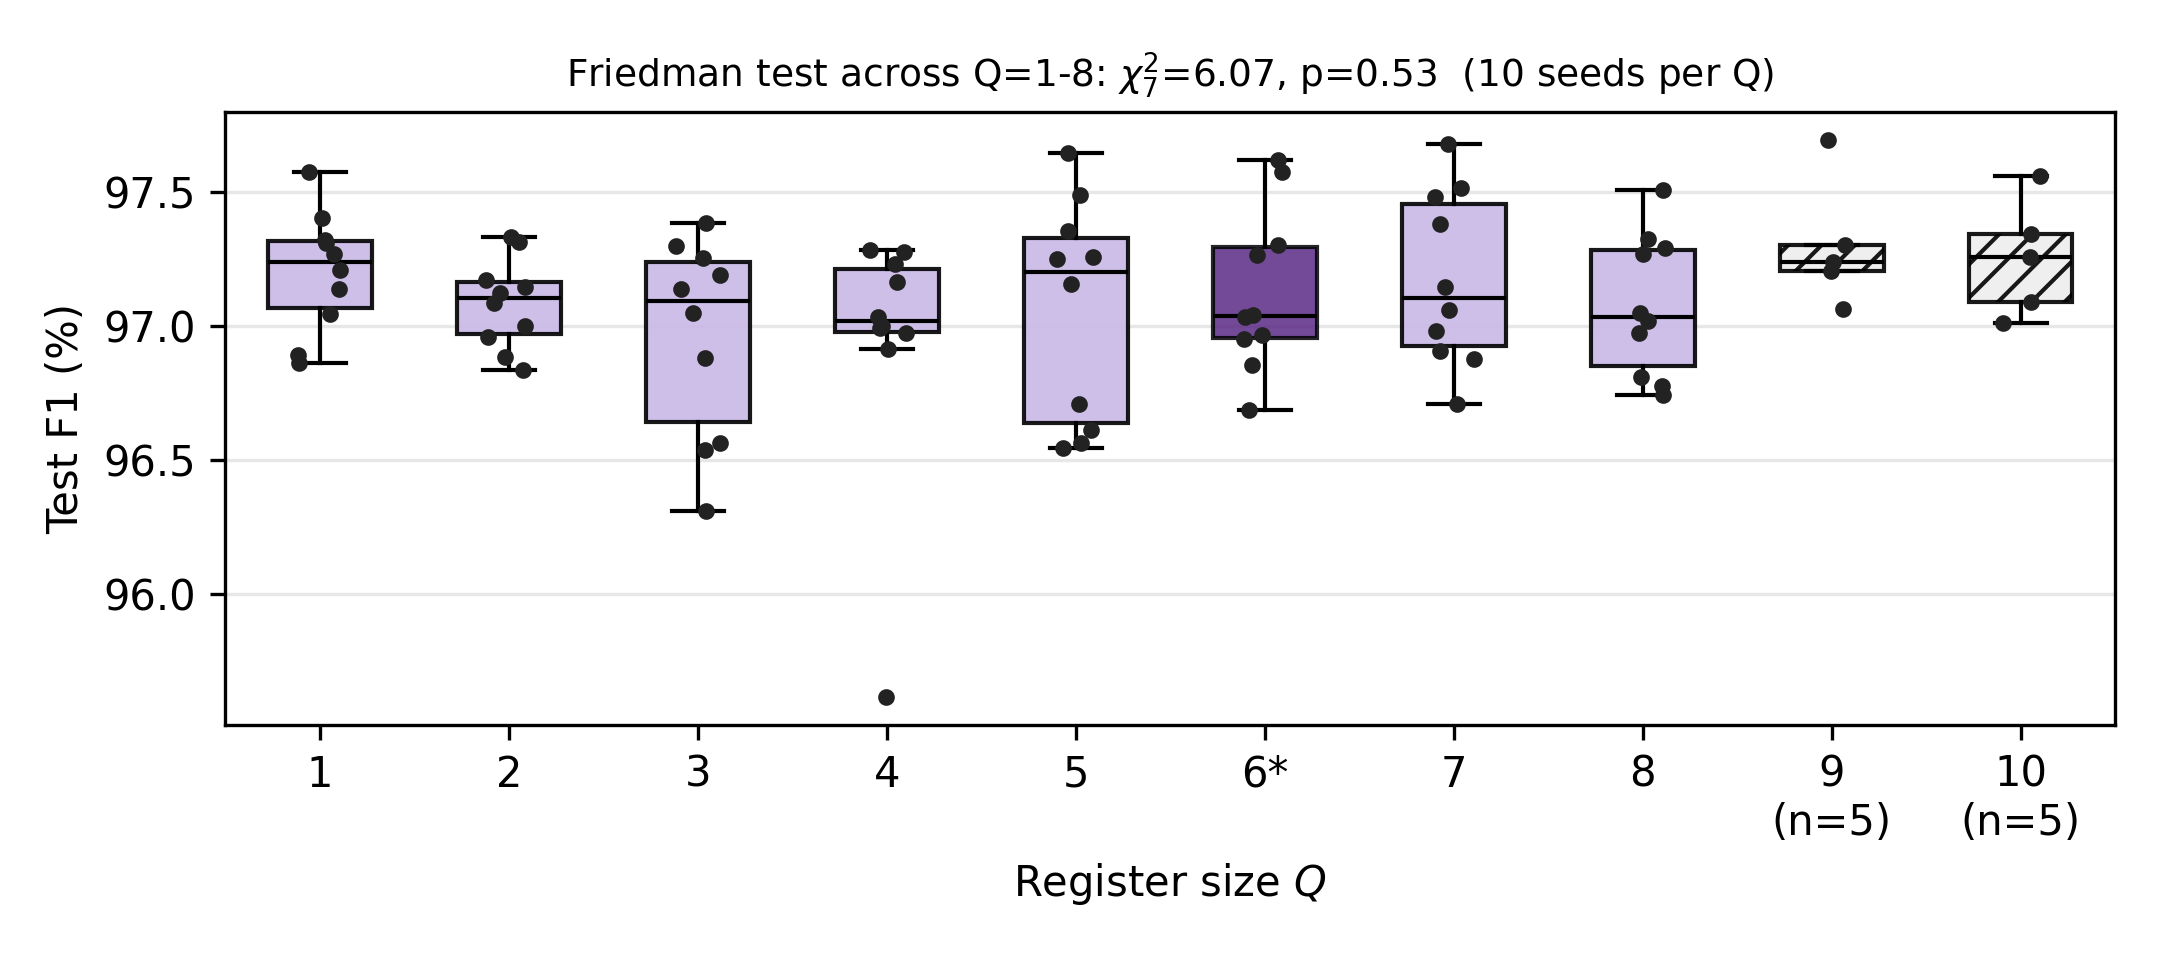
\includegraphics[width=\linewidth]{images/q_ablation_boxplot.png}
\caption{\textcolor{red}{Test F1 versus QPSO register size; hatched boxes use five seeds, the others ten.}}

\end{figure}

%% ---------------------------------------------------------------------
\review{1.3}{In Section III-B and Table III, manuscript pp.~5--7, the QPSO search uses 20 particles and 30 iterations, but no sensitivity analysis shows that this budget is sufficient. The degradation at $Q=7$--8 may reflect insufficient search rather than excessive qubit expressiveness. The authors should test whether larger particle or iteration budgets change the apparent optimum.}

\reply We thank the reviewer for this insightful comment and have added the
requested sensitivity analysis. The search alone was repeated for $Q=1$ to 10
with up to eight times the default number of fitness evaluations, and full
detectors were trained for $Q=6$ to 10 with 20 or 40 particles and 30 or 60
iterations, and for all $Q$ from 1 to 10 at the largest budget, with five
seeds each. A larger budget raises the best fitness found (Friedman
$p<10^{-4}$), but it does not improve detection: test F1 stays within
96.9--97.3\% in every cell, with no budget effect (Friedman $p=0.50$), and
validation F1 even decreases slightly at the largest budget. No degradation
at $Q=7$ or 8 appears at any budget, and the validation-selected $Q$ changes
with the budget, as expected when no setting is genuinely better. The
degradation reported in the previous version came from three seeds with a
single QPSO run per $Q$ and is not reproduced with ten seeds. The default
budget of 20 particles and 30 iterations is therefore sufficient for
detection and is retained at the lowest cost.

\loc{(a) Pages 7--8: Added the design of the search-budget experiments to Section III-B}
\begin{excerpt}
\mshead{III-B}{Variable-Qubit QPSO Feature Selection}


QPSO learns a sparse binary feature mask
$\mathbf{m}\in\{0,1\}^d$ that gates the normalized input:
\begin{equation}
\tilde{\mathbf{z}} = \mathbf{m}\odot\mathbf{z}_n,\quad
\|\mathbf{m}\|_0 = k \ll d,
\tag{6}
\end{equation}
where $\odot$ denotes element-wise multiplication.
\textcolor{black}{Each of the $P$ particles $i$ holds a
non-negative amplitude vector $\mathbf{a}_i\in\mathbb{R}_{\ge 0}^{d}$
with $\sum_j a_{i,j}=1$, one amplitude per feature, so the particle
dimension is $d$ for every $Q$. The register size $Q$ enters the
search at three points. First, amplitudes are initialized at the
uniform amplitude of a $Q$-qubit register plus Gaussian noise; after
normalization, only the relative perturbation
$\rho(Q)=2^{Q/2}/(Q^{2}+1)$ matters:}
\begin{equation}
\textcolor{black}{a_{i,j}^{(0)} \propto \Bigl|\,2^{-Q/2} +
\tfrac{\xi_{i,j}}{Q^{2}+1}\Bigr|,\quad
\xi_{i,j}\sim\mathcal{N}(0,1).}
\tag{7}
\end{equation}
\textcolor{black}{Second, at iteration $t$, each particle is
rotated toward its personal-best amplitude $\mathbf{a}_i^{\rm pb}$
and the global-best amplitude $\mathbf{a}^{\rm gb}$ by an angle whose
upper bound decreases with $Q$:}
\begin{align}
\textcolor{black}{\phi_t} &\textcolor{black}{= \frac{\pi}{2Q}\Bigl(1-\frac{t}{I}\Bigr),}
\tag{8}\\
\textcolor{black}{\mathbf{a}_i} &\textcolor{black}{\leftarrow \mathbf{a}_i
+ r_1\cos\phi_t\,(\mathbf{a}_i^{\rm pb}-\mathbf{a}_i)
+ r_2\sin\phi_t\,(\mathbf{a}^{\rm gb}-\mathbf{a}_i),}
\tag{9}
\end{align}
\textcolor{black}{with $r_1,r_2\sim\mathcal{U}(0,1)$ drawn per
particle and iteration. Third, each amplitude independently
``collapses'' to a fresh random value with a probability that decays
exponentially in $Q$, and the vector is then renormalized:}
\begin{equation}
\textcolor{black}{a_{i,j} \leftarrow u_{i,j}\sim\mathcal{U}(0,1)
\ \text{w.p. } 2^{-Q},\quad
\mathbf{a}_i \leftarrow |\mathbf{a}_i| / \|\mathbf{a}_i\|_1 .}
\tag{10}
\end{equation}
\textcolor{black}{A mask is obtained by measurement: $k$
distinct feature indices are drawn without replacement with
probabilities $\pi_{i,j}=a_{i,j}^{2}/\sum_{l}a_{i,l}^{2}$, and
$m_{i,j}=1$ for the drawn indices,}
\begin{equation}
\textcolor{black}{\mathbf{m}_i = \textsc{Measure}_k(\boldsymbol{\pi}_i),
\qquad \|\mathbf{m}_i\|_0 = k .}
\tag{11}
\end{equation}
\textcolor{black}{Each run returns $\mathbf{m}^{*}$, the
highest-fitness mask measured during the search, as in standard PSO.
Hence $k$ is a fixed design parameter, set to 40 in all experiments,
and $Q$ shapes \emph{which} $k$ features are found, not how many.
Algorithm~1 summarizes the procedure, and
Table~V lists the constants set by each $Q$.}
\textcolor{black}{Because a single run's mask depends on its
seed, the deployed detector uses a consensus mask
$\mathbf{m}^{*}_{\rm cons}$: the $k$ features selected most often
across the ten QPSO runs at the selected $Q^{*}$, with ties broken by
the summed fitness of the runs that selected them. All ten runs use
$\mathcal{D}_{\rm tr}$ only, so the consensus uses no validation or
test data.}

\setcounter{table}{4}
\begin{table}[H]
\centering
\scriptsize
\caption{\textcolor{black}{Search constants set by the
register size for the 86 input features.}}

\setlength{\tabcolsep}{4pt}
\renewcommand{\arraystretch}{1.05}
\color{black}
\begin{adjustbox}{max width=\linewidth}
\begin{tabular}{cccccc}
\hline\toprule
$Q$ & \makecell{Initial\\perturb.} & \makecell{Max.\ rot.\\(deg)} & \makecell{Reset\\prob.} & \makecell{Resets per\\particle-iter.} & Regime \\
\hline\toprule
1  & 0.71 & 90.0 & 0.500  & 43.0 & near-random \\
2  & 0.40 & 45.0 & 0.250  & 21.5 & exploratory \\
3  & 0.28 & 30.0 & 0.125  & 10.8 & exploratory \\
4  & 0.24 & 22.5 & 0.063  & 5.38 & balanced \\
5  & 0.22 & 18.0 & 0.031  & 2.69 & balanced \\
6  & 0.22 & 15.0 & 0.016  & 1.34 & balanced \\
7  & 0.23 & 12.9 & 0.008  & 0.67 & exploitative \\
8  & 0.25 & 11.3 & 0.004  & 0.34 & exploitative \\
9  & 0.29 & 10.0 & 0.002  & 0.17 & near-frozen \\
10 & 0.32 & 9.0  & 0.001  & 0.08 & near-frozen \\
\hline\toprule
\end{tabular}
\end{adjustbox}
\end{table}

\setcounter{algorithm}{0}
\begin{algorithm}[H]
\caption{\textcolor{black}{Variable-qubit QPSO feature
selection. Steps commented with Q are the only ones that depend on
the register size.}}

\color{black}
\small
\begin{algorithmic}[1]
\Require $\mathbf{Z}_{\rm tr}\in[0,1]^{N\times d}$, labels $\mathbf{y}_{\rm tr}$, register size $Q$, particles $P$, iterations $I$, subset size $k$
\Ensure Mask $\mathbf{m}^{*}\in\{0,1\}^{d}$ with $\|\mathbf{m}^{*}\|_0=k$
\For{$i=1$ to $P$}
  \State $\mathbf{a}_i\gets$ Eq.~(7), normalized \Comment{$Q$}
  \State $\mathbf{m}_i\gets\textsc{Measure}_k(\mathbf{a}_i)$; $J_i\gets\mathcal{J}(\mathbf{m}_i)$ on $\mathcal{D}_{\rm tr}$
  \State $\mathbf{a}_i^{\rm pb}\gets\mathbf{a}_i$; $J_i^{\rm pb}\gets J_i$
\EndFor
\State $i^{\star}\gets\arg\max_i J_i$; $\mathbf{a}^{\rm gb}\gets\mathbf{a}_{i^{\star}}$; $\mathbf{m}^{*}\gets\mathbf{m}_{i^{\star}}$; $J^{*}\gets J_{i^{\star}}$
\For{$t=0$ to $I-1$}
  \State $\phi_t\gets\frac{\pi}{2Q}(1-t/I)$ \Comment{$Q$}
  \For{$i=1$ to $P$}
    \State $\mathbf{a}_i\gets$ rotation toward $\mathbf{a}_i^{\rm pb},\mathbf{a}^{\rm gb}$, Eq.~(9)
    \State reset each $a_{i,j}$ w.p.\ $2^{-Q}$; normalize, Eq.~(10) \Comment{$Q$}
    \State $\mathbf{m}_i\gets\textsc{Measure}_k(\mathbf{a}_i)$, Eq.~(11); $J_i\gets\mathcal{J}(\mathbf{m}_i)$
    \If{$J_i>J_i^{\rm pb}$}
      \State $\mathbf{a}_i^{\rm pb}\gets\mathbf{a}_i$; $J_i^{\rm pb}\gets J_i$
    \EndIf
    \If{$J_i>J^{*}$}
      \State $\mathbf{a}^{\rm gb}\gets\mathbf{a}_i$; $\mathbf{m}^{*}\gets\mathbf{m}_i$; $J^{*}\gets J_i$
    \EndIf
  \EndFor
\EndFor
\State \Return $\mathbf{m}^{*}$ \Comment{$P(I+1)$ fitness evaluations}
\end{algorithmic}
\end{algorithm}

\textcolor{black}{Table~V shows
how $Q$ shapes the search. With a single qubit, the rotation bound is
$\pi/2$ and half of all amplitudes are reset at every iteration, so
the search is close to random sampling. As $Q$ grows, the bound
shrinks, the personal-best term dominates the update, and from $Q=7$
onward fewer than one amplitude per particle is reset at each
iteration. $Q$ therefore
moves the search from exploration to exploitation, with a risk of
premature convergence at large $Q$ under a finite budget. Beyond
$Q=8$, resets are rare and the pull toward the global best is weak,
so the search stays close to its initialization. The trained-detector
ablation therefore covers $Q=1$ to $8$, and the budget analysis
extends the range to $Q=10$ to confirm this behavior.}

\textcolor{black}{CONQUEST is quantum-\emph{inspired} and runs
on classical hardware: no $2^{Q}$-dimensional state vector is
simulated, and the particle dimension is $d$ for every $Q$. The term
``qubit'' refers to the register whose uniform amplitude $2^{-Q/2}$
and collapse probability $2^{-Q}$ motivate the three constants
above. $Q$ is thus a single interpretable hyperparameter that sets
the exploration schedule of the swarm, not a measure of model
capacity.}

\textcolor{black}{Fig.~3 confirms this
behavior empirically. Algorithm~1 is run on
$\mathcal{D}_{\rm tr}$ for $Q=1$ to $10$ with ten seeds, without
classifier training, and three regimes appear. At $Q=1$, the
amplitude entropy falls only to 0.75, because half of the amplitudes
are reset at every iteration, and the swarm keeps sampling almost
uniformly. For $Q=4$ to $7$, the entropy falls to 0.25--0.35 within a
few iterations and swarm diversity drops: the search concentrates on
a feature subset. For $Q\ge 9$, the entropy stays at 0.54--0.66,
because small rotations and rare resets barely move the particles.
The best fitness peaks at $Q=4$ and is lower at both extremes,
although the differences are within the seed-to-seed spread.
Returning the best evaluated mask matters most at large $Q$: a fresh
measurement of the final global-best amplitude retains 91\% of the
best fitness at $Q=1$ but only 44--52\% at $Q\ge9$, because those
amplitudes remain spread out and rarely reproduce the best subset.}

\setcounter{figure}{2}
\begin{figure}[H]
\centering

\includegraphics[width=0.95\linewidth]{images/qpso_dynamics_vs_Q.png}
\caption{\textcolor{black}{QPSO search dynamics versus register size over ten seeds: measurement entropy (left), mask diversity (middle), and best fitness (right).}}

\end{figure}

\textcolor{black}{Each measured mask is scored by the
Fisher trace ratio of its selected features, a class-separability
criterion referred to below as the trace-ratio fitness,}
\begin{equation}
\textcolor{black}{\mathcal{J}(\mathbf{m}) =
\frac{\sum_{c}n_c\,\|\boldsymbol{\mu}_c^{\mathbf{m}}-
\boldsymbol{\mu}^{\mathbf{m}}\|_2^{2}}
{\sum_{c}\sum_{j:m_j=1}\mathrm{Var}_c(z_j)+\epsilon},}
\tag{12}
\end{equation}
\textcolor{black}{where $c\in\{\text{benign},\text{attack}\}$, $n_c$
and $\boldsymbol{\mu}_c^{\mathbf{m}}$ are the class count and class
mean of the selected features, $\boldsymbol{\mu}^{\mathbf{m}}$ is
their overall mean, and $\epsilon=10^{-10}$. Personal and global
bests are updated when $\mathcal{J}$ improves. $\mathcal{J}$ is a
filter criterion that needs no classifier training, so one run with
20 particles and 30 iterations costs 620 fitness evaluations.}
\textcolor{red}{One run takes a median of 1.8\,min on the
host of Table~VI, and 5.0\,min at the largest
trained budget of 40 particles and 60 iterations.}

\setcounter{table}{5}
\begin{table}[H]
\centering
\caption{Experimental environment and implementation settings.}

\def\rc#1{\textcolor{red}{#1}}
\setlength{\tabcolsep}{8pt}
\renewcommand{\arraystretch}{1.3}
\begin{adjustbox}{max width=\linewidth}
\begin{tabular}{l l l l}
\hline\toprule
\textbf{Block} & \textbf{Item} & \textbf{Setting} & \textbf{Scope} \\
\hline\toprule
Environment & Platform & Windows 10, CPU only & All runs \\
 & Framework & TensorFlow 2.20.0, Python 3.13.5 & Training and inference \\
 & Determinism & \texttt{TF\_DETERMINISTIC\_OPS=1} & Seed-controlled \\
\midrule
Data & \rc{Subsample} & \rc{80k flows, class-balanced} & \rc{Fixed seed 42} \\
 & \rc{Split} & \rc{Blocked temporal, 70/15/15} & \rc{500-flow blocks} \\
 & Window length & $T=10$ flows & All regimes \\
 & \rc{Batch size} & \rc{32 centralized, 64 federated} & \rc{All regimes} \\
\midrule
Training & \rc{Optimizer} & \rc{SGD, Nesterov momentum 0.9} & \rc{Centralized and federated} \\
 & Learning rate & $10^{-3}$ & Centralized and federated \\
 & \rc{Stopping} & \rc{At most 35 epochs, patience 6} & \rc{Validation loss} \\
 & \rc{KL weight} & \rc{$\gamma=10^{-3}$} & \\
\midrule
Model & \rc{Encoder} & \rc{LSTM 256, 2-head attention, LSTM 128} & \rc{Dropout 0.2} \\
 & \rc{Latent size} & \rc{64} & \rc{LSTM(+VAE) variants} \\
\midrule
QPSO & Particles, iterations & $P=20$, $I=30$ & Default budget \\
 & \rc{Budget sensitivity} & \rc{$P=20$ or 40, $I=30$ or 60} & \rc{Five seeds} \\
 & \rc{Selected features} & \rc{$k=40$, fitness on $\mathcal{D}_{\rm tr}$} & \rc{All selectors} \\
 & \rc{Register size} & \rc{$Q=1$ to 8; $Q=9$, 10} & \rc{Ten seeds; five seeds} \\
\midrule
Federated & \rc{Clients} & \rc{$K=5$; 10 and 20 for sensitivity} & \rc{Full participation} \\
 & \rc{Rounds, local epochs} & \rc{$R=30$, $E=2$} & \rc{All FL experiments} \\
 & \rc{Mask construction} & \rc{Proxy (default), vote, central} & \rc{Shared by all clients} \\
 & Aggregators & FedAvg, SCAFFOLD, FLAME & Same partitions \\
\hline\toprule
\end{tabular}
\end{adjustbox}
\end{table}

\textcolor{black}{Table~VII lists the data
used by every step that fits, selects, or stops. The
QPSO fitness in Eq.~(12) is a label-based filter criterion
evaluated on $\mathcal{D}_{\rm tr}$ only; it contains no F1, AUC,
MSE, or error-balance terms and therefore has no weights to tune.
$Q^{*}$ is chosen on $\mathcal{D}_{\rm va}$, and early stopping and
the learning-rate schedule monitor the $\mathcal{D}_{\rm va}$ loss.
The search budget, $k=40$, and the classifier hyperparameters were
fixed before the experiments. $\mathcal{D}_{\rm te}$ is evaluated
once per trained model, after training, to report the final
metrics. In federated training, the global F1 on $\mathcal{D}_{\rm te}$
is also logged after every round to measure convergence, but it never
selects a round, a model, or a setting.}

\setcounter{table}{6}
\begin{table}[H]
\centering
\scriptsize
\caption{\textcolor{black}{Data used by each fitting,
selection, and stopping step. The test set is used only for
reporting.}}

\color{black}
\setlength{\tabcolsep}{3pt}
\renewcommand{\arraystretch}{1.05}
\begin{adjustbox}{max width=\linewidth}
\begin{tabular}{p{2.6cm} p{3.6cm} c}
\hline\toprule
\textbf{Step} & \textbf{Data used} & \textbf{Test set?} \\
\hline\toprule
Zero-variance filter & $\mathcal{D}_{\rm tr}$ (features only) & no \\
Context features & Earlier flows of the same source, unlabelled & no \\
Min--max normalization & $\mathcal{D}_{\rm tr}$ (features only) & no \\
QPSO / PSO fitness & $\mathcal{D}_{\rm tr}$ & no \\
Variance selection (OS-CIDS) & $\mathcal{D}_{\rm tr}$ (features only) & no \\
Consensus mask & Ten masks fitted on $\mathcal{D}_{\rm tr}$ & no \\
Selection of $Q^{*}$ & $\mathcal{D}_{\rm va}$, mean F1 over seeds & no \\
Early stopping, LR schedule & $\mathcal{D}_{\rm va}$ loss & no \\
Budget, $k$, hyperparameters & Fixed a priori & no \\
Decision rule & Fixed $\arg\max$ & no \\
FL masks (proxy/vote/central) & Proxy slice / client partitions / all of $\mathcal{D}_{\rm tr}$ & no \\
FL stopping & Fixed $R=30$ rounds & no \\
\midrule
Reported metrics & $\mathcal{D}_{\rm te}$, once per trained model & yes \\
FL per-client metrics & Client-matched windows of $\mathcal{D}_{\rm te}$, final model only & yes \\
FL convergence ($R_{99}$) & Per-round global F1 on $\mathcal{D}_{\rm te}$, reporting only & yes \\
\hline\toprule
\end{tabular}
\end{adjustbox}
\end{table}

\textcolor{black}{The register size $Q^{*}$ is the value in
$Q=1$ to $8$ with the highest mean validation F1 over ten seeds, with
ties going to the smaller $Q$; this rule selects $Q^{*}=6$. As Section~IV-A
shows, $Q$ has no significant effect on test F1 within this range, so $Q^{*}$ is a
reproducible default rather than an optimum.}

\textcolor{red}{Two experiments test whether the default
budget of 20 particles and 30 iterations is sufficient and whether
the conclusions about $Q$ depend on it. First, the search alone is
repeated for $Q=1$ to $10$ with 40 particles and 60 iterations, and
with 80 particles and 60 iterations. Second, full detectors are
trained for $Q=6$ to $10$ with 20 or 40 particles and 30 or 60
iterations, and for $Q=1$ to $10$ with 40 particles and 60
iterations, using five seeds each. Budget effects are tested with
Friedman and Wilcoxon signed-rank tests, blocked by register size
and seed.}
\end{excerpt}

\loc{(b) Pages 13--15: Added the search-budget sensitivity study to Section IV-A}
\begin{excerpt}
\mshead{IV-A}{Centralized Cyberworm Detection Performance}


Table~IX reports centralized detection
performance \textcolor{black}{of five pipelines that share the
classifier, the data protocol, and $k=40$. They differ only in the
feature representation, static only or static plus context, and in
the selector: variance ranking, classical PSO, or QPSO. They are named
OS-CIDS (variance ranking, static only), Var.+context (variance
ranking, static plus context), QPSO, no context, PSO+context
(classical PSO, static plus context), and CONQUEST (QPSO, static plus
context). All metrics
are computed on $\mathcal{D}_{\rm te}$, which contains 41.8\% benign
and 58.2\% attack windows, and averaged over ten seeds; accuracy and
weighted F1 nearly coincide because both classes are well
represented.}

\setcounter{table}{8}
\begin{table}[H]
\centering
\caption{\textcolor{black}{Centralized detection over ten seeds, with Wilcoxon p-values against CONQUEST. \textsuperscript{\textdagger}Conference result~{[9]}, not directly comparable.}}

\color{black}
\setlength{\tabcolsep}{3pt}
\resizebox{\textwidth}{!}{
\begin{adjustbox}{max width=\linewidth}
\begin{tabular}{lccccccccc}
\hline\toprule
\textbf{Pipeline} & Acc (\%) & F1 (\%) & AUC & MSE & FAR (\%) & MD (\%) & $p$ (F1) & $p$ (MD) & Selection (s) \\
\hline\toprule
S-CIDS~{[9]}\textsuperscript{\textdagger} & 85.14 & 80.62 & -- & -- & -- & -- & -- & -- & -- \\
\midrule
OS-CIDS & 96.95$\pm$0.39 & 96.96$\pm$0.39 & 0.9944$\pm$0.0011 & 0.0245$\pm$0.0025 & 1.43$\pm$0.26 & 4.21$\pm$0.76 & 0.322 & 0.004 & 0.0 \\
Var.+context & 96.44$\pm$0.11 & 96.45$\pm$0.11 & 0.9925$\pm$0.0007 & 0.0291$\pm$0.0015 & 1.06$\pm$0.20 & 5.36$\pm$0.30 & 0.002 & 0.002 & 0.1 \\
QPSO, no context & 95.90$\pm$0.83 & 95.90$\pm$0.83 & 0.9879$\pm$0.0030 & 0.0329$\pm$0.0060 & 4.95$\pm$1.80 & 3.49$\pm$1.00 & 0.004 & 0.824 & 68.0 \\
PSO+context & 96.98$\pm$0.40 & 96.99$\pm$0.39 & 0.9918$\pm$0.0018 & 0.0254$\pm$0.0031 & 2.23$\pm$0.37 & 3.58$\pm$0.73 & 0.232 & 0.492 & 75.6 \\
\textbf{CONQUEST (QCIDS)} & \textbf{97.13$\pm$0.31} & \textbf{97.13$\pm$0.31} & \textbf{0.9924$\pm$0.0016} & \textbf{0.0246$\pm$0.0028} & \textbf{2.24$\pm$0.58} & \textbf{3.33$\pm$0.44} & -- & -- & 105.9 \\
\hline\toprule
\end{tabular}
\end{adjustbox}}
\end{table}

\textbf{S-CIDS}, the conference baseline~{[9]},
achieves 85.14\% accuracy and 80.62\% F1. \textcolor{black}{This single-run result was
obtained with a random split of pooled data and is quoted for
reference only; it is not comparable with the leakage-free results
below.}

\textcolor{black}{\textbf{Overall comparison.}
CONQUEST reaches the highest mean F1, $97.13\pm0.31\%$, and the lowest
missed-attack rate, 3.33\%. Its F1, however, is not significantly
higher than that of OS-CIDS, 96.96\% with Wilcoxon $p=0.32$, or of
classical PSO with context features, 96.99\% with $p=0.23$. The
pipelines differ instead in the type of error they make. CONQUEST
misses significantly fewer attacks than OS-CIDS, 3.33\% versus 4.21\%
with $p=0.004$, but raises significantly more false alarms, 2.24\%
versus 1.43\% with $p=0.002$, as the confusion matrices in
Fig.~4 show. All pipelines except QPSO without
context features have nearly identical AUC, 0.992--0.994, and thus
rank attacks above benign traffic equally well.
Fig.~5 shows the resulting trade-off between
false alarms and missed attacks.}

\setcounter{figure}{3}
\begin{figure}[H]
    \centering
    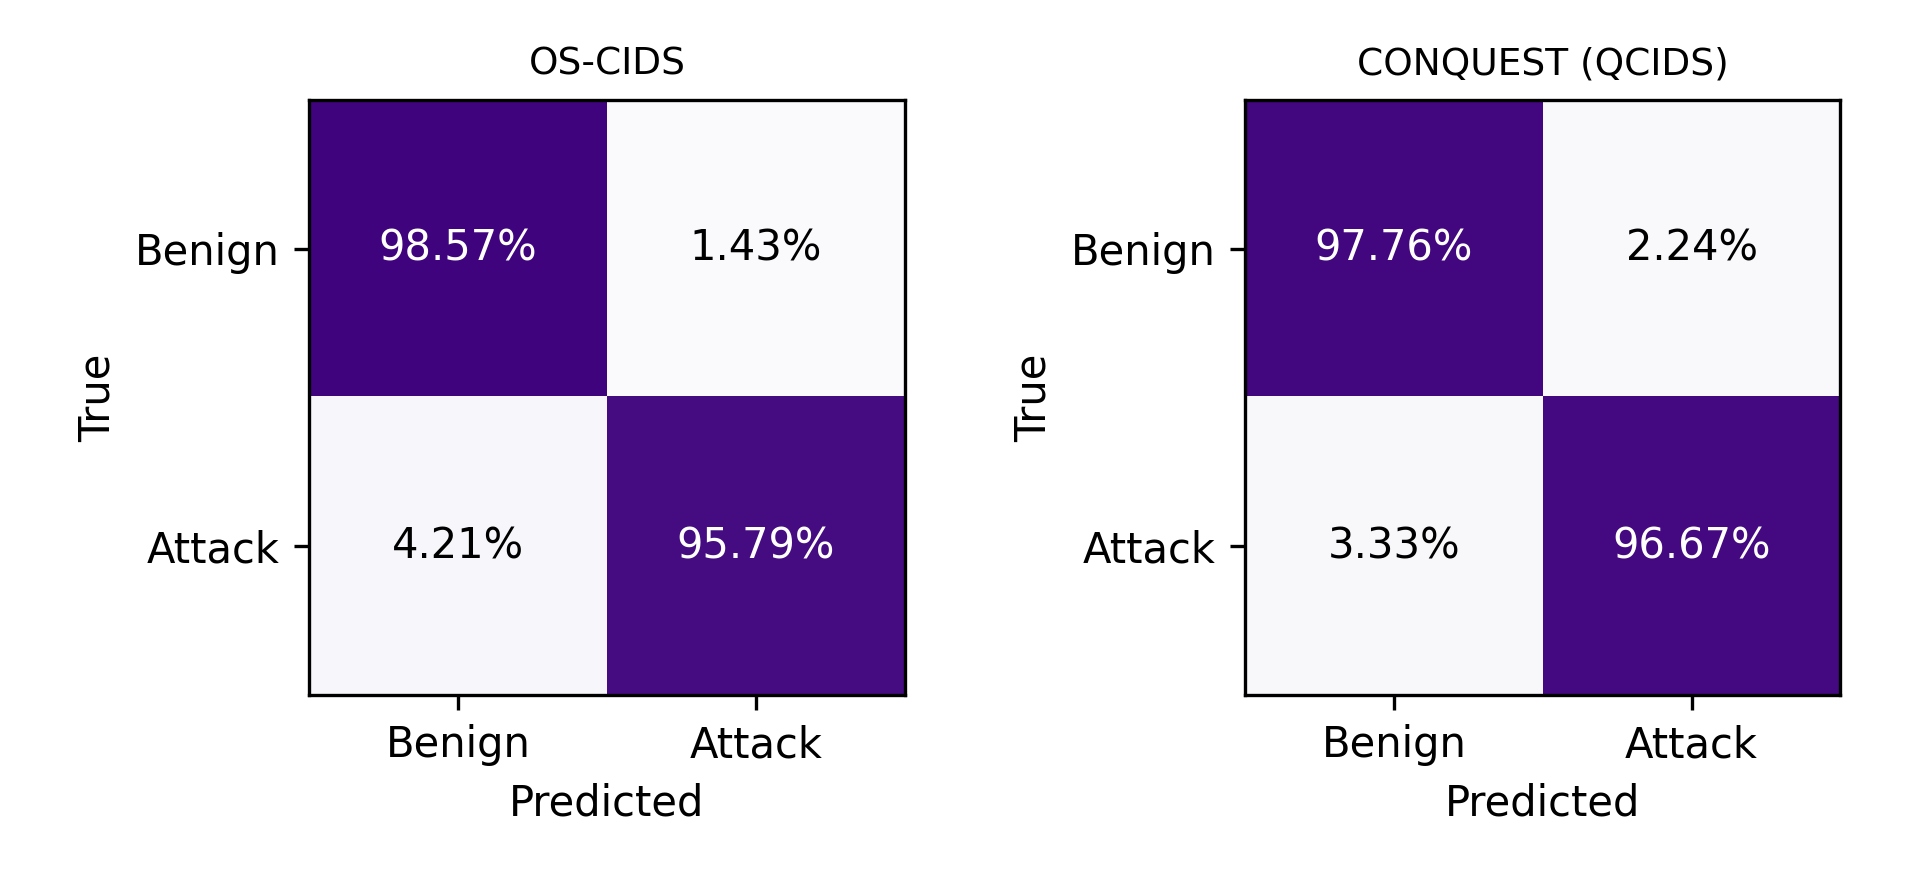
\includegraphics[width=\linewidth]{images/cm_conquest_vs_os.png}
    \caption{\textcolor{black}{Row-normalized confusion matrices of
    OS-CIDS and CONQUEST on the test set, averaged over ten seeds.}}
    
\end{figure}

\setcounter{figure}{4}
\begin{figure}[H]
    \centering
    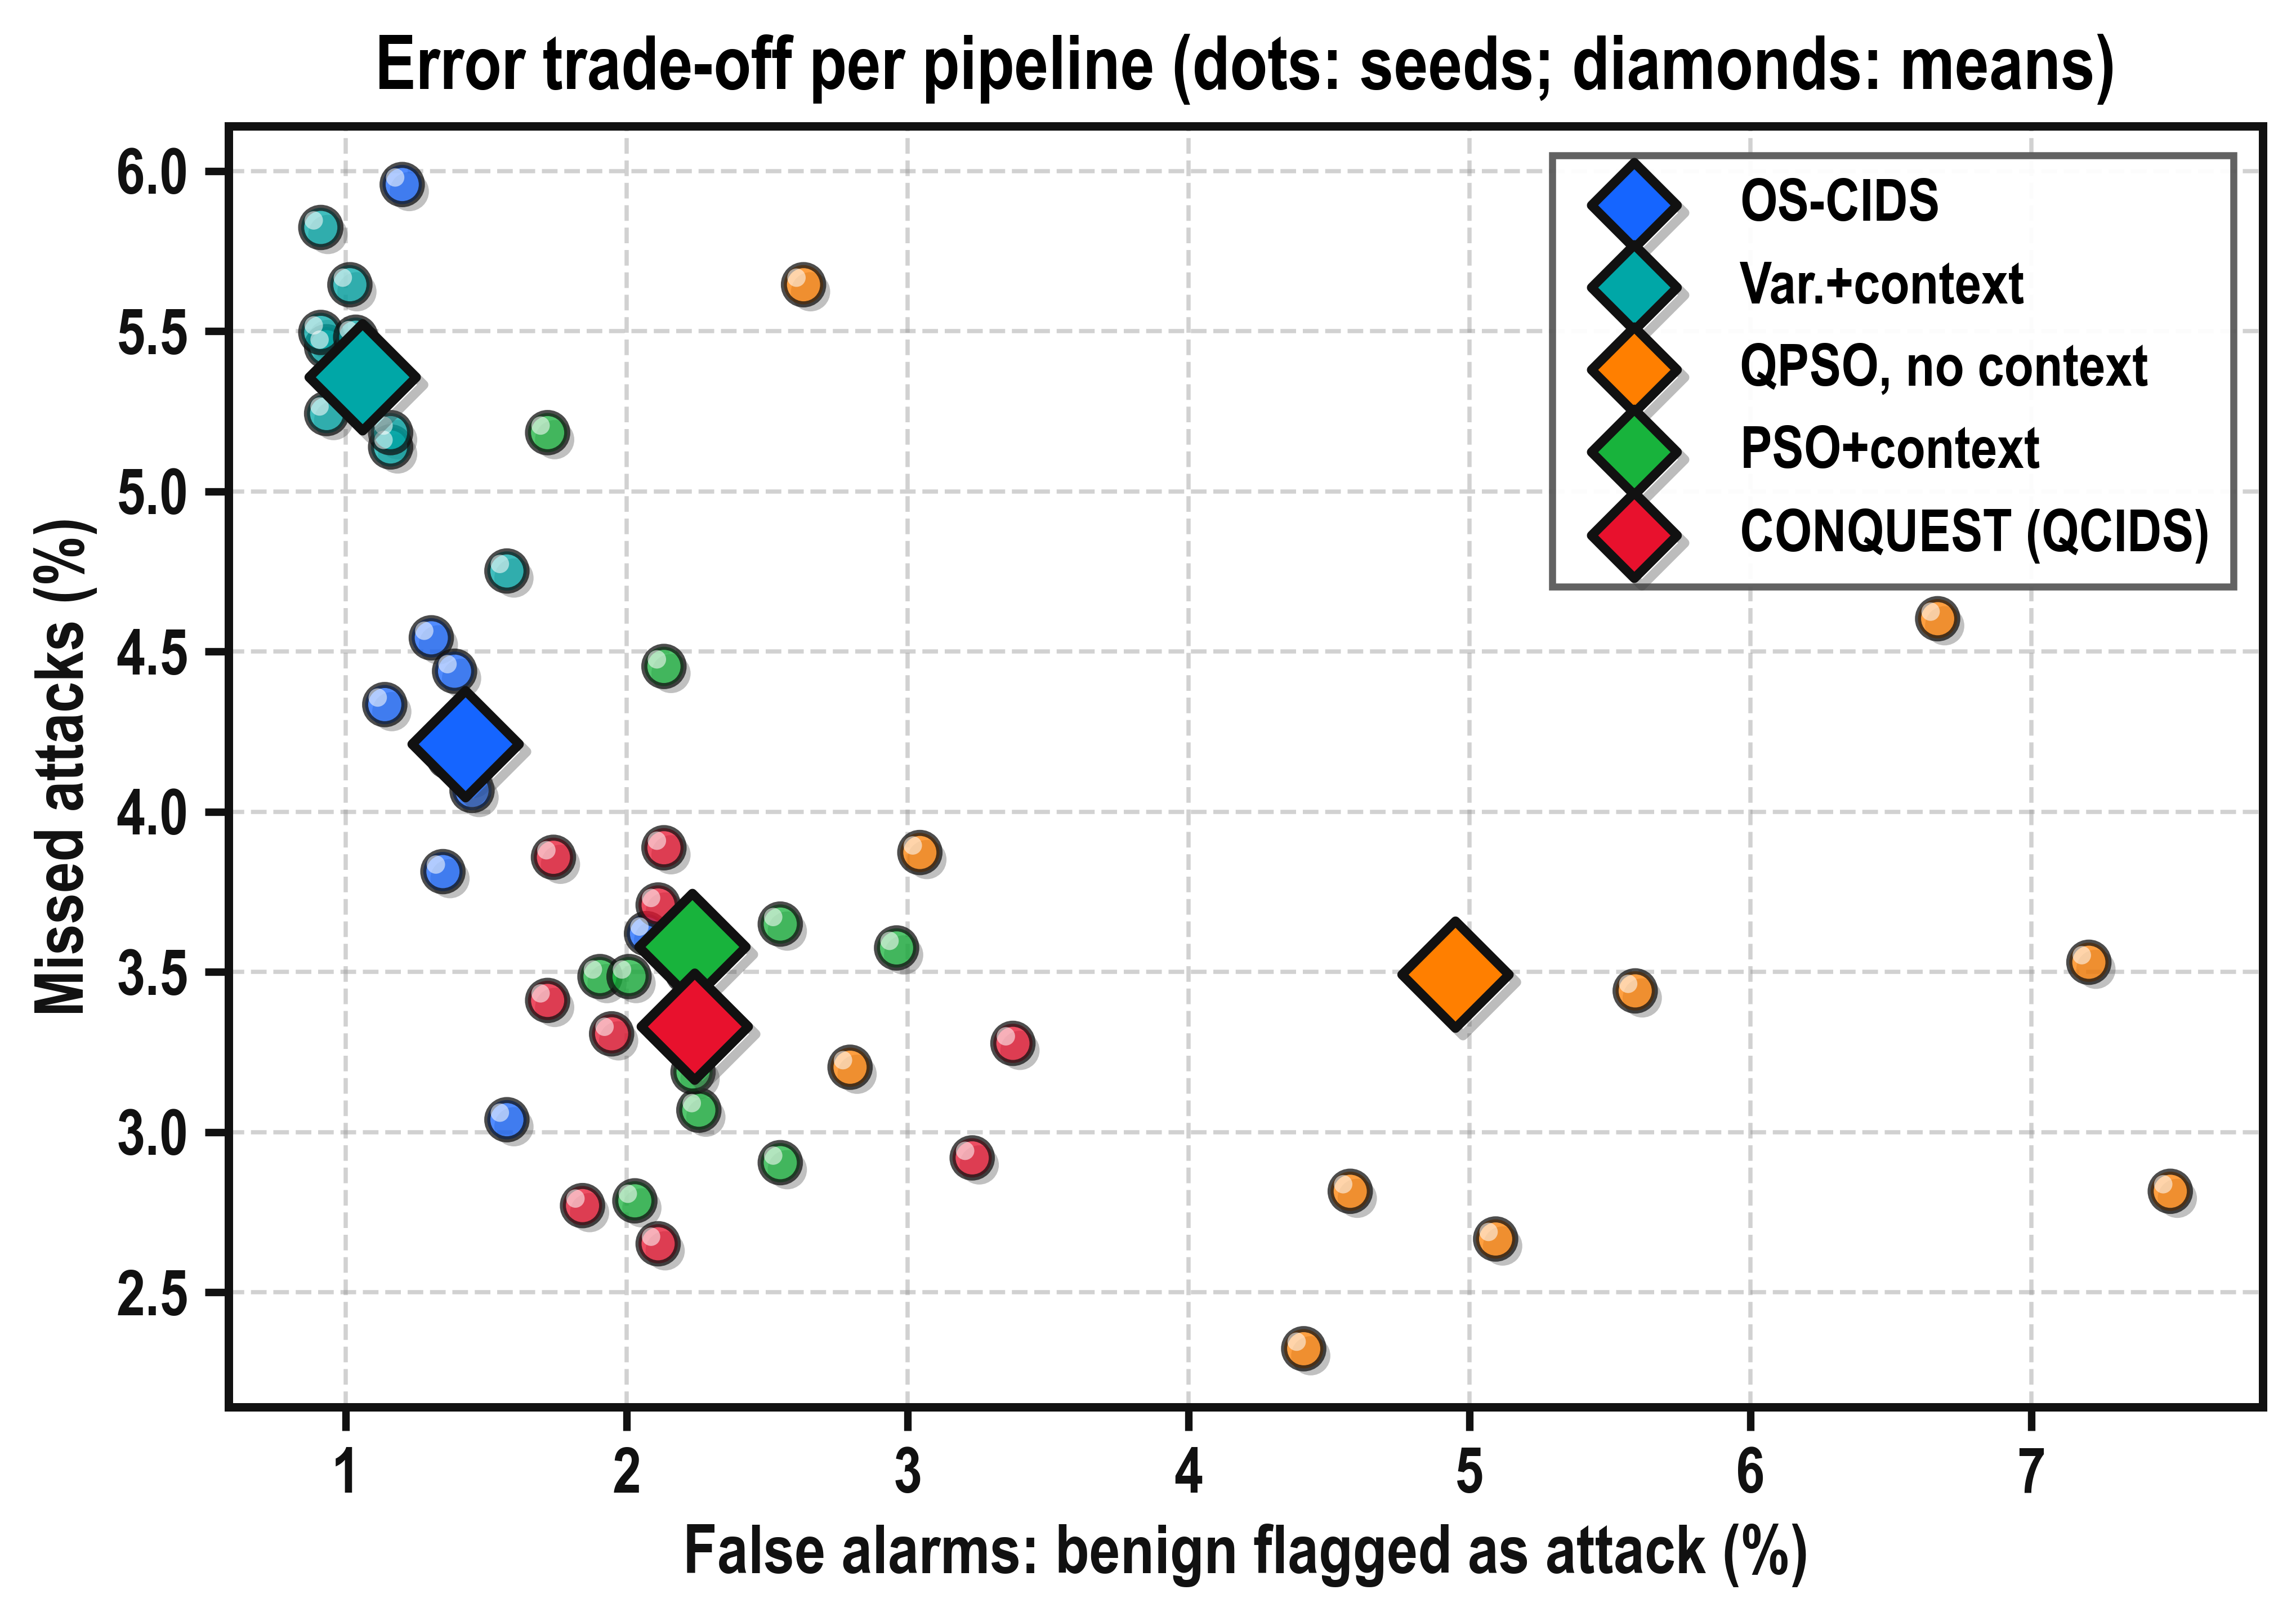
\includegraphics[width=\linewidth]{images/tradeoff_far_md.png}
    \caption{\textcolor{black}{False-alarm rate versus
    missed-attack rate of the five centralized pipelines. Dots:
    individual seeds; diamonds: means.}}
    
\end{figure}

\textcolor{black}{\textbf{Context features versus QPSO.} The
factorial ablation in Table~X separates
the two components, and neither helps on its own. Adding context
features to variance ranking lowers F1 by 0.51\,pp ($p=0.014$),
because variance ranking ignores labels and fills 14 of its 40 slots
with high-variance context counts, displacing informative
packet-length features. Replacing variance ranking by QPSO on static
features alone lowers F1 by 1.07\,pp ($p=0.002$), mainly through more
false alarms. Combined, however, context features and QPSO raise F1
by 1.23\,pp over QPSO alone and by 0.68\,pp over variance ranking with
context (both $p\le0.004$), and their interaction, $+1.74$\,pp
($p=0.002$), is the dominant effect. The gain of CONQUEST therefore
comes from combining context-aware representation with label-aware
selection, which keeps eight context features alongside complementary
static features, as listed in Table~XI.}

\setcounter{table}{9}
\begin{table}[H]
\centering
\scriptsize
\caption{\textcolor{black}{Factorial ablation of context features and QPSO over ten seeds.}}

\color{black}
\setlength{\tabcolsep}{3pt}
\begin{adjustbox}{max width=\linewidth}
\begin{tabular}{lccc}
\hline\toprule
\makecell[l]{F1 / FAR / MD\\(\%)} & \makecell{Variance\\ranking} & \makecell{QPSO\\($Q^{*}{=}6$)} & \makecell{Effect of\\QPSO (pp)} \\
\hline\toprule
Static only & 96.96 / 1.43 / 4.21 & 95.90 / 4.95 / 3.49 & \makecell{$-1.07$\\($p{=}0.002$)} \\
\makecell[l]{Static +\\context} & 96.45 / 1.06 / 5.36 & \textbf{97.13} / 2.24 / \textbf{3.33} & \makecell{$+0.68$\\($p{=}0.002$)} \\
\midrule
\makecell[l]{Effect of\\context (pp)} & \makecell{$-0.51$\\($p{=}0.014$)} & \makecell{$+1.23$\\($p{=}0.004$)} & \makecell{Interaction\\$+1.74$\\($p{=}0.002$)} \\
\hline\toprule
\end{tabular}
\end{adjustbox}
\end{table}

\setcounter{table}{10}
\begin{table}[H]
\centering
\scriptsize
\caption{\textcolor{black}{Deployed consensus mask at Q = 6; context features in italics.}}

\color{black}
\setlength{\tabcolsep}{2.5pt}
\renewcommand{\arraystretch}{1.02}
\begin{adjustbox}{max width=\linewidth}
\begin{tabular}{>{\raggedright\arraybackslash}p{3.0cm}c >{\raggedright\arraybackslash}p{3.0cm}c}
\hline\toprule
Feature & Freq. & Feature & Freq. \\
\hline\toprule
\textit{syn\_frac\_src\_60} & 1.0 & Fwd URG Flags & 0.6 \\
Fwd Packets/\allowbreak s & 0.9 & Packet Length Std & 0.6 \\
\textit{bytes\_rate\_src\_60} & 0.9 & SYN Flag Count & 0.6 \\
Fwd Packet Length Min & 0.8 & RST Flag Count & 0.6 \\
Fwd Header Length & 0.8 & PSH Flag Count & 0.6 \\
Average Packet Size & 0.8 & ACK Flag Count & 0.6 \\
Protocol & 0.7 & URG Flag Count & 0.6 \\
Fwd Packet Length Std & 0.7 & Fwd Segment Size Avg & 0.6 \\
Bwd Packet Length Min & 0.7 & Bwd Packet/\allowbreak Bulk Avg & 0.6 \\
Flow IAT Max & 0.7 & Bwd Bulk Rate Avg & 0.6 \\
Bwd IAT Max & 0.7 & Subflow Bwd Bytes & 0.6 \\
Bwd IAT Min & 0.7 & \textit{n\_flows\_src\_10} & 0.6 \\
Bwd Segment Size Avg & 0.7 & \textit{pkt\_rate\_src\_10} & 0.6 \\
\textit{n\_flows\_src\_60} & 0.7 & \textit{bytes\_rate\_src\_10} & 0.6 \\
\textit{n\_distinct\_dport\_10} & 0.7 & \textit{n\_proto\_switch\_60} & 0.6 \\
Total Length of Fwd Packet & 0.6 & Total Length of Bwd Packet & 0.5 \\
Bwd Packet Length Max & 0.6 & Fwd IAT Mean & 0.5 \\
Flow Packets/\allowbreak s & 0.6 & CWR Flag Count & 0.5 \\
Flow IAT Std & 0.6 & ECE Flag Count & 0.5 \\
Fwd IAT Std & 0.6 & Active Max & 0.5 \\
\hline\toprule
\end{tabular}
\end{adjustbox}
\end{table}

\textcolor{black}{\textbf{Quantum-inspired versus classical
search.} At an equal budget of 620 fitness evaluations, classical
binary PSO reaches a higher trace-ratio fitness than QPSO, 4919
versus 4401, in less time, 76\,s versus 106\,s, while the resulting
detectors are statistically indistinguishable ($p=0.23$ for F1 and
$p=0.49$ for MD). No quantum advantage is therefore claimed. In
CONQUEST, QPSO is one interchangeable instance of label-aware swarm
selection; its practical merits are a single interpretable control
parameter and robustness to that parameter, not superior accuracy.}

\textcolor{black}{\textbf{Choice of selector.} When
missed attacks are the costlier error, as for self-propagating worms,
label-aware selection with context features is preferable. When false
alarms dominate the operational cost, or labelled data are scarce,
variance ranking on static features gives a comparable F1 with the
fewest false alarms among the competitive pipelines, at negligible
cost and without labels. Context features should not be added to a
label-agnostic selector, and with a very tight feature budget,
variance ranking is again preferable, as shown next.}

\textcolor{black}{\textbf{Tight feature budgets.}
Table~XII repeats the selector comparison for $k=40$, 20,
and 10. With $k=40$, QPSO and PSO are equivalent, and QPSO exceeds
variance ranking on all five seeds. With $k=20$, QPSO has the highest
F1, 96.53\%, and the fewest missed attacks, 4.02\% against 4.67\% for
PSO and 5.98\% for variance ranking. With $k=10$, the ordering
reverses: variance ranking reaches 95.94\% F1 and beats QPSO, at
94.00\%, on all five seeds, while PSO reaches 94.34\%. The trace-ratio
fitness rewards low within-class variance, so with few slots the
swarm keeps only 1.6 of the 17 context features on average, whereas
variance ranking keeps five. Label-aware swarm selection therefore
pays off only when the budget leaves room for both context and static
features.}

\setcounter{table}{11}
\begin{table}[H]
\centering
\scriptsize
\caption{\textcolor{black}{Selector comparison under feature budgets of 40, 20, and 10 over five seeds; the consensus mask uses ten. Ctx.: context features kept. Wins: seeds on which QPSO has the higher F1.}}

\color{black}
\setlength{\tabcolsep}{3pt}
\begin{adjustbox}{max width=\linewidth}
\begin{tabular}{clccccc}
\hline\toprule
$k$ & Selector & F1 (\%) & FAR (\%) & MD (\%) & Ctx. & Wins \\
\hline\toprule
\multirow{3}{*}{40} & QPSO & 97.25$\pm$0.22 & 1.95 & 3.35 & 8.2 & -- \\
 & PSO & \textbf{97.28$\pm$0.15} & 2.15 & 3.15 & 6.6 & 3/5 \\
 & Variance & 96.43$\pm$0.15 & 1.07 & 5.38 & 14.0 & 5/5 \\
\midrule
\multirow{3}{*}{20} & QPSO & \textbf{96.53$\pm$0.42} & 2.72 & 4.02 & 1.8 & -- \\
 & PSO & 96.14$\pm$0.87 & 2.75 & 4.67 & 3.2 & 3/5 \\
 & Variance & 96.05$\pm$0.16 & 1.17 & 5.98 & 10.0 & 4/5 \\
\midrule
\multirow{3}{*}{10} & QPSO & 94.00$\pm$0.64 & 3.42 & 7.91 & 1.6 & -- \\
 & PSO & 94.34$\pm$0.51 & 3.73 & 7.08 & 1.4 & 0/5 \\
 & Variance & \textbf{95.94$\pm$0.30} & 1.15 & 6.18 & 5.0 & 0/5 \\
\midrule
40 & Consensus & 97.27$\pm$0.23 & 2.46 & 2.93 & 8.0 & -- \\
\hline\toprule
\end{tabular}
\end{adjustbox}
\end{table}

\textcolor{black}{Table~XIII
and Fig.~6 report the ablation over $Q=1$ to 8 with
ten seeds, re-executing QPSO in every run. Test F1 ranges only from
96.95\% at $Q=4$ to 97.20\% at $Q=1$; this 0.25\,pp spread of the
means is smaller than the average seed-to-seed standard deviation of
0.32\,pp. A Friedman test finds no significant effect of $Q$ on test
F1 ($\chi^2_7=6.07$, $p=0.53$), test AUC ($p=0.63$), or validation F1
($p=0.54$). The pre-declared validation rule selects $Q^{*}=6$, but
$Q^{*}=6$ is statistically indistinguishable from every other setting
(Holm-adjusted Wilcoxon $p\ge0.59$). It is therefore a reproducible
default selected on validation data, not a stability optimum. The two
settings beyond $Q=8$, evaluated with five seeds each, fall in the same band,
with test F1 of 97.30\% at $Q=9$ and 97.25\% at $Q=10$.}

\setcounter{table}{12}
\begin{table}[H]
\centering
\caption{\textcolor{black}{Detection versus QPSO register size over ten seeds; last column: Holm-adjusted p-value against Q = 6.}}

\color{black}
\setlength{\tabcolsep}{3.5pt}
\resizebox{\textwidth}{!}{
\begin{adjustbox}{max width=\linewidth}
\begin{tabular}{ccccccccc}
\hline\toprule
$Q$ & Acc (\%) & F1 (\%) & AUC & MSE & FAR (\%) & MD (\%) & Val.\ F1 (\%) & $p$ vs.\ $Q{=}6$ \\
\hline\toprule
1 & 97.20$\pm$0.23 & 97.20$\pm$0.22 & 0.9926$\pm$0.0009 & 0.0243$\pm$0.0024 & 1.90$\pm$0.29 & 3.45$\pm$0.53 & 95.27$\pm$0.74 & 1.00 \\
2 & 97.08$\pm$0.17 & 97.09$\pm$0.17 & 0.9918$\pm$0.0011 & 0.0253$\pm$0.0019 & 2.19$\pm$0.58 & 3.44$\pm$0.55 & 95.00$\pm$1.58 & 1.00 \\
3 & 96.96$\pm$0.37 & 96.96$\pm$0.37 & 0.9916$\pm$0.0016 & 0.0263$\pm$0.0026 & 2.10$\pm$0.52 & 3.72$\pm$0.85 & 95.56$\pm$1.18 & 0.59 \\
4 & 96.94$\pm$0.49 & 96.95$\pm$0.49 & 0.9917$\pm$0.0021 & 0.0268$\pm$0.0039 & 1.93$\pm$0.29 & 3.87$\pm$0.81 & 95.38$\pm$1.58 & 1.00 \\
5 & 97.05$\pm$0.42 & 97.06$\pm$0.41 & 0.9925$\pm$0.0012 & 0.0249$\pm$0.0026 & 1.92$\pm$0.34 & 3.69$\pm$0.86 & 95.70$\pm$1.24 & 1.00 \\
\textbf{6}$^{*}$ & \textbf{97.13$\pm$0.31} & \textbf{97.13$\pm$0.31} & \textbf{0.9924$\pm$0.0016} & \textbf{0.0246$\pm$0.0028} & \textbf{2.24$\pm$0.58} & \textbf{3.33$\pm$0.44} & \textbf{96.00$\pm$1.04} & -- \\
7 & 97.17$\pm$0.32 & 97.17$\pm$0.32 & 0.9919$\pm$0.0012 & 0.0248$\pm$0.0024 & 2.05$\pm$0.33 & 3.39$\pm$0.69 & 95.75$\pm$0.84 & 1.00 \\
8 & 97.07$\pm$0.26 & 97.08$\pm$0.26 & 0.9918$\pm$0.0008 & 0.0249$\pm$0.0013 & 2.03$\pm$0.34 & 3.57$\pm$0.52 & 95.59$\pm$0.95 & 1.00 \\
\hline\toprule
\end{tabular}
\end{adjustbox}}
\end{table}

\textcolor{black}{Together with Fig.~3,
these results give a consistent picture. $Q$ strongly changes how the
swarm searches, but with 40 of 86 features, including 17 informative
context features, many subsets support equally accurate detectors,
so the classifier is robust to $Q$. In practice, $Q$ needs no fine
tuning: every setting from 1 to 8 yields between 96.95\% and 97.20\%
test F1 over ten seeds, and $Q=9$ and 10 fall in the same band.}

\setcounter{figure}{5}
\begin{figure}[H]
\centering
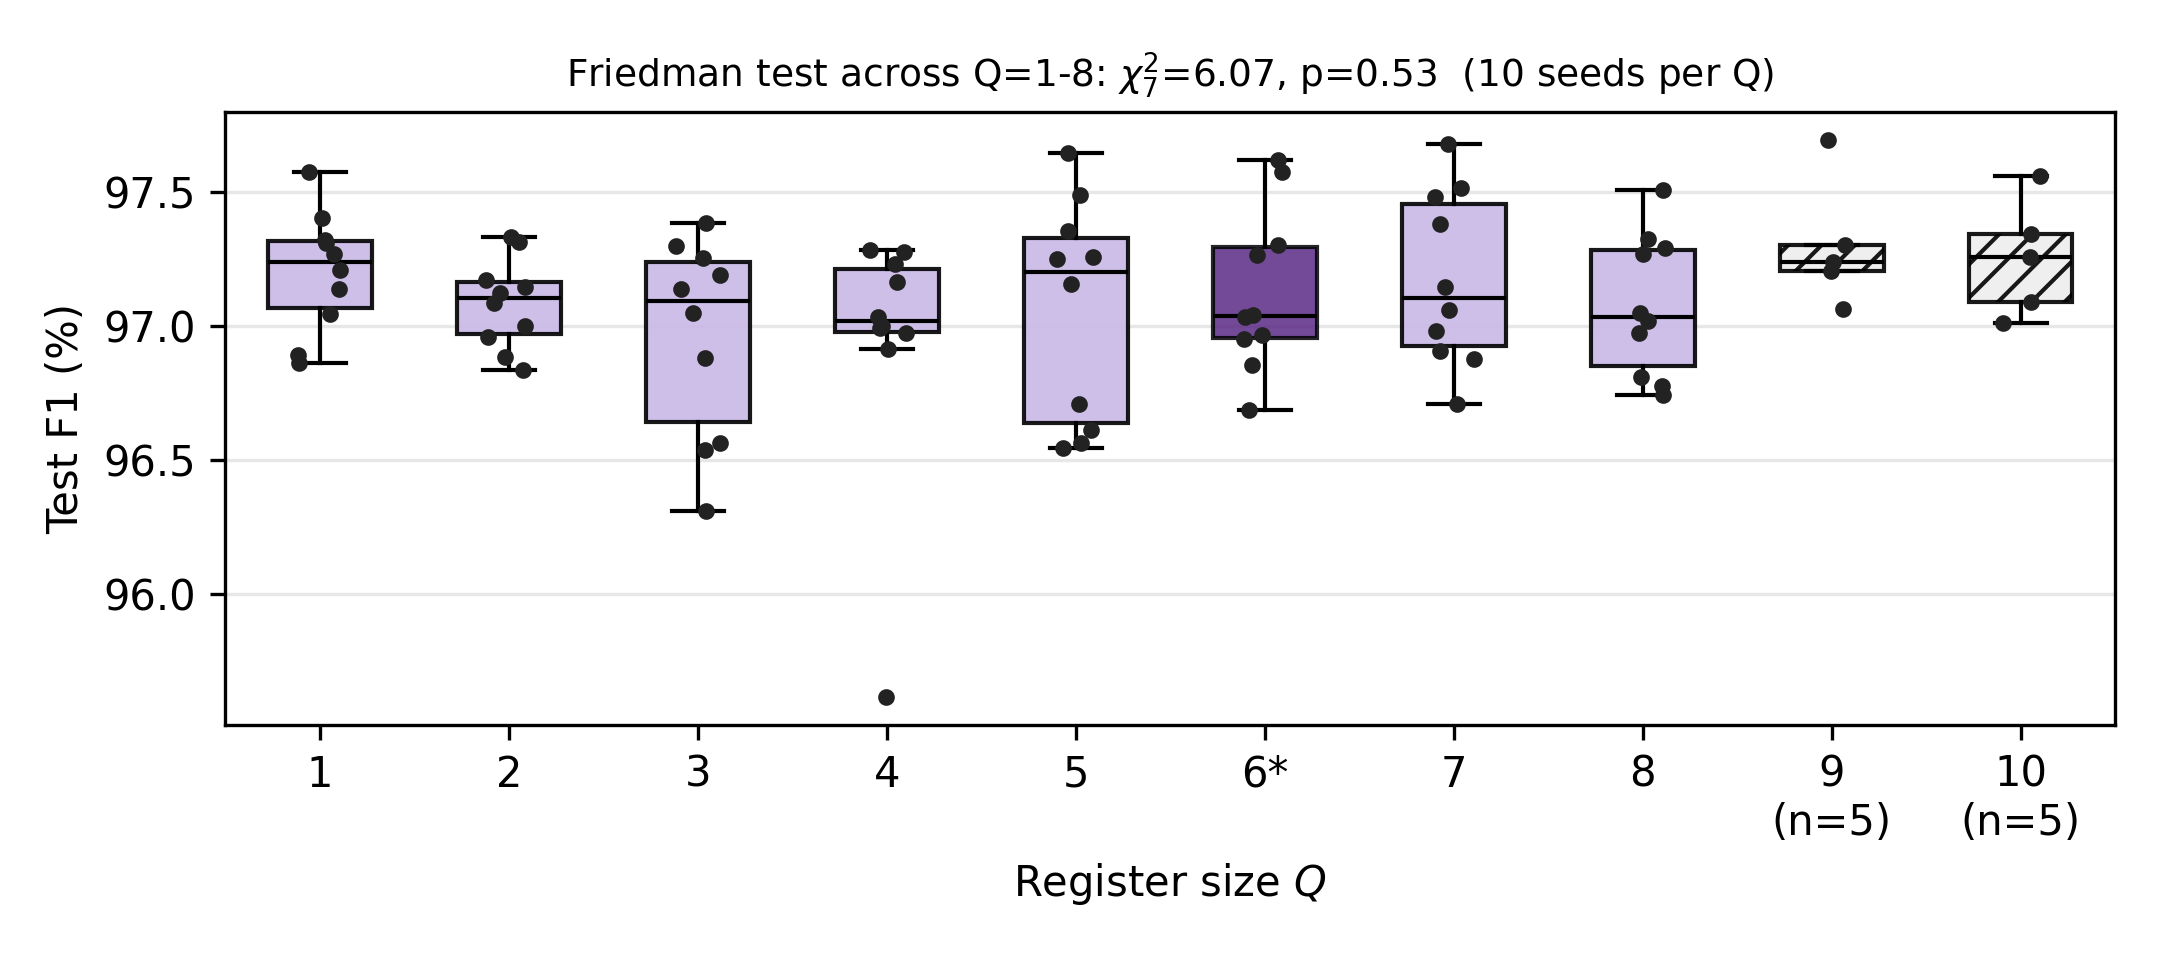
\includegraphics[width=\linewidth]{images/q_ablation_boxplot.png}
\caption{\textcolor{black}{Test F1 versus QPSO register size; hatched boxes use five seeds, the others ten.}}

\end{figure}

\textcolor{red}{\textbf{Search-budget sensitivity.}
Fig.~7(a) shows that the default budget does not fully
converge the search: a larger budget raises the best fitness found for
every $Q$, by 6--21\% at eight times the evaluations. For the trained
runs, the increase is significant, with Friedman $p<10^{-4}$ over the
four budgets and a gain of 387 from $20\times30$ to $40\times60$
(Wilcoxon $p<10^{-6}$). Intermediate $Q$ from 3 to 6 reaches the
highest fitness at every budget, consistent with
Fig.~3. The additional search, however, does not
improve detection, as Table~XIV and
Fig.~7(b) show. Test F1 stays within 96.9--97.3\% in every
cell, with no budget effect (Friedman $p=0.50$; $20\times30$ versus
$40\times60$: mean difference $-0.10$\,pp, Wilcoxon $p=0.15$), and
validation F1 even decreases slightly at $40\times60$ ($-0.6$\,pp,
$p=0.02$). Pushing the training-split fitness further thus mildly
overfits the selection. No degradation at $Q=7$ or 8 appears at any
budget, and the validation-selected $Q$ within 6 to 10 changes with
the budget, to 10, 7, 9, and 9, as expected when no setting is
genuinely better. Larger budgets therefore do not change the conclusion that detection is insensitive to $Q$.
Training detectors for all $Q$ from 1 to 10 at the largest budget of
$40\times60$ with five seeds confirms this: test F1 ranges from
96.89\% to 97.31\%, the Friedman test finds no effect of $Q$
($p=0.46$), and the validation-selected setting moves to $Q=9$. The
default budget of $20\times30$ is retained because it is sufficient
for detection at the lowest cost.}
\end{excerpt}
\setcounter{table}{13}
\begin{table}[H]
\centering
\scriptsize
\caption{\textcolor{red}{Search-budget sensitivity of QPSO over five seeds per cell.}}

\color{red}
\setlength{\tabcolsep}{3pt}
\begin{adjustbox}{max width=\linewidth}
\begin{tabular}{cccccc}
\hline\toprule
$Q$ & $P{\times}I$ & Evals & Fitness & Test F1 (\%) & Val.\ F1 (\%) \\
\hline\toprule
\multirow{4}{*}{6} & 20$\times$30 & 620 & 4412$\pm$334 & 97.25$\pm$0.22 & 96.10$\pm$1.08 \\
 & 40$\times$30 & 1240 & 4872$\pm$291 & 97.20$\pm$0.30 & 95.34$\pm$0.70 \\
 & 20$\times$60 & 1220 & 4856$\pm$317 & 97.12$\pm$0.29 & 94.73$\pm$0.89 \\
 & 40$\times$60 & 2440 & 4953$\pm$141 & 97.01$\pm$0.41 & 94.56$\pm$1.57 \\
\midrule
\multirow{4}{*}{7} & 20$\times$30 & 620 & 4415$\pm$134 & 97.06$\pm$0.29 & 95.74$\pm$1.13 \\
 & 40$\times$30 & 1240 & 4668$\pm$346 & 97.21$\pm$0.38 & 96.23$\pm$1.05 \\
 & 20$\times$60 & 1220 & 4886$\pm$248 & 96.98$\pm$0.36 & 95.72$\pm$1.26 \\
 & 40$\times$60 & 2440 & 4906$\pm$181 & 96.93$\pm$0.38 & 95.58$\pm$0.59 \\
\midrule
\multirow{4}{*}{8} & 20$\times$30 & 620 & 4340$\pm$212 & 97.12$\pm$0.28 & 96.13$\pm$0.48 \\
 & 40$\times$30 & 1240 & 4530$\pm$130 & 96.91$\pm$0.16 & 94.98$\pm$0.36 \\
 & 20$\times$60 & 1220 & 4749$\pm$360 & 97.13$\pm$0.33 & 95.64$\pm$0.52 \\
 & 40$\times$60 & 2440 & 4766$\pm$237 & 97.15$\pm$0.27 & 95.40$\pm$0.73 \\
\midrule
\multirow{4}{*}{9} & 20$\times$30 & 620 & 4435$\pm$222 & 97.30$\pm$0.24 & 95.89$\pm$0.89 \\
 & 40$\times$30 & 1240 & 4423$\pm$208 & 97.13$\pm$0.23 & 95.88$\pm$0.87 \\
 & 20$\times$60 & 1220 & 4473$\pm$399 & 96.97$\pm$0.40 & 95.98$\pm$0.49 \\
 & 40$\times$60 & 2440 & 4625$\pm$165 & 97.14$\pm$0.21 & 95.93$\pm$0.99 \\
\midrule
\multirow{4}{*}{10} & 20$\times$30 & 620 & 4550$\pm$341 & 97.25$\pm$0.22 & 96.18$\pm$0.90 \\
 & 40$\times$30 & 1240 & 4441$\pm$224 & 96.92$\pm$0.25 & 95.46$\pm$0.84 \\
 & 20$\times$60 & 1220 & 4664$\pm$285 & 97.23$\pm$0.11 & 95.80$\pm$1.36 \\
 & 40$\times$60 & 2440 & 4838$\pm$130 & 97.26$\pm$0.13 & 95.56$\pm$1.69 \\
\hline\toprule
\end{tabular}
\end{adjustbox}
\end{table}
\setcounter{figure}{6}
\begin{figure}[H]
\centering
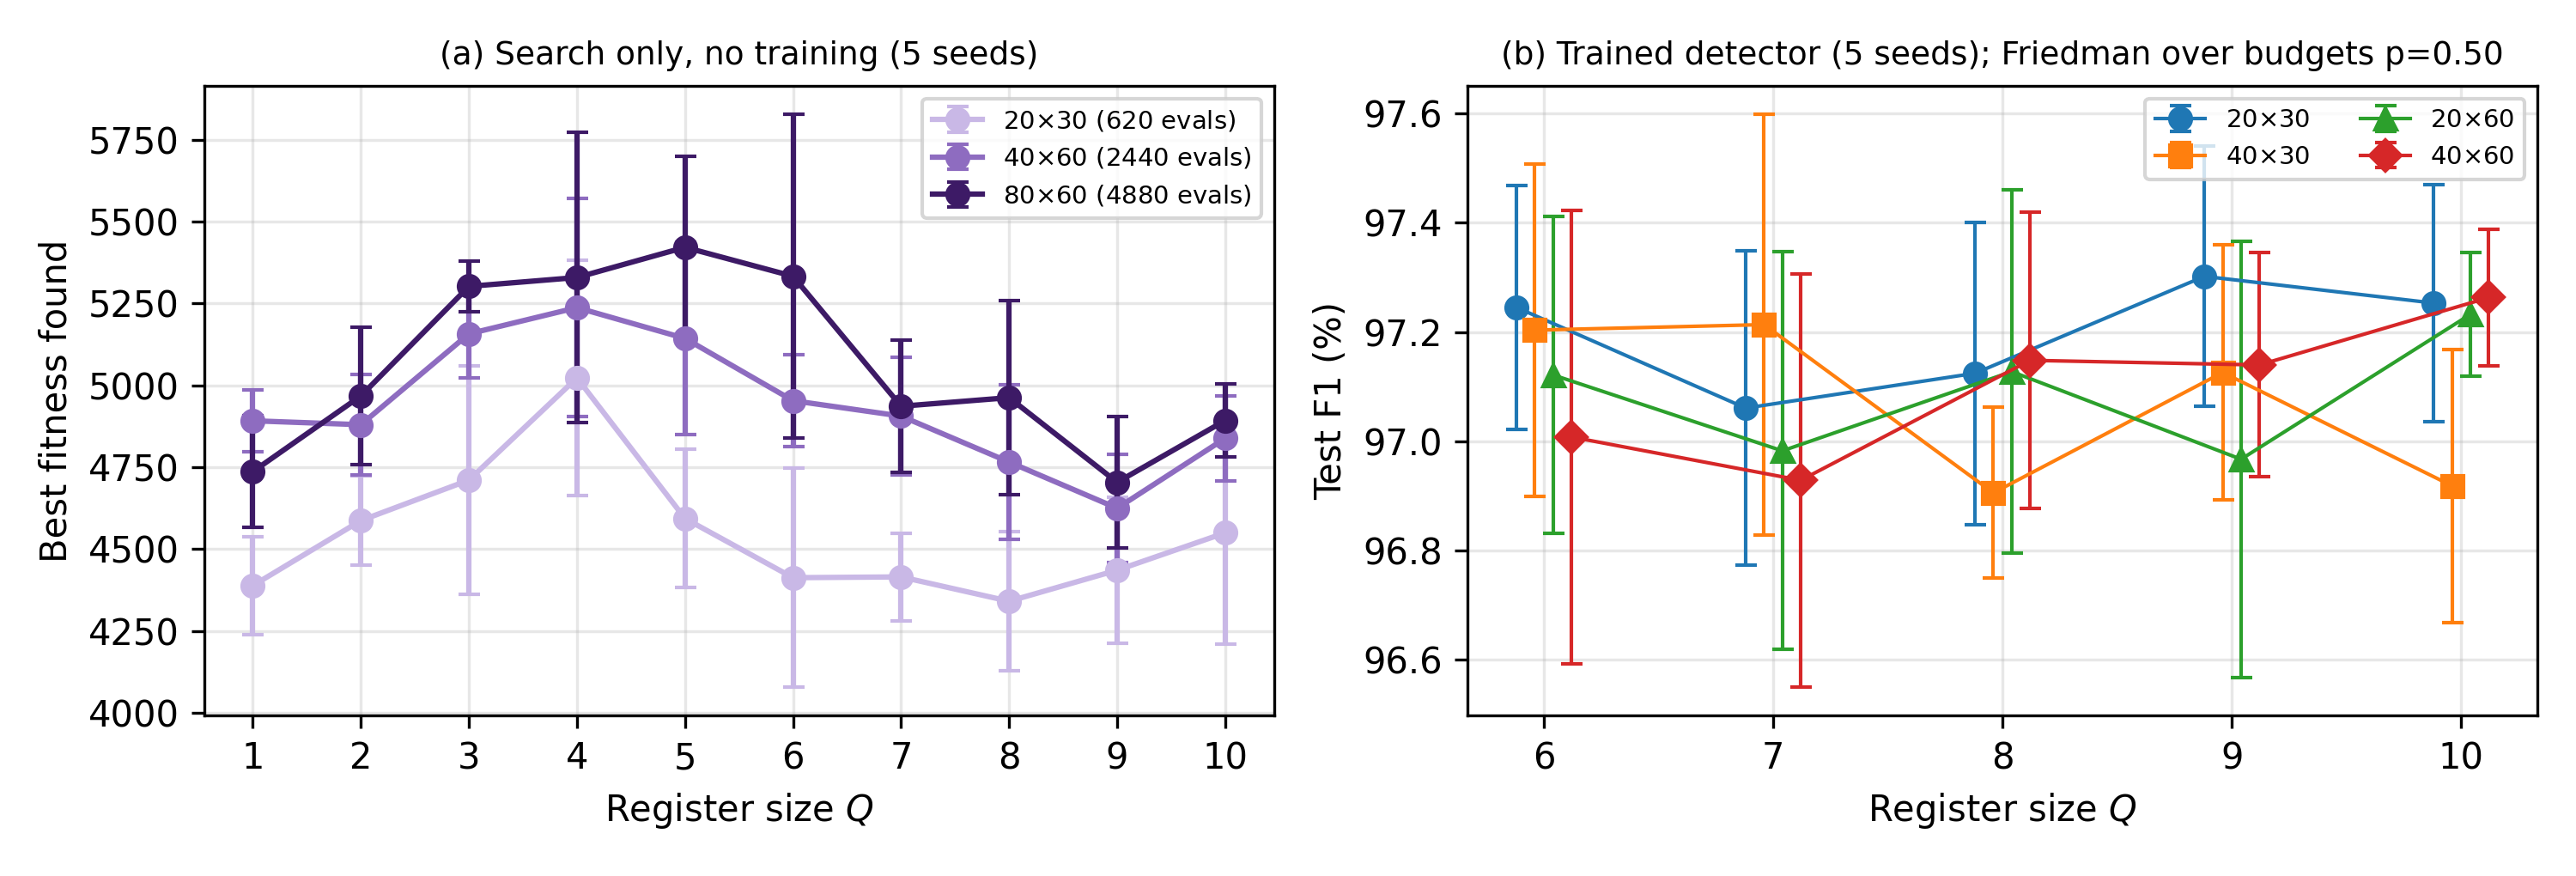
\includegraphics[width=0.9\linewidth]{images/budget_sensitivity.png}
\caption{\textcolor{red}{Search-budget sensitivity: (a)~best fitness of the search alone; (b)~test F1 of trained detectors.}}

\end{figure}

%% ---------------------------------------------------------------------
\review{1.4}{In Section III-B, manuscript pp.~5--6, the final selected feature subset is not reported. The manuscript should provide the selected feature names, the number of retained features $k=\|m^{*}\|_0$, and the consistency of the selected subsets across seeds. Otherwise, the claimed feature compactness and stability cannot be verified.}

\reply We thank the reviewer and now report all three. The number of
retained features is fixed at $k=\|\mathbf{m}^{*}\|_0=40$ of the 86 input
features. Because a single run's mask depends on its seed, the deployed
detector uses a consensus mask, the 40 features selected most often across
the ten QPSO runs; Table~XI lists their names and selection frequencies, and
Fig.~8 shows the selection frequency of every feature for every $Q$.
Consistency is quantified by the mean pairwise Jaccard index, 0.36 at
$Q^{*}=6$ against 0.30 for random subsets, rising to 0.53 against 0.45 when
redundant features (absolute Spearman correlation of at least 0.9) are
grouped. A small core is selected consistently, and the consensus mask
reaches $97.27\pm0.23\%$ F1, statistically equal to the individual masks.
Because $k=40$ keeps 47\% of the features, the claim of compactness has been
withdrawn; a compact operating point at $k=20$ is reported instead, together
with a comparison of selectors at $k=40$, 20, and 10 (Table~XII). Six
CICFlowMeter fields that are constant on the training data are now removed
before selection, so they can no longer occupy mask slots.

\loc{(a) Page 6: Added the consensus mask to Section III-B}
\begin{excerpt}
\mshead{III-B}{Variable-Qubit QPSO Feature Selection}


QPSO learns a sparse binary feature mask
$\mathbf{m}\in\{0,1\}^d$ that gates the normalized input:
\begin{equation}
\tilde{\mathbf{z}} = \mathbf{m}\odot\mathbf{z}_n,\quad
\|\mathbf{m}\|_0 = k \ll d,
\tag{6}
\end{equation}
where $\odot$ denotes element-wise multiplication.
\textcolor{black}{Each of the $P$ particles $i$ holds a
non-negative amplitude vector $\mathbf{a}_i\in\mathbb{R}_{\ge 0}^{d}$
with $\sum_j a_{i,j}=1$, one amplitude per feature, so the particle
dimension is $d$ for every $Q$. The register size $Q$ enters the
search at three points. First, amplitudes are initialized at the
uniform amplitude of a $Q$-qubit register plus Gaussian noise; after
normalization, only the relative perturbation
$\rho(Q)=2^{Q/2}/(Q^{2}+1)$ matters:}
\begin{equation}
\textcolor{black}{a_{i,j}^{(0)} \propto \Bigl|\,2^{-Q/2} +
\tfrac{\xi_{i,j}}{Q^{2}+1}\Bigr|,\quad
\xi_{i,j}\sim\mathcal{N}(0,1).}
\tag{7}
\end{equation}
\textcolor{black}{Second, at iteration $t$, each particle is
rotated toward its personal-best amplitude $\mathbf{a}_i^{\rm pb}$
and the global-best amplitude $\mathbf{a}^{\rm gb}$ by an angle whose
upper bound decreases with $Q$:}
\begin{align}
\textcolor{black}{\phi_t} &\textcolor{black}{= \frac{\pi}{2Q}\Bigl(1-\frac{t}{I}\Bigr),}
\tag{8}\\
\textcolor{black}{\mathbf{a}_i} &\textcolor{black}{\leftarrow \mathbf{a}_i
+ r_1\cos\phi_t\,(\mathbf{a}_i^{\rm pb}-\mathbf{a}_i)
+ r_2\sin\phi_t\,(\mathbf{a}^{\rm gb}-\mathbf{a}_i),}
\tag{9}
\end{align}
\textcolor{black}{with $r_1,r_2\sim\mathcal{U}(0,1)$ drawn per
particle and iteration. Third, each amplitude independently
``collapses'' to a fresh random value with a probability that decays
exponentially in $Q$, and the vector is then renormalized:}
\begin{equation}
\textcolor{black}{a_{i,j} \leftarrow u_{i,j}\sim\mathcal{U}(0,1)
\ \text{w.p. } 2^{-Q},\quad
\mathbf{a}_i \leftarrow |\mathbf{a}_i| / \|\mathbf{a}_i\|_1 .}
\tag{10}
\end{equation}
\textcolor{black}{A mask is obtained by measurement: $k$
distinct feature indices are drawn without replacement with
probabilities $\pi_{i,j}=a_{i,j}^{2}/\sum_{l}a_{i,l}^{2}$, and
$m_{i,j}=1$ for the drawn indices,}
\begin{equation}
\textcolor{black}{\mathbf{m}_i = \textsc{Measure}_k(\boldsymbol{\pi}_i),
\qquad \|\mathbf{m}_i\|_0 = k .}
\tag{11}
\end{equation}
\textcolor{black}{Each run returns $\mathbf{m}^{*}$, the
highest-fitness mask measured during the search, as in standard PSO.
Hence $k$ is a fixed design parameter, set to 40 in all experiments,
and $Q$ shapes \emph{which} $k$ features are found, not how many.
Algorithm~1 summarizes the procedure, and
Table~V lists the constants set by each $Q$.}
\textcolor{red}{Because a single run's mask depends on its
seed, the deployed detector uses a consensus mask
$\mathbf{m}^{*}_{\rm cons}$: the $k$ features selected most often
across the ten QPSO runs at the selected $Q^{*}$, with ties broken by
the summed fitness of the runs that selected them. All ten runs use
$\mathcal{D}_{\rm tr}$ only, so the consensus uses no validation or
test data.}
\end{excerpt}

\loc{(b) Pages 13--15: Added the selected features and their stability to Section IV-A}
\begin{excerpt}
\mshead{IV-A}{Centralized Cyberworm Detection Performance}


Table~IX reports centralized detection
performance \textcolor{black}{of five pipelines that share the
classifier, the data protocol, and $k=40$. They differ only in the
feature representation, static only or static plus context, and in
the selector: variance ranking, classical PSO, or QPSO. They are named
OS-CIDS (variance ranking, static only), Var.+context (variance
ranking, static plus context), QPSO, no context, PSO+context
(classical PSO, static plus context), and CONQUEST (QPSO, static plus
context). All metrics
are computed on $\mathcal{D}_{\rm te}$, which contains 41.8\% benign
and 58.2\% attack windows, and averaged over ten seeds; accuracy and
weighted F1 nearly coincide because both classes are well
represented.}

\setcounter{table}{8}
\begin{table}[H]
\centering
\caption{\textcolor{black}{Centralized detection over ten seeds, with Wilcoxon p-values against CONQUEST. \textsuperscript{\textdagger}Conference result~{[9]}, not directly comparable.}}

\color{black}
\setlength{\tabcolsep}{3pt}
\resizebox{\textwidth}{!}{
\begin{adjustbox}{max width=\linewidth}
\begin{tabular}{lccccccccc}
\hline\toprule
\textbf{Pipeline} & Acc (\%) & F1 (\%) & AUC & MSE & FAR (\%) & MD (\%) & $p$ (F1) & $p$ (MD) & Selection (s) \\
\hline\toprule
S-CIDS~{[9]}\textsuperscript{\textdagger} & 85.14 & 80.62 & -- & -- & -- & -- & -- & -- & -- \\
\midrule
OS-CIDS & 96.95$\pm$0.39 & 96.96$\pm$0.39 & 0.9944$\pm$0.0011 & 0.0245$\pm$0.0025 & 1.43$\pm$0.26 & 4.21$\pm$0.76 & 0.322 & 0.004 & 0.0 \\
Var.+context & 96.44$\pm$0.11 & 96.45$\pm$0.11 & 0.9925$\pm$0.0007 & 0.0291$\pm$0.0015 & 1.06$\pm$0.20 & 5.36$\pm$0.30 & 0.002 & 0.002 & 0.1 \\
QPSO, no context & 95.90$\pm$0.83 & 95.90$\pm$0.83 & 0.9879$\pm$0.0030 & 0.0329$\pm$0.0060 & 4.95$\pm$1.80 & 3.49$\pm$1.00 & 0.004 & 0.824 & 68.0 \\
PSO+context & 96.98$\pm$0.40 & 96.99$\pm$0.39 & 0.9918$\pm$0.0018 & 0.0254$\pm$0.0031 & 2.23$\pm$0.37 & 3.58$\pm$0.73 & 0.232 & 0.492 & 75.6 \\
\textbf{CONQUEST (QCIDS)} & \textbf{97.13$\pm$0.31} & \textbf{97.13$\pm$0.31} & \textbf{0.9924$\pm$0.0016} & \textbf{0.0246$\pm$0.0028} & \textbf{2.24$\pm$0.58} & \textbf{3.33$\pm$0.44} & -- & -- & 105.9 \\
\hline\toprule
\end{tabular}
\end{adjustbox}}
\end{table}

\textbf{S-CIDS}, the conference baseline~{[9]},
achieves 85.14\% accuracy and 80.62\% F1. \textcolor{black}{This single-run result was
obtained with a random split of pooled data and is quoted for
reference only; it is not comparable with the leakage-free results
below.}

\textcolor{black}{\textbf{Overall comparison.}
CONQUEST reaches the highest mean F1, $97.13\pm0.31\%$, and the lowest
missed-attack rate, 3.33\%. Its F1, however, is not significantly
higher than that of OS-CIDS, 96.96\% with Wilcoxon $p=0.32$, or of
classical PSO with context features, 96.99\% with $p=0.23$. The
pipelines differ instead in the type of error they make. CONQUEST
misses significantly fewer attacks than OS-CIDS, 3.33\% versus 4.21\%
with $p=0.004$, but raises significantly more false alarms, 2.24\%
versus 1.43\% with $p=0.002$, as the confusion matrices in
Fig.~4 show. All pipelines except QPSO without
context features have nearly identical AUC, 0.992--0.994, and thus
rank attacks above benign traffic equally well.
Fig.~5 shows the resulting trade-off between
false alarms and missed attacks.}

\setcounter{figure}{3}
\begin{figure}[H]
    \centering
    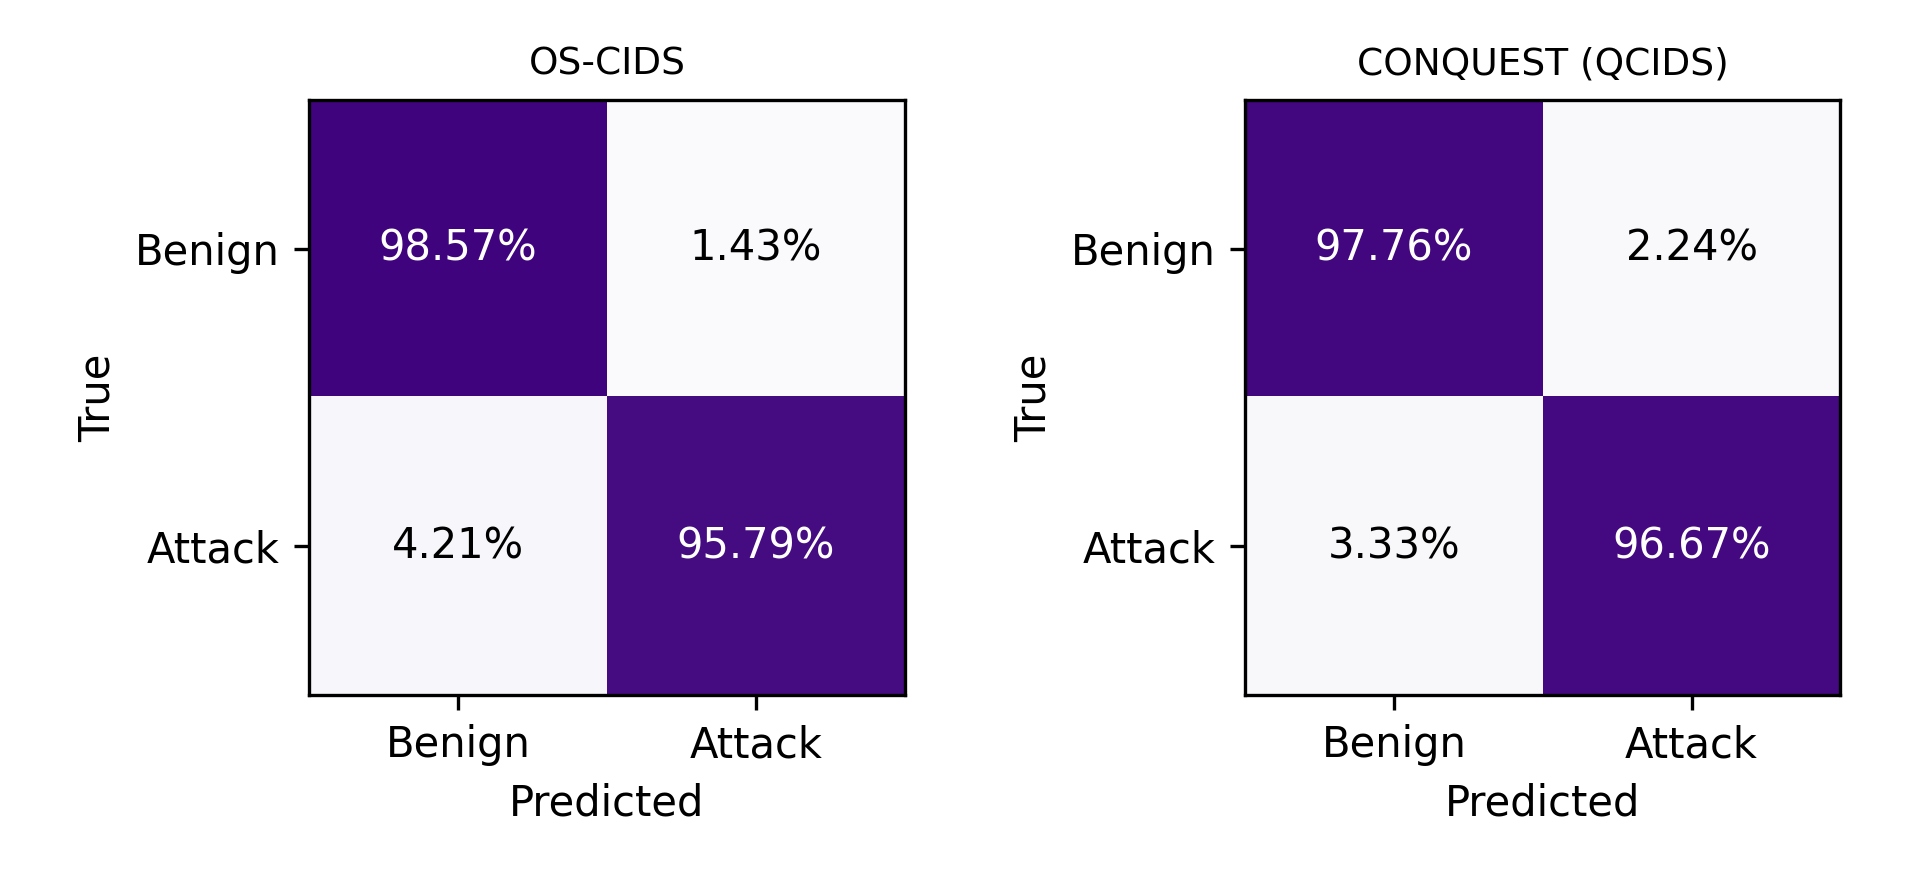
\includegraphics[width=\linewidth]{images/cm_conquest_vs_os.png}
    \caption{\textcolor{black}{Row-normalized confusion matrices of
    OS-CIDS and CONQUEST on the test set, averaged over ten seeds.}}
    
\end{figure}

\setcounter{figure}{4}
\begin{figure}[H]
    \centering
    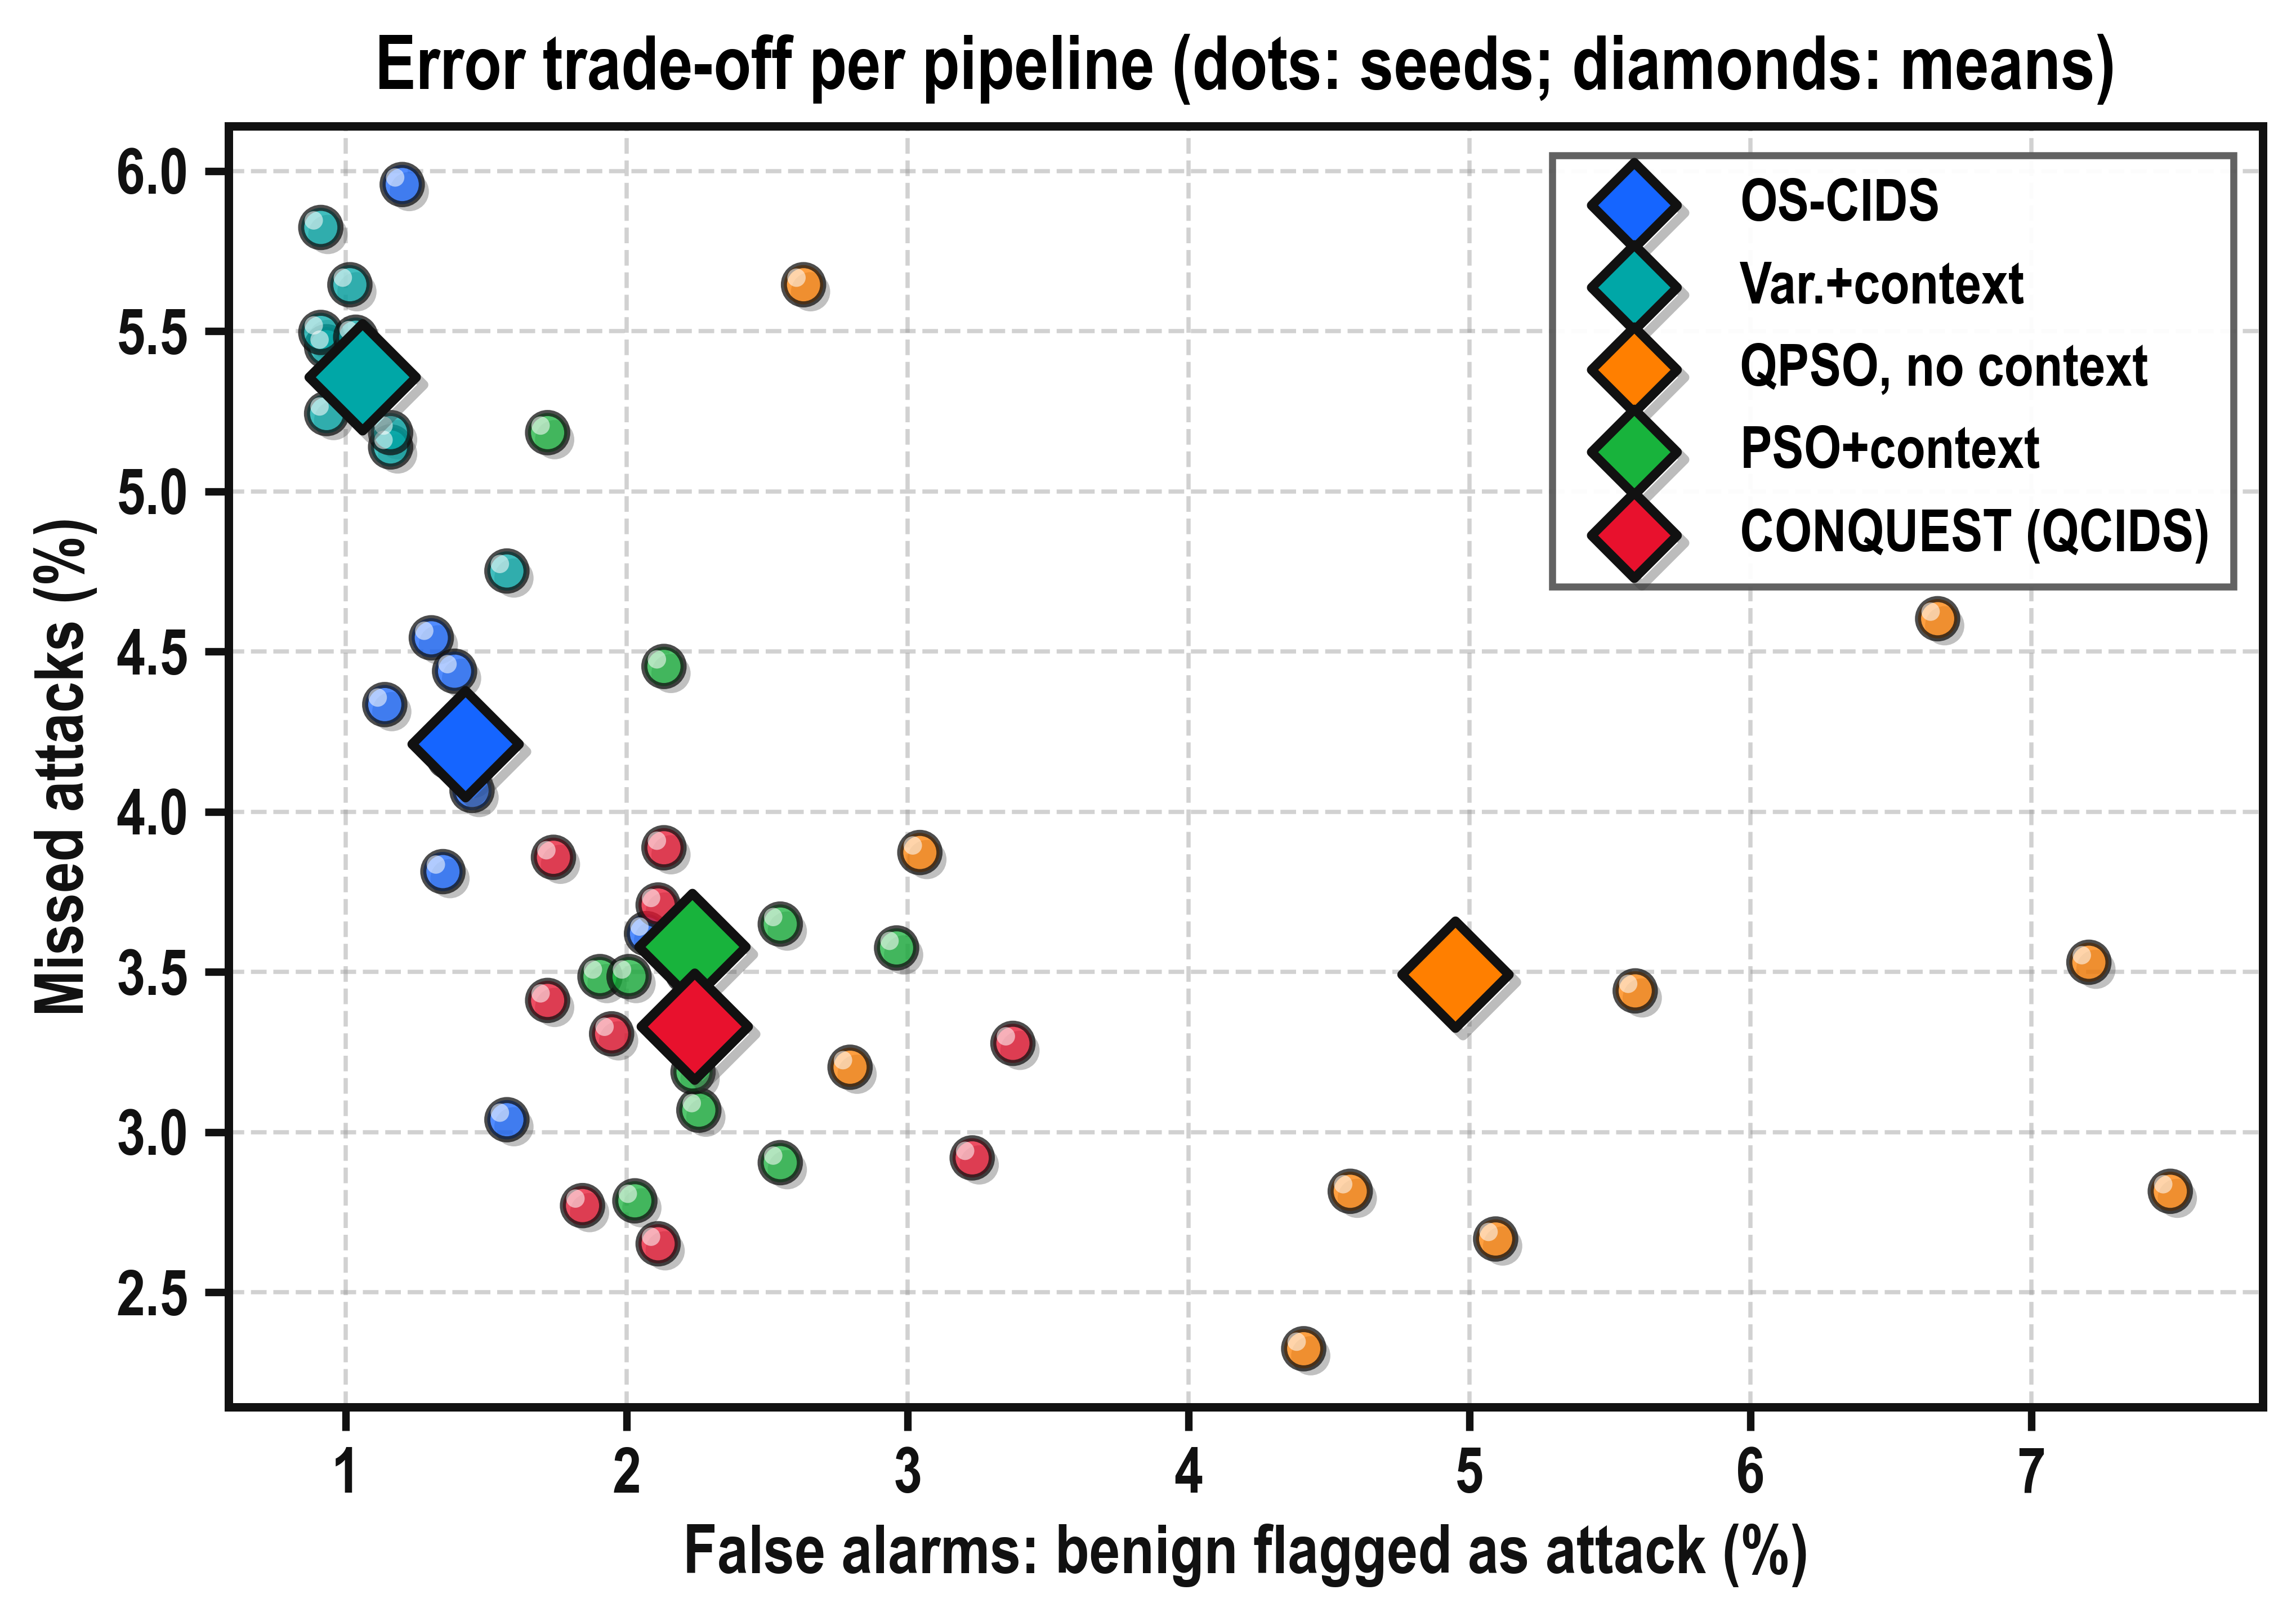
\includegraphics[width=\linewidth]{images/tradeoff_far_md.png}
    \caption{\textcolor{black}{False-alarm rate versus
    missed-attack rate of the five centralized pipelines. Dots:
    individual seeds; diamonds: means.}}
    
\end{figure}

\textcolor{black}{\textbf{Context features versus QPSO.} The
factorial ablation in Table~X separates
the two components, and neither helps on its own. Adding context
features to variance ranking lowers F1 by 0.51\,pp ($p=0.014$),
because variance ranking ignores labels and fills 14 of its 40 slots
with high-variance context counts, displacing informative
packet-length features. Replacing variance ranking by QPSO on static
features alone lowers F1 by 1.07\,pp ($p=0.002$), mainly through more
false alarms. Combined, however, context features and QPSO raise F1
by 1.23\,pp over QPSO alone and by 0.68\,pp over variance ranking with
context (both $p\le0.004$), and their interaction, $+1.74$\,pp
($p=0.002$), is the dominant effect. The gain of CONQUEST therefore
comes from combining context-aware representation with label-aware
selection, which keeps eight context features alongside complementary
static features, as listed in Table~XI.}

\setcounter{table}{9}
\begin{table}[H]
\centering
\scriptsize
\caption{\textcolor{black}{Factorial ablation of context features and QPSO over ten seeds.}}

\color{black}
\setlength{\tabcolsep}{3pt}
\begin{adjustbox}{max width=\linewidth}
\begin{tabular}{lccc}
\hline\toprule
\makecell[l]{F1 / FAR / MD\\(\%)} & \makecell{Variance\\ranking} & \makecell{QPSO\\($Q^{*}{=}6$)} & \makecell{Effect of\\QPSO (pp)} \\
\hline\toprule
Static only & 96.96 / 1.43 / 4.21 & 95.90 / 4.95 / 3.49 & \makecell{$-1.07$\\($p{=}0.002$)} \\
\makecell[l]{Static +\\context} & 96.45 / 1.06 / 5.36 & \textbf{97.13} / 2.24 / \textbf{3.33} & \makecell{$+0.68$\\($p{=}0.002$)} \\
\midrule
\makecell[l]{Effect of\\context (pp)} & \makecell{$-0.51$\\($p{=}0.014$)} & \makecell{$+1.23$\\($p{=}0.004$)} & \makecell{Interaction\\$+1.74$\\($p{=}0.002$)} \\
\hline\toprule
\end{tabular}
\end{adjustbox}
\end{table}

\setcounter{table}{10}
\begin{table}[H]
\centering
\scriptsize
\caption{\textcolor{red}{Deployed consensus mask at Q = 6; context features in italics.}}

\color{red}
\setlength{\tabcolsep}{2.5pt}
\renewcommand{\arraystretch}{1.02}
\begin{adjustbox}{max width=\linewidth}
\begin{tabular}{>{\raggedright\arraybackslash}p{3.0cm}c >{\raggedright\arraybackslash}p{3.0cm}c}
\hline\toprule
Feature & Freq. & Feature & Freq. \\
\hline\toprule
\textit{syn\_frac\_src\_60} & 1.0 & Fwd URG Flags & 0.6 \\
Fwd Packets/\allowbreak s & 0.9 & Packet Length Std & 0.6 \\
\textit{bytes\_rate\_src\_60} & 0.9 & SYN Flag Count & 0.6 \\
Fwd Packet Length Min & 0.8 & RST Flag Count & 0.6 \\
Fwd Header Length & 0.8 & PSH Flag Count & 0.6 \\
Average Packet Size & 0.8 & ACK Flag Count & 0.6 \\
Protocol & 0.7 & URG Flag Count & 0.6 \\
Fwd Packet Length Std & 0.7 & Fwd Segment Size Avg & 0.6 \\
Bwd Packet Length Min & 0.7 & Bwd Packet/\allowbreak Bulk Avg & 0.6 \\
Flow IAT Max & 0.7 & Bwd Bulk Rate Avg & 0.6 \\
Bwd IAT Max & 0.7 & Subflow Bwd Bytes & 0.6 \\
Bwd IAT Min & 0.7 & \textit{n\_flows\_src\_10} & 0.6 \\
Bwd Segment Size Avg & 0.7 & \textit{pkt\_rate\_src\_10} & 0.6 \\
\textit{n\_flows\_src\_60} & 0.7 & \textit{bytes\_rate\_src\_10} & 0.6 \\
\textit{n\_distinct\_dport\_10} & 0.7 & \textit{n\_proto\_switch\_60} & 0.6 \\
Total Length of Fwd Packet & 0.6 & Total Length of Bwd Packet & 0.5 \\
Bwd Packet Length Max & 0.6 & Fwd IAT Mean & 0.5 \\
Flow Packets/\allowbreak s & 0.6 & CWR Flag Count & 0.5 \\
Flow IAT Std & 0.6 & ECE Flag Count & 0.5 \\
Fwd IAT Std & 0.6 & Active Max & 0.5 \\
\hline\toprule
\end{tabular}
\end{adjustbox}
\end{table}

\textcolor{black}{\textbf{Quantum-inspired versus classical
search.} At an equal budget of 620 fitness evaluations, classical
binary PSO reaches a higher trace-ratio fitness than QPSO, 4919
versus 4401, in less time, 76\,s versus 106\,s, while the resulting
detectors are statistically indistinguishable ($p=0.23$ for F1 and
$p=0.49$ for MD). No quantum advantage is therefore claimed. In
CONQUEST, QPSO is one interchangeable instance of label-aware swarm
selection; its practical merits are a single interpretable control
parameter and robustness to that parameter, not superior accuracy.}

\textcolor{black}{\textbf{Choice of selector.} When
missed attacks are the costlier error, as for self-propagating worms,
label-aware selection with context features is preferable. When false
alarms dominate the operational cost, or labelled data are scarce,
variance ranking on static features gives a comparable F1 with the
fewest false alarms among the competitive pipelines, at negligible
cost and without labels. Context features should not be added to a
label-agnostic selector, and with a very tight feature budget,
variance ranking is again preferable, as shown next.}

\textcolor{black}{\textbf{Tight feature budgets.}
Table~XII repeats the selector comparison for $k=40$, 20,
and 10. With $k=40$, QPSO and PSO are equivalent, and QPSO exceeds
variance ranking on all five seeds. With $k=20$, QPSO has the highest
F1, 96.53\%, and the fewest missed attacks, 4.02\% against 4.67\% for
PSO and 5.98\% for variance ranking. With $k=10$, the ordering
reverses: variance ranking reaches 95.94\% F1 and beats QPSO, at
94.00\%, on all five seeds, while PSO reaches 94.34\%. The trace-ratio
fitness rewards low within-class variance, so with few slots the
swarm keeps only 1.6 of the 17 context features on average, whereas
variance ranking keeps five. Label-aware swarm selection therefore
pays off only when the budget leaves room for both context and static
features.}

\setcounter{table}{11}
\begin{table}[H]
\centering
\scriptsize
\caption{\textcolor{red}{Selector comparison under feature budgets of 40, 20, and 10 over five seeds; the consensus mask uses ten. Ctx.: context features kept. Wins: seeds on which QPSO has the higher F1.}}

\color{red}
\setlength{\tabcolsep}{3pt}
\begin{adjustbox}{max width=\linewidth}
\begin{tabular}{clccccc}
\hline\toprule
$k$ & Selector & F1 (\%) & FAR (\%) & MD (\%) & Ctx. & Wins \\
\hline\toprule
\multirow{3}{*}{40} & QPSO & 97.25$\pm$0.22 & 1.95 & 3.35 & 8.2 & -- \\
 & PSO & \textbf{97.28$\pm$0.15} & 2.15 & 3.15 & 6.6 & 3/5 \\
 & Variance & 96.43$\pm$0.15 & 1.07 & 5.38 & 14.0 & 5/5 \\
\midrule
\multirow{3}{*}{20} & QPSO & \textbf{96.53$\pm$0.42} & 2.72 & 4.02 & 1.8 & -- \\
 & PSO & 96.14$\pm$0.87 & 2.75 & 4.67 & 3.2 & 3/5 \\
 & Variance & 96.05$\pm$0.16 & 1.17 & 5.98 & 10.0 & 4/5 \\
\midrule
\multirow{3}{*}{10} & QPSO & 94.00$\pm$0.64 & 3.42 & 7.91 & 1.6 & -- \\
 & PSO & 94.34$\pm$0.51 & 3.73 & 7.08 & 1.4 & 0/5 \\
 & Variance & \textbf{95.94$\pm$0.30} & 1.15 & 6.18 & 5.0 & 0/5 \\
\midrule
40 & Consensus & 97.27$\pm$0.23 & 2.46 & 2.93 & 8.0 & -- \\
\hline\toprule
\end{tabular}
\end{adjustbox}
\end{table}

\textcolor{black}{Table~XIII
and Fig.~6 report the ablation over $Q=1$ to 8 with
ten seeds, re-executing QPSO in every run. Test F1 ranges only from
96.95\% at $Q=4$ to 97.20\% at $Q=1$; this 0.25\,pp spread of the
means is smaller than the average seed-to-seed standard deviation of
0.32\,pp. A Friedman test finds no significant effect of $Q$ on test
F1 ($\chi^2_7=6.07$, $p=0.53$), test AUC ($p=0.63$), or validation F1
($p=0.54$). The pre-declared validation rule selects $Q^{*}=6$, but
$Q^{*}=6$ is statistically indistinguishable from every other setting
(Holm-adjusted Wilcoxon $p\ge0.59$). It is therefore a reproducible
default selected on validation data, not a stability optimum. The two
settings beyond $Q=8$, evaluated with five seeds each, fall in the same band,
with test F1 of 97.30\% at $Q=9$ and 97.25\% at $Q=10$.}

\setcounter{table}{12}
\begin{table}[H]
\centering
\caption{\textcolor{black}{Detection versus QPSO register size over ten seeds; last column: Holm-adjusted p-value against Q = 6.}}

\color{black}
\setlength{\tabcolsep}{3.5pt}
\resizebox{\textwidth}{!}{
\begin{adjustbox}{max width=\linewidth}
\begin{tabular}{ccccccccc}
\hline\toprule
$Q$ & Acc (\%) & F1 (\%) & AUC & MSE & FAR (\%) & MD (\%) & Val.\ F1 (\%) & $p$ vs.\ $Q{=}6$ \\
\hline\toprule
1 & 97.20$\pm$0.23 & 97.20$\pm$0.22 & 0.9926$\pm$0.0009 & 0.0243$\pm$0.0024 & 1.90$\pm$0.29 & 3.45$\pm$0.53 & 95.27$\pm$0.74 & 1.00 \\
2 & 97.08$\pm$0.17 & 97.09$\pm$0.17 & 0.9918$\pm$0.0011 & 0.0253$\pm$0.0019 & 2.19$\pm$0.58 & 3.44$\pm$0.55 & 95.00$\pm$1.58 & 1.00 \\
3 & 96.96$\pm$0.37 & 96.96$\pm$0.37 & 0.9916$\pm$0.0016 & 0.0263$\pm$0.0026 & 2.10$\pm$0.52 & 3.72$\pm$0.85 & 95.56$\pm$1.18 & 0.59 \\
4 & 96.94$\pm$0.49 & 96.95$\pm$0.49 & 0.9917$\pm$0.0021 & 0.0268$\pm$0.0039 & 1.93$\pm$0.29 & 3.87$\pm$0.81 & 95.38$\pm$1.58 & 1.00 \\
5 & 97.05$\pm$0.42 & 97.06$\pm$0.41 & 0.9925$\pm$0.0012 & 0.0249$\pm$0.0026 & 1.92$\pm$0.34 & 3.69$\pm$0.86 & 95.70$\pm$1.24 & 1.00 \\
\textbf{6}$^{*}$ & \textbf{97.13$\pm$0.31} & \textbf{97.13$\pm$0.31} & \textbf{0.9924$\pm$0.0016} & \textbf{0.0246$\pm$0.0028} & \textbf{2.24$\pm$0.58} & \textbf{3.33$\pm$0.44} & \textbf{96.00$\pm$1.04} & -- \\
7 & 97.17$\pm$0.32 & 97.17$\pm$0.32 & 0.9919$\pm$0.0012 & 0.0248$\pm$0.0024 & 2.05$\pm$0.33 & 3.39$\pm$0.69 & 95.75$\pm$0.84 & 1.00 \\
8 & 97.07$\pm$0.26 & 97.08$\pm$0.26 & 0.9918$\pm$0.0008 & 0.0249$\pm$0.0013 & 2.03$\pm$0.34 & 3.57$\pm$0.52 & 95.59$\pm$0.95 & 1.00 \\
\hline\toprule
\end{tabular}
\end{adjustbox}}
\end{table}

\textcolor{black}{Together with Fig.~3,
these results give a consistent picture. $Q$ strongly changes how the
swarm searches, but with 40 of 86 features, including 17 informative
context features, many subsets support equally accurate detectors,
so the classifier is robust to $Q$. In practice, $Q$ needs no fine
tuning: every setting from 1 to 8 yields between 96.95\% and 97.20\%
test F1 over ten seeds, and $Q=9$ and 10 fall in the same band.}

\setcounter{figure}{5}
\begin{figure}[H]
\centering
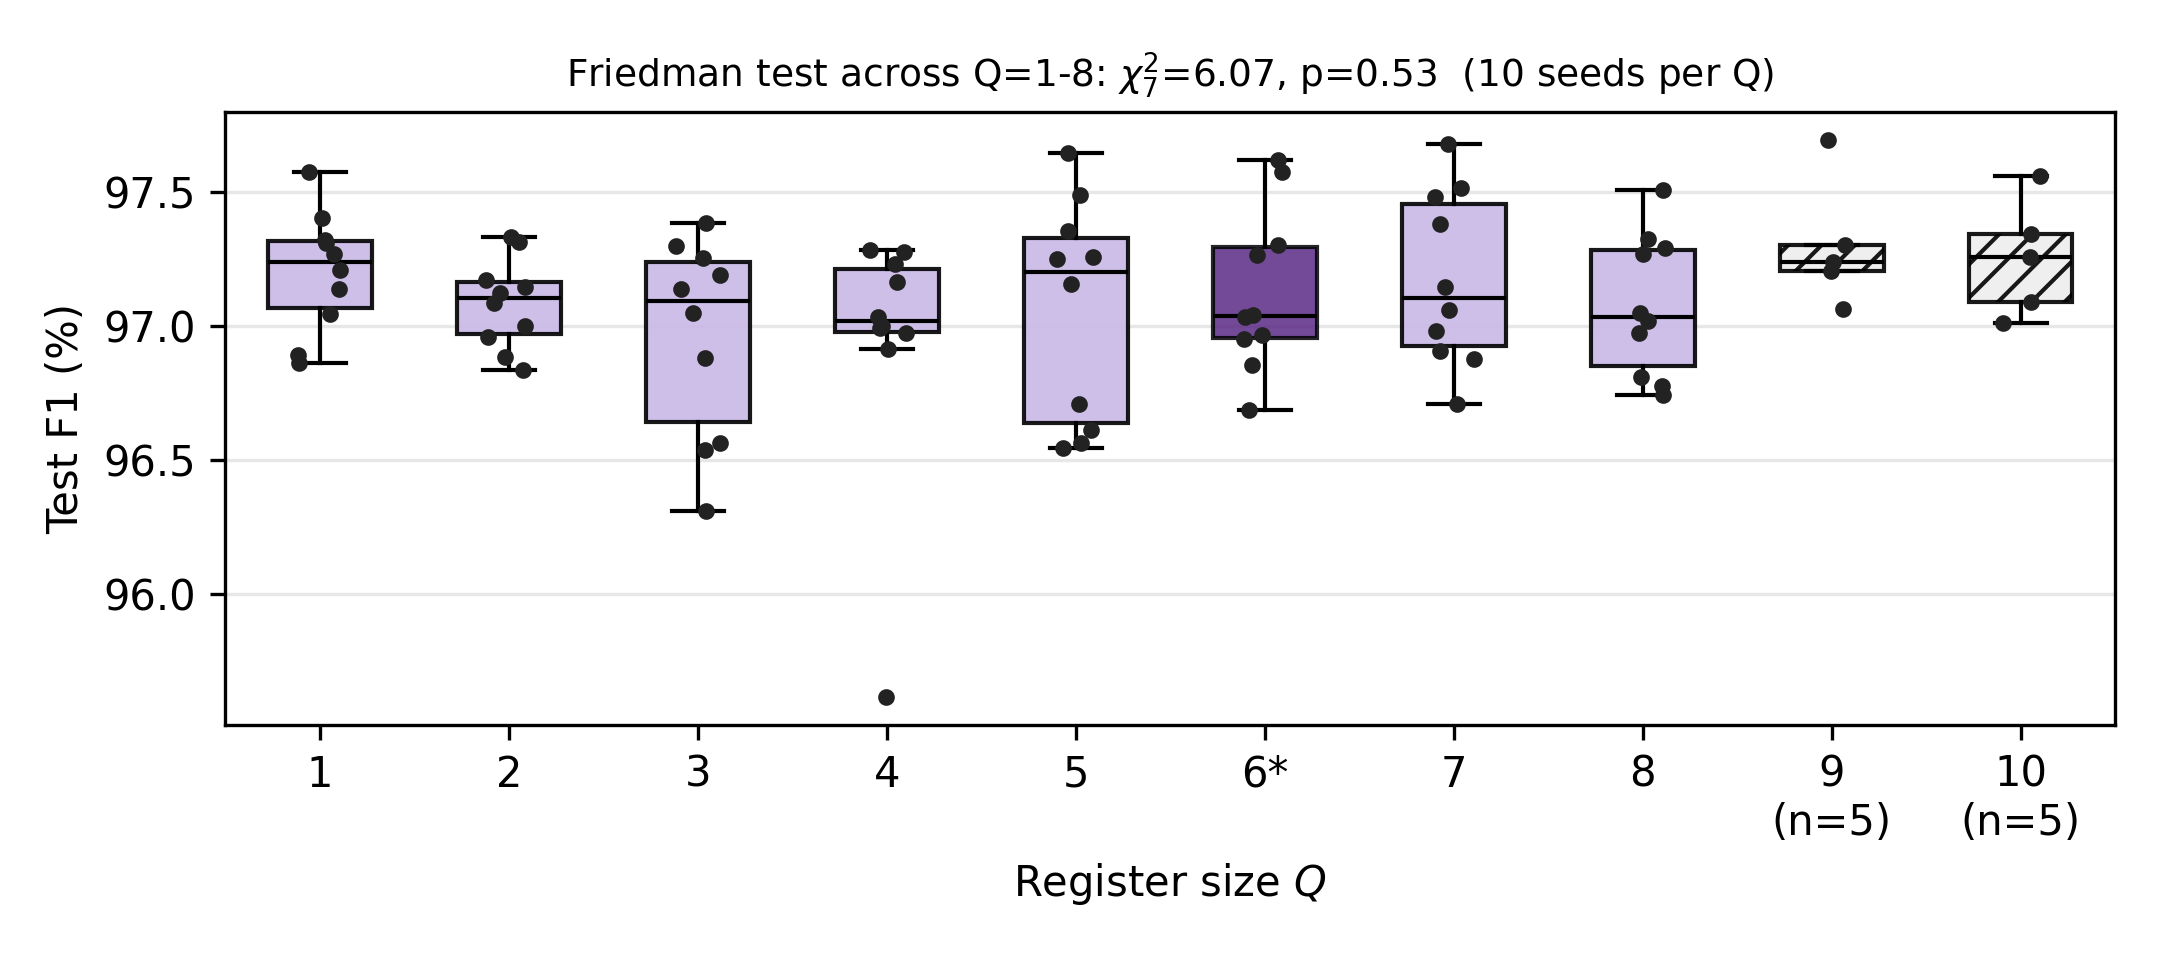
\includegraphics[width=\linewidth]{images/q_ablation_boxplot.png}
\caption{\textcolor{black}{Test F1 versus QPSO register size; hatched boxes use five seeds, the others ten.}}

\end{figure}

\textcolor{black}{\textbf{Search-budget sensitivity.}
Fig.~7(a) shows that the default budget does not fully
converge the search: a larger budget raises the best fitness found for
every $Q$, by 6--21\% at eight times the evaluations. For the trained
runs, the increase is significant, with Friedman $p<10^{-4}$ over the
four budgets and a gain of 387 from $20\times30$ to $40\times60$
(Wilcoxon $p<10^{-6}$). Intermediate $Q$ from 3 to 6 reaches the
highest fitness at every budget, consistent with
Fig.~3. The additional search, however, does not
improve detection, as Table~XIV and
Fig.~7(b) show. Test F1 stays within 96.9--97.3\% in every
cell, with no budget effect (Friedman $p=0.50$; $20\times30$ versus
$40\times60$: mean difference $-0.10$\,pp, Wilcoxon $p=0.15$), and
validation F1 even decreases slightly at $40\times60$ ($-0.6$\,pp,
$p=0.02$). Pushing the training-split fitness further thus mildly
overfits the selection. No degradation at $Q=7$ or 8 appears at any
budget, and the validation-selected $Q$ within 6 to 10 changes with
the budget, to 10, 7, 9, and 9, as expected when no setting is
genuinely better. Larger budgets therefore do not change the conclusion that detection is insensitive to $Q$.
Training detectors for all $Q$ from 1 to 10 at the largest budget of
$40\times60$ with five seeds confirms this: test F1 ranges from
96.89\% to 97.31\%, the Friedman test finds no effect of $Q$
($p=0.46$), and the validation-selected setting moves to $Q=9$. The
default budget of $20\times30$ is retained because it is sufficient
for detection at the lowest cost.}

\setcounter{figure}{6}
\begin{figure}[H]
\centering
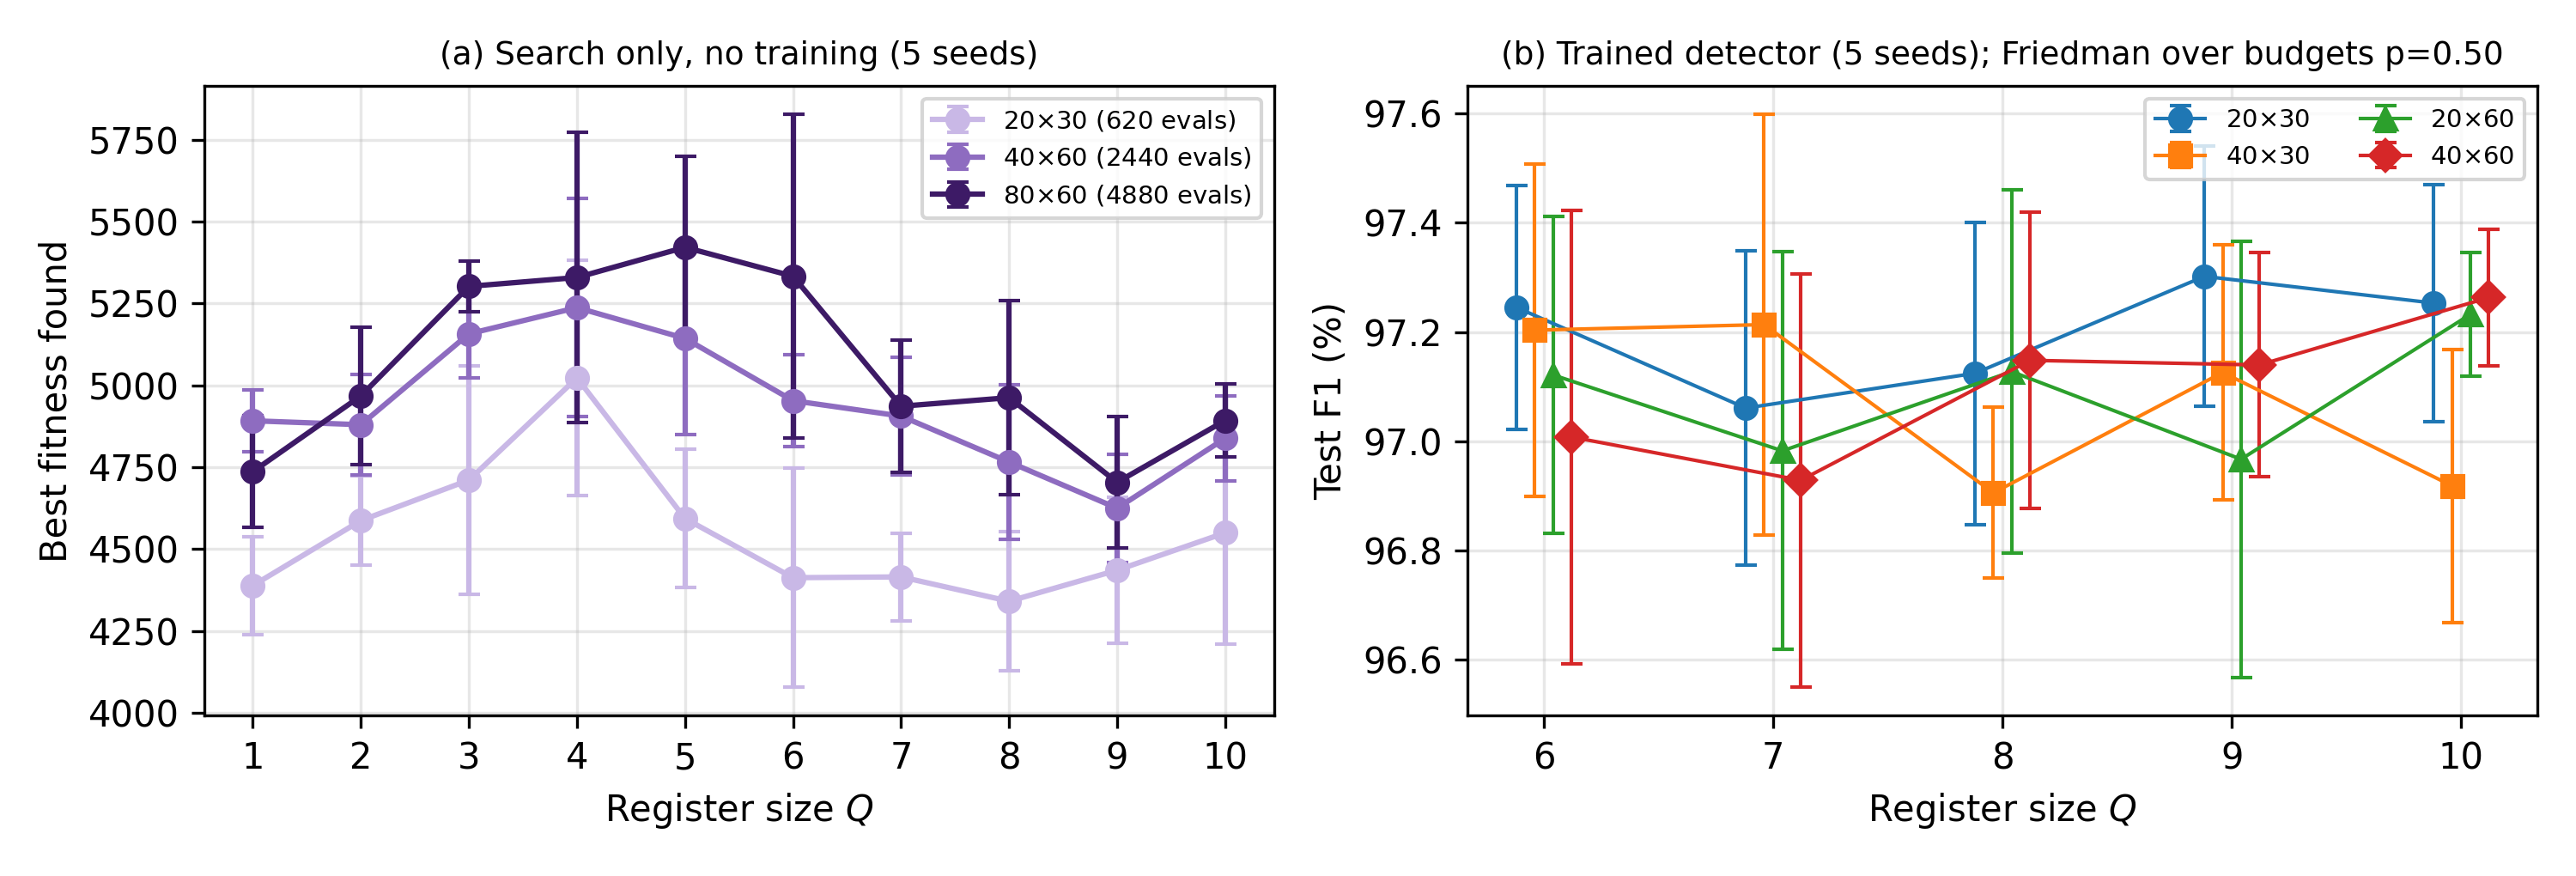
\includegraphics[width=0.9\linewidth]{images/budget_sensitivity.png}
\caption{\textcolor{black}{Search-budget sensitivity: (a)~best fitness of the search alone; (b)~test F1 of trained detectors.}}

\end{figure}

\setcounter{table}{13}
\begin{table}[H]
\centering
\scriptsize
\caption{\textcolor{black}{Search-budget sensitivity of QPSO over five seeds per cell.}}

\color{black}
\setlength{\tabcolsep}{3pt}
\begin{adjustbox}{max width=\linewidth}
\begin{tabular}{cccccc}
\hline\toprule
$Q$ & $P{\times}I$ & Evals & Fitness & Test F1 (\%) & Val.\ F1 (\%) \\
\hline\toprule
\multirow{4}{*}{6} & 20$\times$30 & 620 & 4412$\pm$334 & 97.25$\pm$0.22 & 96.10$\pm$1.08 \\
 & 40$\times$30 & 1240 & 4872$\pm$291 & 97.20$\pm$0.30 & 95.34$\pm$0.70 \\
 & 20$\times$60 & 1220 & 4856$\pm$317 & 97.12$\pm$0.29 & 94.73$\pm$0.89 \\
 & 40$\times$60 & 2440 & 4953$\pm$141 & 97.01$\pm$0.41 & 94.56$\pm$1.57 \\
\midrule
\multirow{4}{*}{7} & 20$\times$30 & 620 & 4415$\pm$134 & 97.06$\pm$0.29 & 95.74$\pm$1.13 \\
 & 40$\times$30 & 1240 & 4668$\pm$346 & 97.21$\pm$0.38 & 96.23$\pm$1.05 \\
 & 20$\times$60 & 1220 & 4886$\pm$248 & 96.98$\pm$0.36 & 95.72$\pm$1.26 \\
 & 40$\times$60 & 2440 & 4906$\pm$181 & 96.93$\pm$0.38 & 95.58$\pm$0.59 \\
\midrule
\multirow{4}{*}{8} & 20$\times$30 & 620 & 4340$\pm$212 & 97.12$\pm$0.28 & 96.13$\pm$0.48 \\
 & 40$\times$30 & 1240 & 4530$\pm$130 & 96.91$\pm$0.16 & 94.98$\pm$0.36 \\
 & 20$\times$60 & 1220 & 4749$\pm$360 & 97.13$\pm$0.33 & 95.64$\pm$0.52 \\
 & 40$\times$60 & 2440 & 4766$\pm$237 & 97.15$\pm$0.27 & 95.40$\pm$0.73 \\
\midrule
\multirow{4}{*}{9} & 20$\times$30 & 620 & 4435$\pm$222 & 97.30$\pm$0.24 & 95.89$\pm$0.89 \\
 & 40$\times$30 & 1240 & 4423$\pm$208 & 97.13$\pm$0.23 & 95.88$\pm$0.87 \\
 & 20$\times$60 & 1220 & 4473$\pm$399 & 96.97$\pm$0.40 & 95.98$\pm$0.49 \\
 & 40$\times$60 & 2440 & 4625$\pm$165 & 97.14$\pm$0.21 & 95.93$\pm$0.99 \\
\midrule
\multirow{4}{*}{10} & 20$\times$30 & 620 & 4550$\pm$341 & 97.25$\pm$0.22 & 96.18$\pm$0.90 \\
 & 40$\times$30 & 1240 & 4441$\pm$224 & 96.92$\pm$0.25 & 95.46$\pm$0.84 \\
 & 20$\times$60 & 1220 & 4664$\pm$285 & 97.23$\pm$0.11 & 95.80$\pm$1.36 \\
 & 40$\times$60 & 2440 & 4838$\pm$130 & 97.26$\pm$0.13 & 95.56$\pm$1.69 \\
\hline\toprule
\end{tabular}
\end{adjustbox}
\end{table}

\textcolor{red}{\textbf{Selected features and stability.}
Every mask contains exactly 40 of the 86 features, or 47\%, because $k$
is fixed for all selectors; QPSO determines which features are kept,
not how many. Fig.~8 shows how often each
feature is selected across seeds for every $Q$. A small core is
selected consistently: the context feature \texttt{syn\_frac\_src\_60}
appears in all 90 masks for $Q=1$ to 10 and \texttt{Protocol} in 92\%
of them, whereas \texttt{Src Port}, \texttt{Subflow Fwd Packets}, and
\texttt{dport\_switch} are never selected. Beyond this core, the masks
vary between seeds. At $Q^{*}=6$, the mean pairwise Jaccard index of
the selected sets is 0.36, against 0.30 for two random 40-feature
subsets, and it lies between 0.34 and 0.38 for every $Q$. Much of this
variation is substitution between redundant features: grouping
features whose absolute Spearman correlation on $\mathcal{D}_{\rm tr}$
is at least 0.9 gives 52 redundancy families, and at the family level
the Jaccard index rises to 0.53, against 0.45 for random subsets.
Seed-to-seed variation in the mask therefore does not translate into
variation in detection, which stays at $97.13\pm0.31\%$ F1 at
$Q^{*}=6$.}
\end{excerpt}
\begin{excerpt}
\setcounter{figure}{7}
\begin{figure}[H]
\centering

\includegraphics[width=\linewidth]{images/feature_selection_heatmap.png}
\caption{\textcolor{red}{Selection frequency of each feature for every register size; dots mark the consensus mask.}}

\end{figure}

\textcolor{red}{Table~XI lists the
deployed consensus mask at $Q^{*}=6$. Every feature in it is selected
in at least half of the ten runs, 8 of the 40 are context features,
and its trace-ratio fitness of 5089 exceeds that of the individual
runs, $4401\pm297$. Trained with ten seeds, the consensus mask reaches
$97.27\pm0.23\%$ F1 against $97.13\pm0.31\%$ for the individual masks
(Wilcoxon $p=0.38$), with 2.93\% missed attacks against 3.33\%
($p=0.18$). A single, seed-independent mask can therefore be deployed
without loss of detection. Because $k=40$ retains 47\% of the
features, this subset is not described as compact. A compact operating
point does exist: with $k=20$, or 23\% of the features, QPSO reaches
$96.51\pm0.67\%$ F1 over ten seeds, 0.62\,pp below $k=40$, whereas
$k=10$ drops to $93.82\pm1.05\%$. $k=40$ is kept as the default, and
$k=20$ is reported for deployments that require fewer features.}
\end{excerpt}

\loc{(c) Pages 4--5: Added the zero-variance filter to Section III-A}
\begin{excerpt}
\mshead{III-A}{Data Processing and Context-Aware Feature Representation}


Raw flow records $\mathbf{X}(t)$ are mapped by a seed-controlled,
deterministic preprocessing pipeline $\mathcal{P}$ to a unified
representation
\begin{equation}
\mathbf{X}(t) \xrightarrow{\mathcal{P}}
\mathbf{F}_s \oplus \mathbf{F}_c = \mathbf{Z},
\tag{3}
\end{equation}
where $\mathbf{F}_s$ denotes static flow descriptors and
$\mathbf{F}_c$ context-aware features.
\textcolor{black}{$\mathbf{F}_s$ contains the 75 CICFlowMeter
descriptors: ports, protocol, flow duration, packet and byte counts,
packet-length statistics, inter-arrival times, flag counts, and bulk
and activity statistics. Flow identifiers, IP addresses, and
timestamps are excluded to prevent identity shortcuts. The four
\texttt{Idle} fields are also excluded, because in ACI-IoT they store
absolute epoch timestamps and would leak capture time.}
$\mathbf{F}_c$ captures burst activity, dormant intervals, and
protocol state transitions that static descriptors alone do not
reveal. A single global seed controls the
\textcolor{black}{measurement} sampling in QPSO and the
weight initialization of the classifier.

\textcolor{black}{Table~IV defines
the 17 context features. Flows are sorted by timestamp, and ties at
the 1\,s resolution keep capture order, so ``earlier'' means a
position $j<i$ in the sorted stream. Let $s_i$, $t_i$, $\pi_i$,
$p_i$, and $a_i$ denote the source IP, timestamp, protocol,
destination port, and destination IP of flow $i$; the source IP
serves only as a grouping key, never as a feature. For a look-back
window $W$, the history of flow $i$ is}
\begin{equation}
\textcolor{black}{\mathcal{H}_W(i)=\{\,j<i:\ s_j=s_i,\ t_j\ge t_i-W\,\},}
\tag{4}
\end{equation}
\textcolor{black}{and $\mathrm{prev}(i)$ is the most recent
earlier flow of the same source. In Table~IV,
$n^{\rm pk}_j$ and $n^{\rm by}_j$ are the packets and bytes of flow
$j$ in both directions, and $\mathbf{1}[\cdot]$ is the indicator
function. Flow $i$ itself is excluded, so
every feature depends only on past traffic of the same source and
uses no labels. Two windows are used: $W=10$\,s for short scanning
and flooding bursts, and $W=60$\,s for slower propagation and
dormancy. Both were fixed before the experiments and not tuned.
Context features are computed on the full chronological stream
before subsampling, so window statistics reflect real traffic
density.}

\textcolor{black}{ACI-IoT stores most timestamps in
year--day--month order (e.g., \texttt{2023-01-11} denotes
1~November~2023) and part of the benign traffic in a day/month
12-hour format. Both formats are parsed accordingly, and the result
was verified against the epoch-microsecond values of the
\texttt{Idle} fields. A streaming implementation that keeps each
source's flows from the last 60\,s yields values identical to the
batch computation; its per-flow cost is reported in
Section~IV-B.}

\setcounter{table}{3}
\begin{table}[H]
\centering
\scriptsize
\caption{\textcolor{black}{Definitions of the 17 context
features. Default is the value used when the source has no earlier
flow.}}

\color{black}
\setlength{\tabcolsep}{6pt}
\renewcommand{\arraystretch}{1.25}
\begin{adjustbox}{max width=\linewidth}
\begin{tabular}{l l >{\raggedright\arraybackslash}p{4.3cm} c c c}
\hline\toprule
\textbf{Group} & \textbf{Feature} & \textbf{Definition} & \textbf{$W$ (s)} & \textbf{Default} & \textbf{Dim.} \\
\hline\toprule
\multirow{3}{*}{Burst}
 & \texttt{n\_flows\_src\_W}    & $|\mathcal{H}_W(i)|$ & 10, 60 & 0 & 2 \\
 & \texttt{pkt\_rate\_src\_W}   & $\sum_{j\in\mathcal{H}_W(i)} n^{\rm pk}_j \,/\, W$ & 10, 60 & 0 & 2 \\
 & \texttt{bytes\_rate\_src\_W} & $\sum_{j\in\mathcal{H}_W(i)} n^{\rm by}_j \,/\, W$ & 10, 60 & 0 & 2 \\
\midrule
\multirow{3}{*}{Dormant interval}
 & \texttt{dt\_prev\_src}     & $t_i-t_{\mathrm{prev}(i)}$ & -- & $10^{6}$ & 1 \\
 & \texttt{dt\_prev\_src\_log} & $\log(1+\texttt{dt\_prev\_src})$ & -- & $\log(1+10^{6})$ & 1 \\
 & \texttt{max\_gap\_src\_60}  & Max.\ gap between consecutive flows in $\mathcal{H}_{60}(i)\cup\{i\}$ & 60 & 60 & 1 \\
\midrule
\multirow{2}{*}{Diversity}
 & \texttt{n\_distinct\_dst\_W}   & $|\{a_j: j\in\mathcal{H}_W(i)\}|$ & 10, 60 & 0 & 2 \\
 & \texttt{n\_distinct\_dport\_W} & $|\{p_j: j\in\mathcal{H}_W(i)\}|$ & 10, 60 & 0 & 2 \\
\midrule
\multirow{4}{*}{Transition}
 & \texttt{proto\_switch}       & $\mathbf{1}[\pi_i\neq\pi_{\mathrm{prev}(i)}]$ & -- & 0 & 1 \\
 & \texttt{dport\_switch}       & $\mathbf{1}[p_i\neq p_{\mathrm{prev}(i)}]$ & -- & 0 & 1 \\
 & \texttt{n\_proto\_switch\_60} & $\sum_{j\in\mathcal{H}_{60}(i)} \texttt{proto\_switch}_j$ & 60 & 0 & 1 \\
 & \texttt{syn\_frac\_src\_60}  & Share of flows in $\mathcal{H}_{60}(i)$ with $\mathrm{SYN}_j>0$ & 60 & 0 & 1 \\
\midrule
\multicolumn{5}{l}{\textbf{Total} (burst 6, dormant interval 3, diversity 4, transition 4)} & \textbf{17} \\
\hline\toprule
\end{tabular}
\end{adjustbox}
\end{table}

\textcolor{red}{Six CICFlowMeter fields (\texttt{Bwd PSH Flags},
\texttt{Bwd URG Flags}, \texttt{Fwd Bytes/Bulk Avg},
\texttt{Fwd Packet/Bulk Avg}, \texttt{Fwd Bulk Rate Avg},
\texttt{Subflow Bwd Packets}) are constant on $\mathcal{D}_{\rm tr}$
and are removed by a zero-variance filter fitted on
$\mathcal{D}_{\rm tr}$ only. Without this filter, such columns could
be selected at no cost: they leave both sums of the trace-ratio
fitness in Eq.~(12) unchanged and only occupy mask slots.}
\textcolor{black}{\textcolor{red}{The fused representation therefore has
$d=86$ features (69 static and 17 context).}}
\end{excerpt}

%% ---------------------------------------------------------------------
\review{1.5}{In Section III-B and III-E, manuscript p.~6, the QPSO fitness repeatedly evaluates candidate masks using F1, AUC, MSE, and error-balance terms. The manuscript should explicitly state which data split is used for each selection step and confirm that the test set is never used for QPSO fitness, Q selection, weight tuning, or early stopping.}

\reply We thank the reviewer for this essential comment. The revised
manuscript states the split used by every step and confirms that the test
set is used only for reporting. The QPSO fitness is now the Fisher trace
ratio of the selected features (Eq.~(12)), a label-based filter criterion
computed on the training split only; it contains no F1, AUC, MSE, or
error-balance terms and therefore has no weights to tune. $Q^{*}$ is
selected on the validation split, early stopping and the learning-rate
schedule monitor the validation loss, the zero-variance filter and the
min--max normalization are fitted on the training split, and the search
budget, $k$, and the classifier hyperparameters were fixed before the
experiments. The data split itself is now a blocked temporal split with a
purge gap, so no window spans two splits. Table~VII lists the data used by
every fitting, selection, and stopping step.

\loc{(a) Pages 5--6: Added the leakage-free blocked temporal split to Section III-A}
\begin{excerpt}
\mshead{III-A}{Data Processing and Context-Aware Feature Representation}


Raw flow records $\mathbf{X}(t)$ are mapped by a seed-controlled,
deterministic preprocessing pipeline $\mathcal{P}$ to a unified
representation
\begin{equation}
\mathbf{X}(t) \xrightarrow{\mathcal{P}}
\mathbf{F}_s \oplus \mathbf{F}_c = \mathbf{Z},
\tag{3}
\end{equation}
where $\mathbf{F}_s$ denotes static flow descriptors and
$\mathbf{F}_c$ context-aware features.
\textcolor{black}{$\mathbf{F}_s$ contains the 75 CICFlowMeter
descriptors: ports, protocol, flow duration, packet and byte counts,
packet-length statistics, inter-arrival times, flag counts, and bulk
and activity statistics. Flow identifiers, IP addresses, and
timestamps are excluded to prevent identity shortcuts. The four
\texttt{Idle} fields are also excluded, because in ACI-IoT they store
absolute epoch timestamps and would leak capture time.}
$\mathbf{F}_c$ captures burst activity, dormant intervals, and
protocol state transitions that static descriptors alone do not
reveal. A single global seed controls the
\textcolor{black}{measurement} sampling in QPSO and the
weight initialization of the classifier.

\textcolor{black}{Table~IV defines
the 17 context features. Flows are sorted by timestamp, and ties at
the 1\,s resolution keep capture order, so ``earlier'' means a
position $j<i$ in the sorted stream. Let $s_i$, $t_i$, $\pi_i$,
$p_i$, and $a_i$ denote the source IP, timestamp, protocol,
destination port, and destination IP of flow $i$; the source IP
serves only as a grouping key, never as a feature. For a look-back
window $W$, the history of flow $i$ is}
\begin{equation}
\textcolor{black}{\mathcal{H}_W(i)=\{\,j<i:\ s_j=s_i,\ t_j\ge t_i-W\,\},}
\tag{4}
\end{equation}
\textcolor{black}{and $\mathrm{prev}(i)$ is the most recent
earlier flow of the same source. In Table~IV,
$n^{\rm pk}_j$ and $n^{\rm by}_j$ are the packets and bytes of flow
$j$ in both directions, and $\mathbf{1}[\cdot]$ is the indicator
function. Flow $i$ itself is excluded, so
every feature depends only on past traffic of the same source and
uses no labels. Two windows are used: $W=10$\,s for short scanning
and flooding bursts, and $W=60$\,s for slower propagation and
dormancy. Both were fixed before the experiments and not tuned.
Context features are computed on the full chronological stream
before subsampling, so window statistics reflect real traffic
density.}

\textcolor{black}{ACI-IoT stores most timestamps in
year--day--month order (e.g., \texttt{2023-01-11} denotes
1~November~2023) and part of the benign traffic in a day/month
12-hour format. Both formats are parsed accordingly, and the result
was verified against the epoch-microsecond values of the
\texttt{Idle} fields. A streaming implementation that keeps each
source's flows from the last 60\,s yields values identical to the
batch computation; its per-flow cost is reported in
Section~IV-B.}

\setcounter{table}{3}
\begin{table}[H]
\centering
\scriptsize
\caption{\textcolor{black}{Definitions of the 17 context
features. Default is the value used when the source has no earlier
flow.}}

\color{black}
\setlength{\tabcolsep}{6pt}
\renewcommand{\arraystretch}{1.25}
\begin{adjustbox}{max width=\linewidth}
\begin{tabular}{l l >{\raggedright\arraybackslash}p{4.3cm} c c c}
\hline\toprule
\textbf{Group} & \textbf{Feature} & \textbf{Definition} & \textbf{$W$ (s)} & \textbf{Default} & \textbf{Dim.} \\
\hline\toprule
\multirow{3}{*}{Burst}
 & \texttt{n\_flows\_src\_W}    & $|\mathcal{H}_W(i)|$ & 10, 60 & 0 & 2 \\
 & \texttt{pkt\_rate\_src\_W}   & $\sum_{j\in\mathcal{H}_W(i)} n^{\rm pk}_j \,/\, W$ & 10, 60 & 0 & 2 \\
 & \texttt{bytes\_rate\_src\_W} & $\sum_{j\in\mathcal{H}_W(i)} n^{\rm by}_j \,/\, W$ & 10, 60 & 0 & 2 \\
\midrule
\multirow{3}{*}{Dormant interval}
 & \texttt{dt\_prev\_src}     & $t_i-t_{\mathrm{prev}(i)}$ & -- & $10^{6}$ & 1 \\
 & \texttt{dt\_prev\_src\_log} & $\log(1+\texttt{dt\_prev\_src})$ & -- & $\log(1+10^{6})$ & 1 \\
 & \texttt{max\_gap\_src\_60}  & Max.\ gap between consecutive flows in $\mathcal{H}_{60}(i)\cup\{i\}$ & 60 & 60 & 1 \\
\midrule
\multirow{2}{*}{Diversity}
 & \texttt{n\_distinct\_dst\_W}   & $|\{a_j: j\in\mathcal{H}_W(i)\}|$ & 10, 60 & 0 & 2 \\
 & \texttt{n\_distinct\_dport\_W} & $|\{p_j: j\in\mathcal{H}_W(i)\}|$ & 10, 60 & 0 & 2 \\
\midrule
\multirow{4}{*}{Transition}
 & \texttt{proto\_switch}       & $\mathbf{1}[\pi_i\neq\pi_{\mathrm{prev}(i)}]$ & -- & 0 & 1 \\
 & \texttt{dport\_switch}       & $\mathbf{1}[p_i\neq p_{\mathrm{prev}(i)}]$ & -- & 0 & 1 \\
 & \texttt{n\_proto\_switch\_60} & $\sum_{j\in\mathcal{H}_{60}(i)} \texttt{proto\_switch}_j$ & 60 & 0 & 1 \\
 & \texttt{syn\_frac\_src\_60}  & Share of flows in $\mathcal{H}_{60}(i)$ with $\mathrm{SYN}_j>0$ & 60 & 0 & 1 \\
\midrule
\multicolumn{5}{l}{\textbf{Total} (burst 6, dormant interval 3, diversity 4, transition 4)} & \textbf{17} \\
\hline\toprule
\end{tabular}
\end{adjustbox}
\end{table}

\textcolor{black}{Six CICFlowMeter fields (\texttt{Bwd PSH Flags},
\texttt{Bwd URG Flags}, \texttt{Fwd Bytes/Bulk Avg},
\texttt{Fwd Packet/Bulk Avg}, \texttt{Fwd Bulk Rate Avg},
\texttt{Subflow Bwd Packets}) are constant on $\mathcal{D}_{\rm tr}$
and are removed by a zero-variance filter fitted on
$\mathcal{D}_{\rm tr}$ only. Without this filter, such columns could
be selected at no cost: they leave both sums of the trace-ratio
fitness in Eq.~(12) unchanged and only occupy mask slots.}
\textcolor{red}{The fused representation therefore has
$d=86$ features (69 static and 17 context).}

\textcolor{red}{A class-balanced subsample of 80{,}000
flows (40{,}000 benign and 40{,}000 attack, with attack-type
proportions preserved) is drawn with a fixed seed and re-sorted
chronologically. ACI-IoT attacks are clustered in time, so a purely
chronological 70/15/15 split would leave $\mathcal{D}_{\rm te}$
entirely benign. We therefore use a blocked temporal split. The
stream is cut into contiguous 500-flow blocks, which a seeded shuffle
assigns to $\mathcal{D}_{\rm tr}$, $\mathcal{D}_{\rm va}$, and
$\mathcal{D}_{\rm te}$ (70/15/15), and the first $T=10$ flows of
every block are purged. Sliding windows of length $T=10$ are built
only within a block, so no window spans two splits. The splits
contain 54{,}890 / 11{,}760 / 11{,}760 flows with attack fractions
of 47.5\% / 53.6\% / 58.2\%; $\mathcal{D}_{\rm tr}$ covers all ten
attack types, $\mathcal{D}_{\rm va}$ seven, and $\mathcal{D}_{\rm te}$
six.}
\end{excerpt}
\begin{excerpt}
The fused representation is normalized as
\begin{equation}
\mathbf{Z}_n = \mathcal{N}(\mathbf{Z}),\quad
\mathbf{Z}_n \in [0,1]^d.
\tag{5}
\end{equation}
\textcolor{red}{The min--max parameters are computed on
$\mathcal{D}_{\rm tr}$ only and applied unchanged to
$\mathcal{D}_{\rm va}$ and $\mathcal{D}_{\rm te}$, with values
outside $[0,1]$ clipped.}
\end{excerpt}

\loc{(b) Pages 7--9: Added the data used by each fitting, selection, and stopping step to Section III-B}
\begin{excerpt}
\mshead{III-B}{Variable-Qubit QPSO Feature Selection}


QPSO learns a sparse binary feature mask
$\mathbf{m}\in\{0,1\}^d$ that gates the normalized input:
\begin{equation}
\tilde{\mathbf{z}} = \mathbf{m}\odot\mathbf{z}_n,\quad
\|\mathbf{m}\|_0 = k \ll d,
\tag{6}
\end{equation}
where $\odot$ denotes element-wise multiplication.
\textcolor{black}{Each of the $P$ particles $i$ holds a
non-negative amplitude vector $\mathbf{a}_i\in\mathbb{R}_{\ge 0}^{d}$
with $\sum_j a_{i,j}=1$, one amplitude per feature, so the particle
dimension is $d$ for every $Q$. The register size $Q$ enters the
search at three points. First, amplitudes are initialized at the
uniform amplitude of a $Q$-qubit register plus Gaussian noise; after
normalization, only the relative perturbation
$\rho(Q)=2^{Q/2}/(Q^{2}+1)$ matters:}
\begin{equation}
\textcolor{black}{a_{i,j}^{(0)} \propto \Bigl|\,2^{-Q/2} +
\tfrac{\xi_{i,j}}{Q^{2}+1}\Bigr|,\quad
\xi_{i,j}\sim\mathcal{N}(0,1).}
\tag{7}
\end{equation}
\textcolor{black}{Second, at iteration $t$, each particle is
rotated toward its personal-best amplitude $\mathbf{a}_i^{\rm pb}$
and the global-best amplitude $\mathbf{a}^{\rm gb}$ by an angle whose
upper bound decreases with $Q$:}
\begin{align}
\textcolor{black}{\phi_t} &\textcolor{black}{= \frac{\pi}{2Q}\Bigl(1-\frac{t}{I}\Bigr),}
\tag{8}\\
\textcolor{black}{\mathbf{a}_i} &\textcolor{black}{\leftarrow \mathbf{a}_i
+ r_1\cos\phi_t\,(\mathbf{a}_i^{\rm pb}-\mathbf{a}_i)
+ r_2\sin\phi_t\,(\mathbf{a}^{\rm gb}-\mathbf{a}_i),}
\tag{9}
\end{align}
\textcolor{black}{with $r_1,r_2\sim\mathcal{U}(0,1)$ drawn per
particle and iteration. Third, each amplitude independently
``collapses'' to a fresh random value with a probability that decays
exponentially in $Q$, and the vector is then renormalized:}
\begin{equation}
\textcolor{black}{a_{i,j} \leftarrow u_{i,j}\sim\mathcal{U}(0,1)
\ \text{w.p. } 2^{-Q},\quad
\mathbf{a}_i \leftarrow |\mathbf{a}_i| / \|\mathbf{a}_i\|_1 .}
\tag{10}
\end{equation}
\textcolor{black}{A mask is obtained by measurement: $k$
distinct feature indices are drawn without replacement with
probabilities $\pi_{i,j}=a_{i,j}^{2}/\sum_{l}a_{i,l}^{2}$, and
$m_{i,j}=1$ for the drawn indices,}
\begin{equation}
\textcolor{black}{\mathbf{m}_i = \textsc{Measure}_k(\boldsymbol{\pi}_i),
\qquad \|\mathbf{m}_i\|_0 = k .}
\tag{11}
\end{equation}
\textcolor{black}{Each run returns $\mathbf{m}^{*}$, the
highest-fitness mask measured during the search, as in standard PSO.
Hence $k$ is a fixed design parameter, set to 40 in all experiments,
and $Q$ shapes \emph{which} $k$ features are found, not how many.
Algorithm~1 summarizes the procedure, and
Table~V lists the constants set by each $Q$.}
\textcolor{black}{Because a single run's mask depends on its
seed, the deployed detector uses a consensus mask
$\mathbf{m}^{*}_{\rm cons}$: the $k$ features selected most often
across the ten QPSO runs at the selected $Q^{*}$, with ties broken by
the summed fitness of the runs that selected them. All ten runs use
$\mathcal{D}_{\rm tr}$ only, so the consensus uses no validation or
test data.}

\setcounter{table}{4}
\begin{table}[H]
\centering
\scriptsize
\caption{\textcolor{black}{Search constants set by the
register size for the 86 input features.}}

\setlength{\tabcolsep}{4pt}
\renewcommand{\arraystretch}{1.05}
\color{black}
\begin{adjustbox}{max width=\linewidth}
\begin{tabular}{cccccc}
\hline\toprule
$Q$ & \makecell{Initial\\perturb.} & \makecell{Max.\ rot.\\(deg)} & \makecell{Reset\\prob.} & \makecell{Resets per\\particle-iter.} & Regime \\
\hline\toprule
1  & 0.71 & 90.0 & 0.500  & 43.0 & near-random \\
2  & 0.40 & 45.0 & 0.250  & 21.5 & exploratory \\
3  & 0.28 & 30.0 & 0.125  & 10.8 & exploratory \\
4  & 0.24 & 22.5 & 0.063  & 5.38 & balanced \\
5  & 0.22 & 18.0 & 0.031  & 2.69 & balanced \\
6  & 0.22 & 15.0 & 0.016  & 1.34 & balanced \\
7  & 0.23 & 12.9 & 0.008  & 0.67 & exploitative \\
8  & 0.25 & 11.3 & 0.004  & 0.34 & exploitative \\
9  & 0.29 & 10.0 & 0.002  & 0.17 & near-frozen \\
10 & 0.32 & 9.0  & 0.001  & 0.08 & near-frozen \\
\hline\toprule
\end{tabular}
\end{adjustbox}
\end{table}

\setcounter{algorithm}{0}
\begin{algorithm}[H]
\caption{\textcolor{black}{Variable-qubit QPSO feature
selection. Steps commented with Q are the only ones that depend on
the register size.}}

\color{black}
\small
\begin{algorithmic}[1]
\Require $\mathbf{Z}_{\rm tr}\in[0,1]^{N\times d}$, labels $\mathbf{y}_{\rm tr}$, register size $Q$, particles $P$, iterations $I$, subset size $k$
\Ensure Mask $\mathbf{m}^{*}\in\{0,1\}^{d}$ with $\|\mathbf{m}^{*}\|_0=k$
\For{$i=1$ to $P$}
  \State $\mathbf{a}_i\gets$ Eq.~(7), normalized \Comment{$Q$}
  \State $\mathbf{m}_i\gets\textsc{Measure}_k(\mathbf{a}_i)$; $J_i\gets\mathcal{J}(\mathbf{m}_i)$ on $\mathcal{D}_{\rm tr}$
  \State $\mathbf{a}_i^{\rm pb}\gets\mathbf{a}_i$; $J_i^{\rm pb}\gets J_i$
\EndFor
\State $i^{\star}\gets\arg\max_i J_i$; $\mathbf{a}^{\rm gb}\gets\mathbf{a}_{i^{\star}}$; $\mathbf{m}^{*}\gets\mathbf{m}_{i^{\star}}$; $J^{*}\gets J_{i^{\star}}$
\For{$t=0$ to $I-1$}
  \State $\phi_t\gets\frac{\pi}{2Q}(1-t/I)$ \Comment{$Q$}
  \For{$i=1$ to $P$}
    \State $\mathbf{a}_i\gets$ rotation toward $\mathbf{a}_i^{\rm pb},\mathbf{a}^{\rm gb}$, Eq.~(9)
    \State reset each $a_{i,j}$ w.p.\ $2^{-Q}$; normalize, Eq.~(10) \Comment{$Q$}
    \State $\mathbf{m}_i\gets\textsc{Measure}_k(\mathbf{a}_i)$, Eq.~(11); $J_i\gets\mathcal{J}(\mathbf{m}_i)$
    \If{$J_i>J_i^{\rm pb}$}
      \State $\mathbf{a}_i^{\rm pb}\gets\mathbf{a}_i$; $J_i^{\rm pb}\gets J_i$
    \EndIf
    \If{$J_i>J^{*}$}
      \State $\mathbf{a}^{\rm gb}\gets\mathbf{a}_i$; $\mathbf{m}^{*}\gets\mathbf{m}_i$; $J^{*}\gets J_i$
    \EndIf
  \EndFor
\EndFor
\State \Return $\mathbf{m}^{*}$ \Comment{$P(I+1)$ fitness evaluations}
\end{algorithmic}
\end{algorithm}

\textcolor{black}{Table~V shows
how $Q$ shapes the search. With a single qubit, the rotation bound is
$\pi/2$ and half of all amplitudes are reset at every iteration, so
the search is close to random sampling. As $Q$ grows, the bound
shrinks, the personal-best term dominates the update, and from $Q=7$
onward fewer than one amplitude per particle is reset at each
iteration. $Q$ therefore
moves the search from exploration to exploitation, with a risk of
premature convergence at large $Q$ under a finite budget. Beyond
$Q=8$, resets are rare and the pull toward the global best is weak,
so the search stays close to its initialization. The trained-detector
ablation therefore covers $Q=1$ to $8$, and the budget analysis
extends the range to $Q=10$ to confirm this behavior.}

\textcolor{black}{CONQUEST is quantum-\emph{inspired} and runs
on classical hardware: no $2^{Q}$-dimensional state vector is
simulated, and the particle dimension is $d$ for every $Q$. The term
``qubit'' refers to the register whose uniform amplitude $2^{-Q/2}$
and collapse probability $2^{-Q}$ motivate the three constants
above. $Q$ is thus a single interpretable hyperparameter that sets
the exploration schedule of the swarm, not a measure of model
capacity.}

\textcolor{black}{Fig.~3 confirms this
behavior empirically. Algorithm~1 is run on
$\mathcal{D}_{\rm tr}$ for $Q=1$ to $10$ with ten seeds, without
classifier training, and three regimes appear. At $Q=1$, the
amplitude entropy falls only to 0.75, because half of the amplitudes
are reset at every iteration, and the swarm keeps sampling almost
uniformly. For $Q=4$ to $7$, the entropy falls to 0.25--0.35 within a
few iterations and swarm diversity drops: the search concentrates on
a feature subset. For $Q\ge 9$, the entropy stays at 0.54--0.66,
because small rotations and rare resets barely move the particles.
The best fitness peaks at $Q=4$ and is lower at both extremes,
although the differences are within the seed-to-seed spread.
Returning the best evaluated mask matters most at large $Q$: a fresh
measurement of the final global-best amplitude retains 91\% of the
best fitness at $Q=1$ but only 44--52\% at $Q\ge9$, because those
amplitudes remain spread out and rarely reproduce the best subset.}

\setcounter{figure}{2}
\begin{figure}[H]
\centering

\includegraphics[width=0.95\linewidth]{images/qpso_dynamics_vs_Q.png}
\caption{\textcolor{black}{QPSO search dynamics versus register size over ten seeds: measurement entropy (left), mask diversity (middle), and best fitness (right).}}

\end{figure}

\textcolor{red}{Each measured mask is scored by the
Fisher trace ratio of its selected features, a class-separability
criterion referred to below as the trace-ratio fitness,}
\begin{equation}
\textcolor{red}{\mathcal{J}(\mathbf{m}) =
\frac{\sum_{c}n_c\,\|\boldsymbol{\mu}_c^{\mathbf{m}}-
\boldsymbol{\mu}^{\mathbf{m}}\|_2^{2}}
{\sum_{c}\sum_{j:m_j=1}\mathrm{Var}_c(z_j)+\epsilon},}
\tag{12}
\end{equation}
\textcolor{black}{where $c\in\{\text{benign},\text{attack}\}$, $n_c$
and $\boldsymbol{\mu}_c^{\mathbf{m}}$ are the class count and class
mean of the selected features, $\boldsymbol{\mu}^{\mathbf{m}}$ is
their overall mean, and $\epsilon=10^{-10}$. Personal and global
bests are updated when $\mathcal{J}$ improves. $\mathcal{J}$ is a
filter criterion that needs no classifier training, so one run with
20 particles and 30 iterations costs 620 fitness evaluations.}
\textcolor{black}{One run takes a median of 1.8\,min on the
host of Table~VI, and 5.0\,min at the largest
trained budget of 40 particles and 60 iterations.}

\setcounter{table}{5}
\begin{table}[H]
\centering
\caption{Experimental environment and implementation settings.}

\def\rc#1{\textcolor{red}{#1}}
\setlength{\tabcolsep}{8pt}
\renewcommand{\arraystretch}{1.3}
\begin{adjustbox}{max width=\linewidth}
\begin{tabular}{l l l l}
\hline\toprule
\textbf{Block} & \textbf{Item} & \textbf{Setting} & \textbf{Scope} \\
\hline\toprule
Environment & Platform & Windows 10, CPU only & All runs \\
 & Framework & TensorFlow 2.20.0, Python 3.13.5 & Training and inference \\
 & Determinism & \texttt{TF\_DETERMINISTIC\_OPS=1} & Seed-controlled \\
\midrule
Data & \rc{Subsample} & \rc{80k flows, class-balanced} & \rc{Fixed seed 42} \\
 & \rc{Split} & \rc{Blocked temporal, 70/15/15} & \rc{500-flow blocks} \\
 & Window length & $T=10$ flows & All regimes \\
 & \rc{Batch size} & \rc{32 centralized, 64 federated} & \rc{All regimes} \\
\midrule
Training & \rc{Optimizer} & \rc{SGD, Nesterov momentum 0.9} & \rc{Centralized and federated} \\
 & Learning rate & $10^{-3}$ & Centralized and federated \\
 & \rc{Stopping} & \rc{At most 35 epochs, patience 6} & \rc{Validation loss} \\
 & \rc{KL weight} & \rc{$\gamma=10^{-3}$} & \\
\midrule
Model & \rc{Encoder} & \rc{LSTM 256, 2-head attention, LSTM 128} & \rc{Dropout 0.2} \\
 & \rc{Latent size} & \rc{64} & \rc{LSTM(+VAE) variants} \\
\midrule
QPSO & Particles, iterations & $P=20$, $I=30$ & Default budget \\
 & \rc{Budget sensitivity} & \rc{$P=20$ or 40, $I=30$ or 60} & \rc{Five seeds} \\
 & \rc{Selected features} & \rc{$k=40$, fitness on $\mathcal{D}_{\rm tr}$} & \rc{All selectors} \\
 & \rc{Register size} & \rc{$Q=1$ to 8; $Q=9$, 10} & \rc{Ten seeds; five seeds} \\
\midrule
Federated & \rc{Clients} & \rc{$K=5$; 10 and 20 for sensitivity} & \rc{Full participation} \\
 & \rc{Rounds, local epochs} & \rc{$R=30$, $E=2$} & \rc{All FL experiments} \\
 & \rc{Mask construction} & \rc{Proxy (default), vote, central} & \rc{Shared by all clients} \\
 & Aggregators & FedAvg, SCAFFOLD, FLAME & Same partitions \\
\hline\toprule
\end{tabular}
\end{adjustbox}
\end{table}

\textcolor{red}{Table~VII lists the data
used by every step that fits, selects, or stops. The
QPSO fitness in Eq.~(12) is a label-based filter criterion
evaluated on $\mathcal{D}_{\rm tr}$ only; it contains no F1, AUC,
MSE, or error-balance terms and therefore has no weights to tune.
$Q^{*}$ is chosen on $\mathcal{D}_{\rm va}$, and early stopping and
the learning-rate schedule monitor the $\mathcal{D}_{\rm va}$ loss.
The search budget, $k=40$, and the classifier hyperparameters were
fixed before the experiments. $\mathcal{D}_{\rm te}$ is evaluated
once per trained model, after training, to report the final
metrics. In federated training, the global F1 on $\mathcal{D}_{\rm te}$
is also logged after every round to measure convergence, but it never
selects a round, a model, or a setting.}
\end{excerpt}
\setcounter{table}{6}
\begin{table}[H]
\centering
\scriptsize
\caption{\textcolor{red}{Data used by each fitting,
selection, and stopping step. The test set is used only for
reporting.}}

\color{red}
\setlength{\tabcolsep}{3pt}
\renewcommand{\arraystretch}{1.05}
\begin{adjustbox}{max width=\linewidth}
\begin{tabular}{p{2.6cm} p{3.6cm} c}
\hline\toprule
\textbf{Step} & \textbf{Data used} & \textbf{Test set?} \\
\hline\toprule
Zero-variance filter & $\mathcal{D}_{\rm tr}$ (features only) & no \\
Context features & Earlier flows of the same source, unlabelled & no \\
Min--max normalization & $\mathcal{D}_{\rm tr}$ (features only) & no \\
QPSO / PSO fitness & $\mathcal{D}_{\rm tr}$ & no \\
Variance selection (OS-CIDS) & $\mathcal{D}_{\rm tr}$ (features only) & no \\
Consensus mask & Ten masks fitted on $\mathcal{D}_{\rm tr}$ & no \\
Selection of $Q^{*}$ & $\mathcal{D}_{\rm va}$, mean F1 over seeds & no \\
Early stopping, LR schedule & $\mathcal{D}_{\rm va}$ loss & no \\
Budget, $k$, hyperparameters & Fixed a priori & no \\
Decision rule & Fixed $\arg\max$ & no \\
FL masks (proxy/vote/central) & Proxy slice / client partitions / all of $\mathcal{D}_{\rm tr}$ & no \\
FL stopping & Fixed $R=30$ rounds & no \\
\midrule
Reported metrics & $\mathcal{D}_{\rm te}$, once per trained model & yes \\
FL per-client metrics & Client-matched windows of $\mathcal{D}_{\rm te}$, final model only & yes \\
FL convergence ($R_{99}$) & Per-round global F1 on $\mathcal{D}_{\rm te}$, reporting only & yes \\
\hline\toprule
\end{tabular}
\end{adjustbox}
\end{table}

%% ---------------------------------------------------------------------
\review{1.6}{In Section III-E and Section IV-A, manuscript pp.~6 and 8--9, the +2.21 pp F1 improvement of QCIDS over OS-CIDS cannot be attributed specifically to QPSO because QCIDS changes both context-aware representation and feature selection. A proper ablation should isolate these two components.}

\reply We agree and have added the requested ablation. A $2\times2$ factorial
design crosses context features (off, on) with the selector (variance
ranking, QPSO), all with the same classifier, data protocol, and $k=40$, over
ten seeds (Table~X); a classical PSO selector at an equal search budget is
added as a further control. The ablation shows that neither component helps
on its own: context features lower the F1 of variance ranking by 0.51\,pp,
and QPSO on static features alone lowers F1 by 1.07\,pp. Combined, they raise
F1 by 1.23\,pp over QPSO alone and by 0.68\,pp over variance ranking with
context, and their interaction, $+1.74$\,pp ($p=0.002$), is the dominant
effect. The gain therefore comes from combining context features with
label-aware selection, not from QPSO alone. Under the leakage-free protocol,
CONQUEST has the highest mean F1, 97.13\%, but its F1 is not significantly
higher than that of OS-CIDS ($p=0.32$); the +2.21\,pp gain of the previous
version does not hold. The pipelines differ instead in the type of error:
CONQUEST misses significantly fewer attacks than OS-CIDS (3.33\% versus
4.21\%, $p=0.004$) at the cost of more false alarms (2.24\% versus 1.43\%).
The abstract, contributions, and conclusion have been revised to state this
result accurately.

\loc{(a) Page 9: Added the factorial design and the classical PSO control to Section III-E}
\begin{excerpt}
\mshead{III-E}{Centralized Training and Evaluation Protocol}


Centralized training establishes the upper-bound detection
performance under full data visibility. 
Two configurations are trained with the same optimizer and stopping
rule: OS-CIDS, a static IDS with variance-based feature selection,
and QCIDS, which adds context-aware features and QPSO feature
selection. \textcolor{red}{S-CIDS, the baseline of the conference
version~{[9]}, is quoted from that work for reference
only, because it was evaluated under a different protocol.}
OS-CIDS and QCIDS therefore differ in two factors at once.
\textcolor{red}{To separate them, a $2\times2$ factorial
ablation crosses context features (off, on) with the selector
(variance, QPSO), all with $k=40$ and the same classifier, so that the
effect of each factor and their interaction can be estimated. A
classical binary PSO selector provides a controlled comparison of
quantum-inspired and classical updates. It uses inertia 0.7,
acceleration coefficients $c_1=c_2=1.5$, a sigmoid position mapping,
top-$k$ decoding, the same trace-ratio fitness of Eq.~(12), and the
same budget of 620 fitness evaluations.}
\end{excerpt}

\loc{(b) Pages 12--13: Revised the overall comparison and added the factorial ablation to Section IV-A}
\begin{excerpt}
\mshead{IV-A}{Centralized Cyberworm Detection Performance}


Table~IX reports centralized detection
performance \textcolor{red}{of five pipelines that share the
classifier, the data protocol, and $k=40$. They differ only in the
feature representation, static only or static plus context, and in
the selector: variance ranking, classical PSO, or QPSO. They are named
OS-CIDS (variance ranking, static only), Var.+context (variance
ranking, static plus context), QPSO, no context, PSO+context
(classical PSO, static plus context), and CONQUEST (QPSO, static plus
context). All metrics
are computed on $\mathcal{D}_{\rm te}$, which contains 41.8\% benign
and 58.2\% attack windows, and averaged over ten seeds; accuracy and
weighted F1 nearly coincide because both classes are well
represented.}

\setcounter{table}{8}
\begin{table}[H]
\centering
\caption{\textcolor{red}{Centralized detection over ten seeds, with Wilcoxon p-values against CONQUEST. \textsuperscript{\textdagger}Conference result~{[9]}, not directly comparable.}}

\color{red}
\setlength{\tabcolsep}{3pt}
\resizebox{\textwidth}{!}{
\begin{adjustbox}{max width=\linewidth}
\begin{tabular}{lccccccccc}
\hline\toprule
\textbf{Pipeline} & Acc (\%) & F1 (\%) & AUC & MSE & FAR (\%) & MD (\%) & $p$ (F1) & $p$ (MD) & Selection (s) \\
\hline\toprule
S-CIDS~{[9]}\textsuperscript{\textdagger} & 85.14 & 80.62 & -- & -- & -- & -- & -- & -- & -- \\
\midrule
OS-CIDS & 96.95$\pm$0.39 & 96.96$\pm$0.39 & 0.9944$\pm$0.0011 & 0.0245$\pm$0.0025 & 1.43$\pm$0.26 & 4.21$\pm$0.76 & 0.322 & 0.004 & 0.0 \\
Var.+context & 96.44$\pm$0.11 & 96.45$\pm$0.11 & 0.9925$\pm$0.0007 & 0.0291$\pm$0.0015 & 1.06$\pm$0.20 & 5.36$\pm$0.30 & 0.002 & 0.002 & 0.1 \\
QPSO, no context & 95.90$\pm$0.83 & 95.90$\pm$0.83 & 0.9879$\pm$0.0030 & 0.0329$\pm$0.0060 & 4.95$\pm$1.80 & 3.49$\pm$1.00 & 0.004 & 0.824 & 68.0 \\
PSO+context & 96.98$\pm$0.40 & 96.99$\pm$0.39 & 0.9918$\pm$0.0018 & 0.0254$\pm$0.0031 & 2.23$\pm$0.37 & 3.58$\pm$0.73 & 0.232 & 0.492 & 75.6 \\
\textbf{CONQUEST (QCIDS)} & \textbf{97.13$\pm$0.31} & \textbf{97.13$\pm$0.31} & \textbf{0.9924$\pm$0.0016} & \textbf{0.0246$\pm$0.0028} & \textbf{2.24$\pm$0.58} & \textbf{3.33$\pm$0.44} & -- & -- & 105.9 \\
\hline\toprule
\end{tabular}
\end{adjustbox}}
\end{table}

\textbf{S-CIDS}, the conference baseline~{[9]},
achieves 85.14\% accuracy and 80.62\% F1. \textcolor{red}{This single-run result was
obtained with a random split of pooled data and is quoted for
reference only; it is not comparable with the leakage-free results
below.}

\textcolor{red}{\textbf{Overall comparison.}
CONQUEST reaches the highest mean F1, $97.13\pm0.31\%$, and the lowest
missed-attack rate, 3.33\%. Its F1, however, is not significantly
higher than that of OS-CIDS, 96.96\% with Wilcoxon $p=0.32$, or of
classical PSO with context features, 96.99\% with $p=0.23$. The
pipelines differ instead in the type of error they make. CONQUEST
misses significantly fewer attacks than OS-CIDS, 3.33\% versus 4.21\%
with $p=0.004$, but raises significantly more false alarms, 2.24\%
versus 1.43\% with $p=0.002$, as the confusion matrices in
Fig.~4 show. All pipelines except QPSO without
context features have nearly identical AUC, 0.992--0.994, and thus
rank attacks above benign traffic equally well.
Fig.~5 shows the resulting trade-off between
false alarms and missed attacks.}
\end{excerpt}
\begin{excerpt}
\setcounter{figure}{3}
\begin{figure}[H]
    \centering
    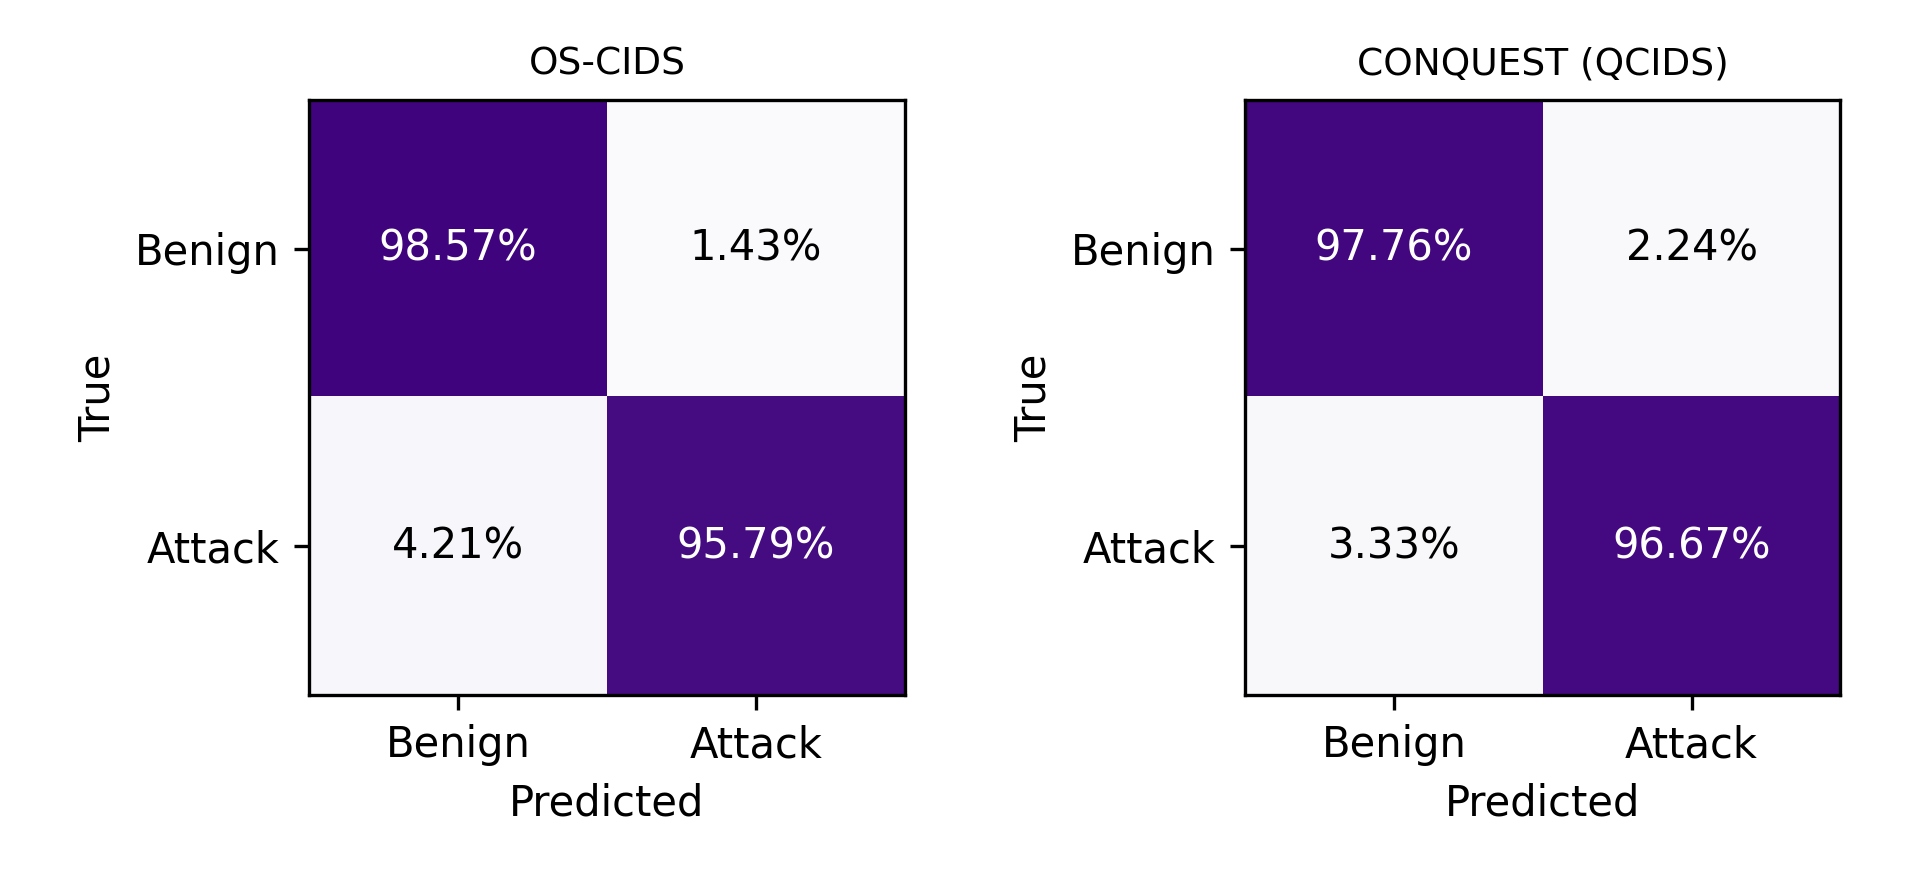
\includegraphics[width=\linewidth]{images/cm_conquest_vs_os.png}
    \caption{\textcolor{red}{Row-normalized confusion matrices of
    OS-CIDS and CONQUEST on the test set, averaged over ten seeds.}}
    
\end{figure}

\setcounter{figure}{4}
\begin{figure}[H]
    \centering
    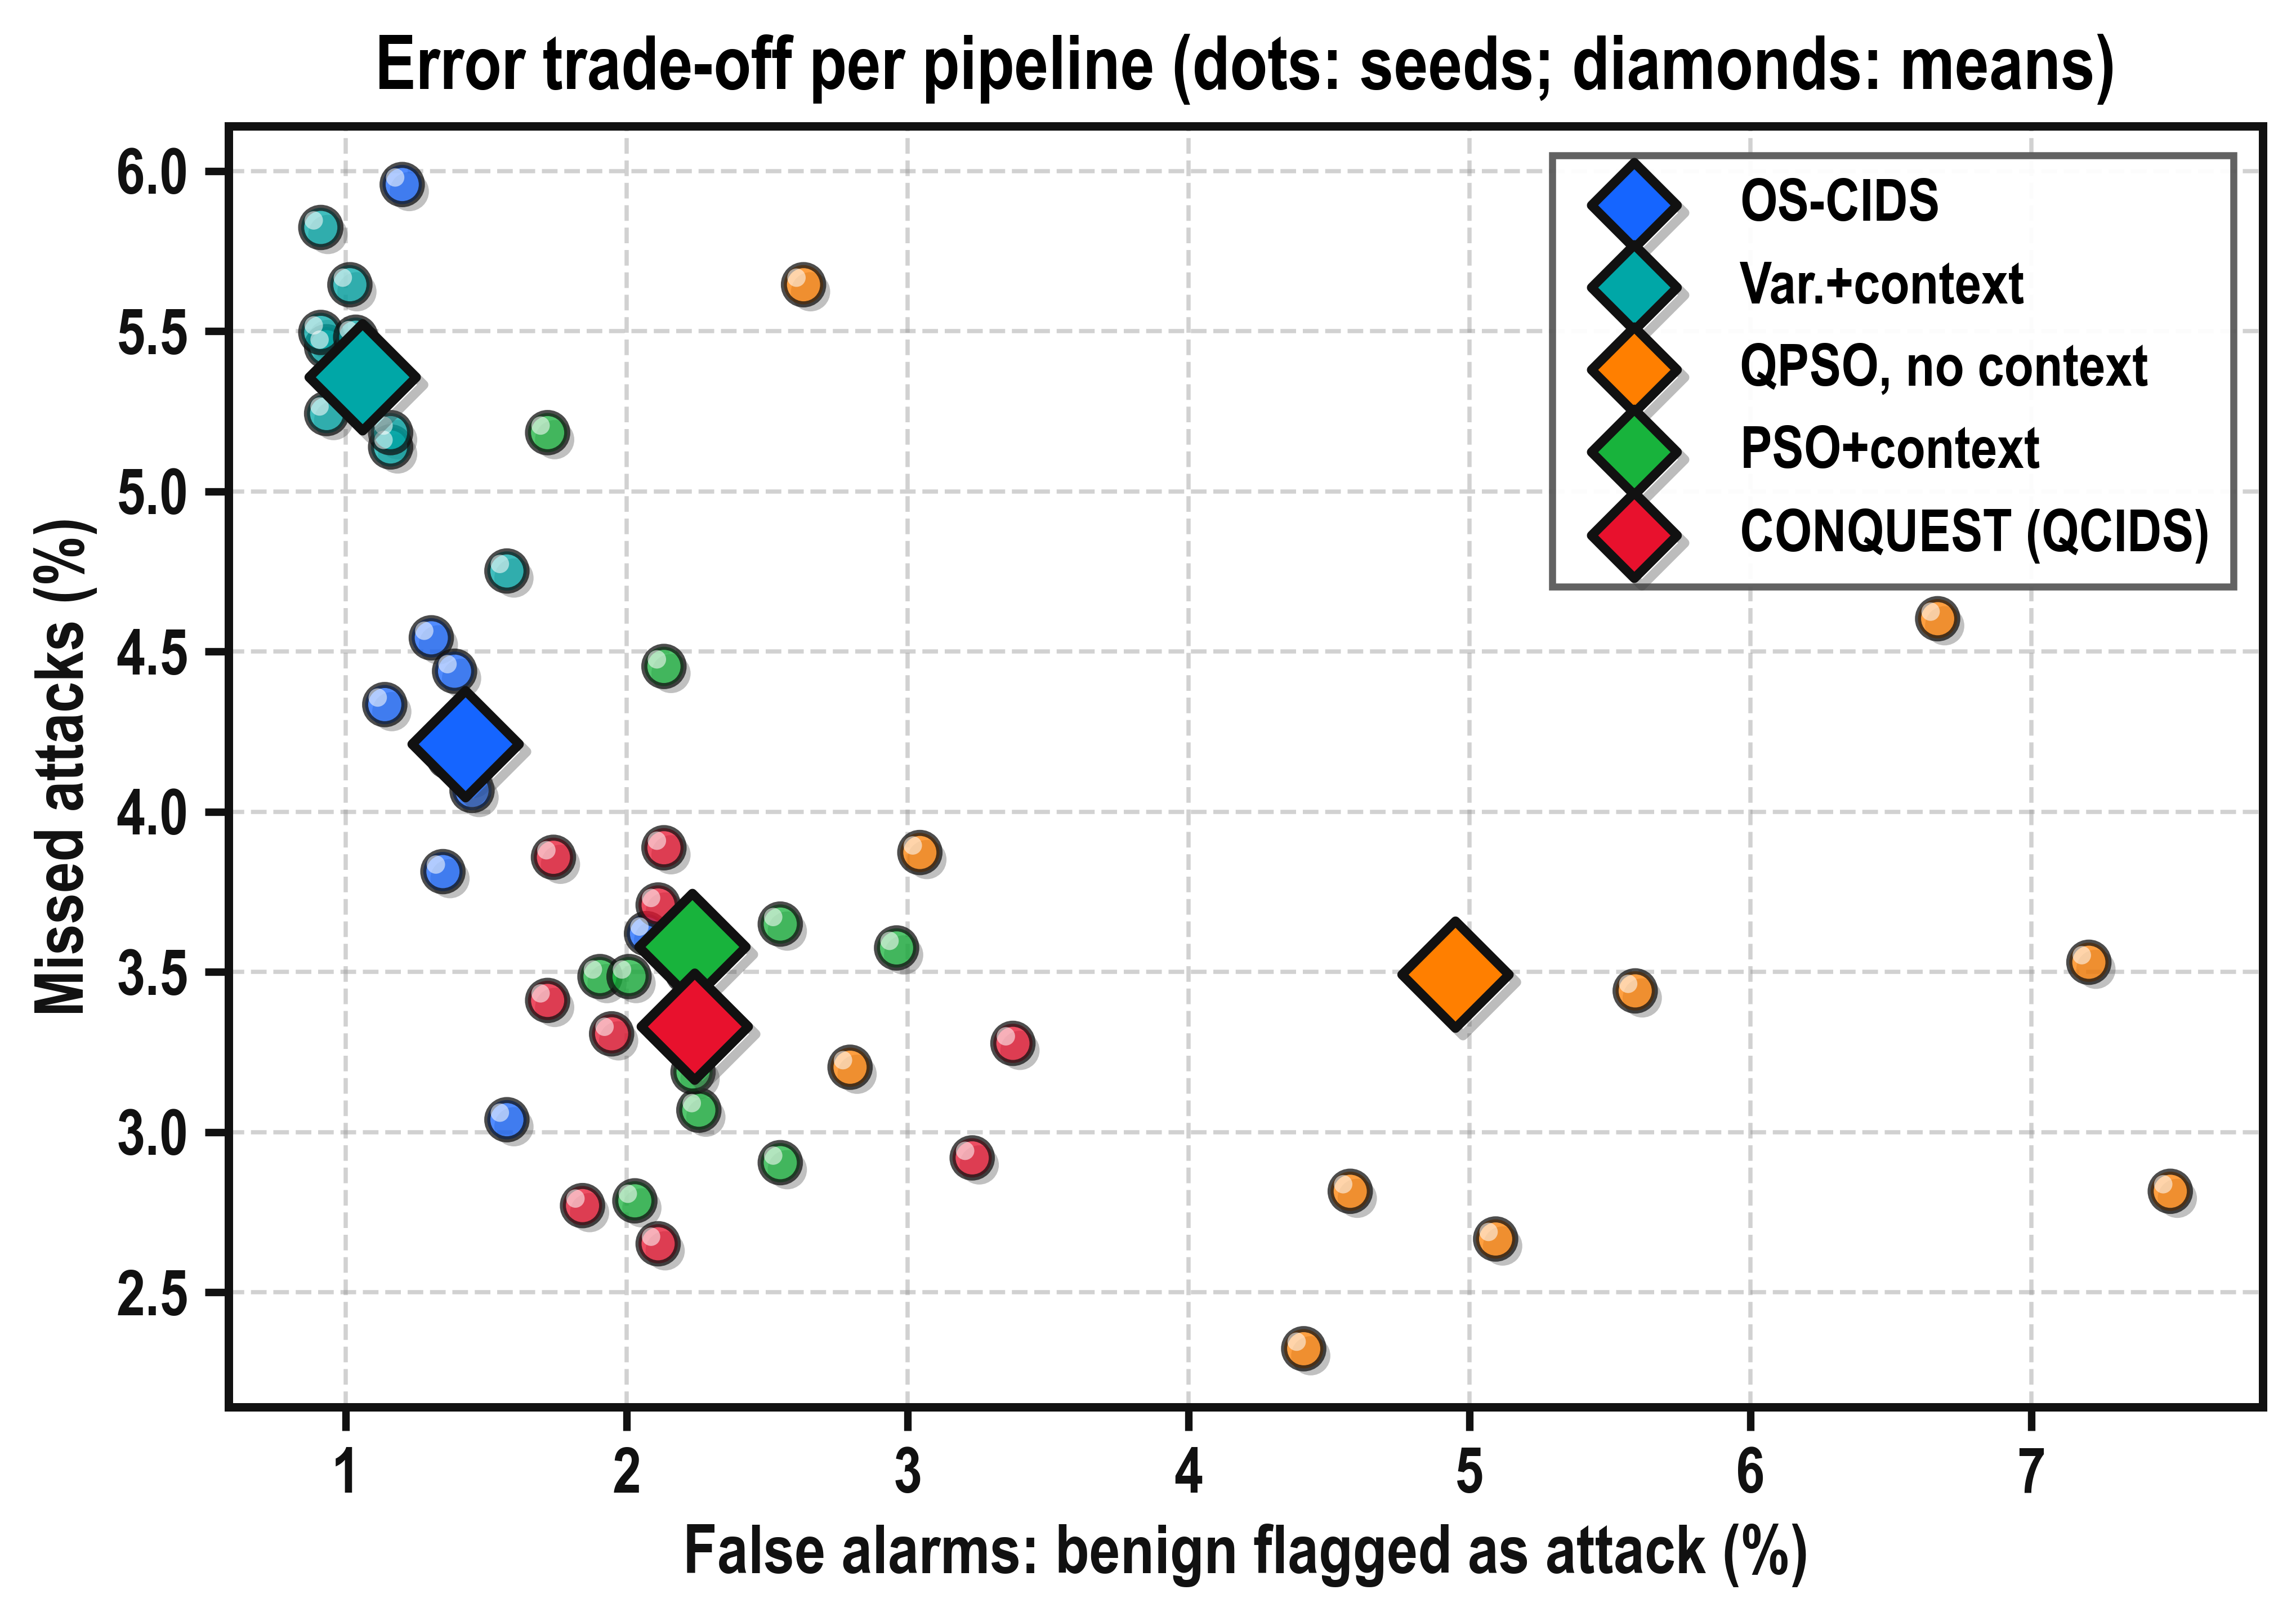
\includegraphics[width=\linewidth]{images/tradeoff_far_md.png}
    \caption{\textcolor{red}{False-alarm rate versus
    missed-attack rate of the five centralized pipelines. Dots:
    individual seeds; diamonds: means.}}
    
\end{figure}

\textcolor{red}{\textbf{Context features versus QPSO.} The
factorial ablation in Table~X separates
the two components, and neither helps on its own. Adding context
features to variance ranking lowers F1 by 0.51\,pp ($p=0.014$),
because variance ranking ignores labels and fills 14 of its 40 slots
with high-variance context counts, displacing informative
packet-length features. Replacing variance ranking by QPSO on static
features alone lowers F1 by 1.07\,pp ($p=0.002$), mainly through more
false alarms. Combined, however, context features and QPSO raise F1
by 1.23\,pp over QPSO alone and by 0.68\,pp over variance ranking with
context (both $p\le0.004$), and their interaction, $+1.74$\,pp
($p=0.002$), is the dominant effect. The gain of CONQUEST therefore
comes from combining context-aware representation with label-aware
selection, which keeps eight context features alongside complementary
static features, as listed in Table~XI.}
\end{excerpt}
\setcounter{table}{9}
\begin{table}[H]
\centering
\scriptsize
\caption{\textcolor{red}{Factorial ablation of context features and QPSO over ten seeds.}}

\color{red}
\setlength{\tabcolsep}{3pt}
\begin{adjustbox}{max width=\linewidth}
\begin{tabular}{lccc}
\hline\toprule
\makecell[l]{F1 / FAR / MD\\(\%)} & \makecell{Variance\\ranking} & \makecell{QPSO\\($Q^{*}{=}6$)} & \makecell{Effect of\\QPSO (pp)} \\
\hline\toprule
Static only & 96.96 / 1.43 / 4.21 & 95.90 / 4.95 / 3.49 & \makecell{$-1.07$\\($p{=}0.002$)} \\
\makecell[l]{Static +\\context} & 96.45 / 1.06 / 5.36 & \textbf{97.13} / 2.24 / \textbf{3.33} & \makecell{$+0.68$\\($p{=}0.002$)} \\
\midrule
\makecell[l]{Effect of\\context (pp)} & \makecell{$-0.51$\\($p{=}0.014$)} & \makecell{$+1.23$\\($p{=}0.004$)} & \makecell{Interaction\\$+1.74$\\($p{=}0.002$)} \\
\hline\toprule
\end{tabular}
\end{adjustbox}
\end{table}

%% ---------------------------------------------------------------------
\review{1.7}{In Section III-A and Fig.~2, manuscript pp.~4--7, the context-aware features are not defined in sufficient detail. The manuscript should report the exact burst, dormant-interval, sliding-window, and transition features, including their dimensions and construction parameters.}

\reply We thank the reviewer for this comment. Section~III-A now defines all
17 context features exactly. Each feature is computed from the history set of
Eq.~(4), the earlier flows of the same source IP within a look-back window
$W$; two windows are used, $W=10$\,s for short bursts and $W=60$\,s for slower
propagation and dormancy, both fixed before the experiments. Table~IV gives,
for every feature, its group (burst, dormant interval, diversity, or
transition), its formula, its window, its default value when the source has
no earlier flow, and its dimension: six burst, three dormant-interval, four
diversity, and four transition features. Every feature depends only on past
traffic of the same source and uses no labels. The 75 static CICFlowMeter
descriptors and the fields excluded to prevent identity shortcuts are also
listed, and a streaming implementation is verified to give identical values.

\loc{(a) Pages 4--5: Added the static descriptors and the exact context-feature definitions to Section III-A}
\begin{excerpt}
\mshead{III-A}{Data Processing and Context-Aware Feature Representation}


Raw flow records $\mathbf{X}(t)$ are mapped by a seed-controlled,
deterministic preprocessing pipeline $\mathcal{P}$ to a unified
representation
\begin{equation}
\mathbf{X}(t) \xrightarrow{\mathcal{P}}
\mathbf{F}_s \oplus \mathbf{F}_c = \mathbf{Z},
\tag{3}
\end{equation}
where $\mathbf{F}_s$ denotes static flow descriptors and
$\mathbf{F}_c$ context-aware features.
\textcolor{red}{$\mathbf{F}_s$ contains the 75 CICFlowMeter
descriptors: ports, protocol, flow duration, packet and byte counts,
packet-length statistics, inter-arrival times, flag counts, and bulk
and activity statistics. Flow identifiers, IP addresses, and
timestamps are excluded to prevent identity shortcuts. The four
\texttt{Idle} fields are also excluded, because in ACI-IoT they store
absolute epoch timestamps and would leak capture time.}
\end{excerpt}
\begin{excerpt}
$\mathbf{F}_c$ captures burst activity, dormant intervals, and
protocol state transitions that static descriptors alone do not
reveal. A single global seed controls the
\textcolor{black}{measurement} sampling in QPSO and the
weight initialization of the classifier.

\textcolor{red}{Table~IV defines
the 17 context features. Flows are sorted by timestamp, and ties at
the 1\,s resolution keep capture order, so ``earlier'' means a
position $j<i$ in the sorted stream. Let $s_i$, $t_i$, $\pi_i$,
$p_i$, and $a_i$ denote the source IP, timestamp, protocol,
destination port, and destination IP of flow $i$; the source IP
serves only as a grouping key, never as a feature. For a look-back
window $W$, the history of flow $i$ is}
\begin{equation}
\textcolor{red}{\mathcal{H}_W(i)=\{\,j<i:\ s_j=s_i,\ t_j\ge t_i-W\,\},}
\tag{4}
\end{equation}
\textcolor{red}{and $\mathrm{prev}(i)$ is the most recent
earlier flow of the same source. In Table~IV,
$n^{\rm pk}_j$ and $n^{\rm by}_j$ are the packets and bytes of flow
$j$ in both directions, and $\mathbf{1}[\cdot]$ is the indicator
function. Flow $i$ itself is excluded, so
every feature depends only on past traffic of the same source and
uses no labels. Two windows are used: $W=10$\,s for short scanning
and flooding bursts, and $W=60$\,s for slower propagation and
dormancy. Both were fixed before the experiments and not tuned.
Context features are computed on the full chronological stream
before subsampling, so window statistics reflect real traffic
density.}
\end{excerpt}
\setcounter{table}{3}
\begin{table}[H]
\centering
\scriptsize
\caption{\textcolor{red}{Definitions of the 17 context
features. Default is the value used when the source has no earlier
flow.}}

\color{red}
\setlength{\tabcolsep}{6pt}
\renewcommand{\arraystretch}{1.25}
\begin{adjustbox}{max width=\linewidth}
\begin{tabular}{l l >{\raggedright\arraybackslash}p{4.3cm} c c c}
\hline\toprule
\textbf{Group} & \textbf{Feature} & \textbf{Definition} & \textbf{$W$ (s)} & \textbf{Default} & \textbf{Dim.} \\
\hline\toprule
\multirow{3}{*}{Burst}
 & \texttt{n\_flows\_src\_W}    & $|\mathcal{H}_W(i)|$ & 10, 60 & 0 & 2 \\
 & \texttt{pkt\_rate\_src\_W}   & $\sum_{j\in\mathcal{H}_W(i)} n^{\rm pk}_j \,/\, W$ & 10, 60 & 0 & 2 \\
 & \texttt{bytes\_rate\_src\_W} & $\sum_{j\in\mathcal{H}_W(i)} n^{\rm by}_j \,/\, W$ & 10, 60 & 0 & 2 \\
\midrule
\multirow{3}{*}{Dormant interval}
 & \texttt{dt\_prev\_src}     & $t_i-t_{\mathrm{prev}(i)}$ & -- & $10^{6}$ & 1 \\
 & \texttt{dt\_prev\_src\_log} & $\log(1+\texttt{dt\_prev\_src})$ & -- & $\log(1+10^{6})$ & 1 \\
 & \texttt{max\_gap\_src\_60}  & Max.\ gap between consecutive flows in $\mathcal{H}_{60}(i)\cup\{i\}$ & 60 & 60 & 1 \\
\midrule
\multirow{2}{*}{Diversity}
 & \texttt{n\_distinct\_dst\_W}   & $|\{a_j: j\in\mathcal{H}_W(i)\}|$ & 10, 60 & 0 & 2 \\
 & \texttt{n\_distinct\_dport\_W} & $|\{p_j: j\in\mathcal{H}_W(i)\}|$ & 10, 60 & 0 & 2 \\
\midrule
\multirow{4}{*}{Transition}
 & \texttt{proto\_switch}       & $\mathbf{1}[\pi_i\neq\pi_{\mathrm{prev}(i)}]$ & -- & 0 & 1 \\
 & \texttt{dport\_switch}       & $\mathbf{1}[p_i\neq p_{\mathrm{prev}(i)}]$ & -- & 0 & 1 \\
 & \texttt{n\_proto\_switch\_60} & $\sum_{j\in\mathcal{H}_{60}(i)} \texttt{proto\_switch}_j$ & 60 & 0 & 1 \\
 & \texttt{syn\_frac\_src\_60}  & Share of flows in $\mathcal{H}_{60}(i)$ with $\mathrm{SYN}_j>0$ & 60 & 0 & 1 \\
\midrule
\multicolumn{5}{l}{\textbf{Total} (burst 6, dormant interval 3, diversity 4, transition 4)} & \textbf{17} \\
\hline\toprule
\end{tabular}
\end{adjustbox}
\end{table}

%% ---------------------------------------------------------------------
\review{1.8}{In Section III-G, manuscript p.~8, QPSO feature selection is performed on a server-held proxy dataset before federated training. The authors should explain the origin and representativeness of this dataset and clarify how this centralized step is compatible with the stated data-sovereignty motivation. The effect of using one global mask for non-IID clients should also be evaluated.}

\reply We thank the reviewer for raising this point. \textit{Origin and
representativeness:} the proxy set is a labelled 5\% subset of the training
split (2{,}750 flows), made of evenly spaced contiguous chunks so that it spans
the capture period; it contains 54\% attacks of five types and is withheld
from all clients. It models the small reference capture that a mission
operator typically owns, for example from its own test range or a public
benchmark. \textit{Compatibility with data sovereignty:} the proxy set never
contains client traffic, and only the resulting feature indices are
broadcast. As an alternative that needs no server-held data, a vote mode was
added, in which each client runs QPSO locally and sends only its selected
indices. \textit{Effect of one global mask:} the proxy and vote masks were
compared with an oracle mask built on all pooled training data under
quantity skew and Dirichlet $\alpha=0.1$. A mask built without pooling data
costs at most 0.51\,pp of global F1 relative to the oracle, and the worst
client is not systematically worse off, with a worst-client F1 of
96.2--97.6\% in all six settings. Table~VIII summarizes what each mode
reveals to the server.

\loc{(a) Page 10: Added the proxy set and the mask-construction modes to Section III-G}
\begin{excerpt}
\mshead{III-G}{Federated Learning Protocol and Convergence Monitoring}


CONQUEST is trained by horizontal federated learning (HFL) with $K$
clients. QPSO feature selection runs before federation on a
server-held proxy set, and the resulting mask $\mathbf{m}^{*}$ is
broadcast to all clients before training begins.
\textcolor{red}{The proxy set is a labelled 5\% subset of
$\mathcal{D}_{\rm tr}$, made of evenly spaced contiguous chunks so
that it spans the capture period, and it is withheld from all
clients. It models the small reference capture that a mission
operator typically owns, for example from its own test range or a
public benchmark, and it never contains client traffic. Because one
global mask may suit non-IID clients poorly, three mask-construction
modes are compared. In the default \textit{proxy} mode, QPSO runs on
the proxy set. In the \textit{vote} mode, each client runs QPSO on its
own data and sends only its $k$ selected indices, and the server
keeps the $k$ most frequently selected features. The
\textit{central} mode runs QPSO on the pooled $\mathcal{D}_{\rm tr}$;
it violates data locality and serves only as an oracle reference.}
\end{excerpt}

\loc{(b) Page 17: Added the evaluation of one global mask for non-IID clients to Section IV-C}
\begin{excerpt}
\mshead{IV-C}{Federated Robustness Under Heterogeneous Mission Deployments}


Fig.~10 and
Table~XVI report whether CONQUEST
remains viable when training data are distributed across
heterogeneous clients.

\setcounter{figure}{9}
\begin{figure}[H]
    \centering
    \includegraphics[width=0.9\linewidth]{images/fl_results.png}
    \caption{\textcolor{red}{Federated CONQUEST: (a)~global F1 per round, (b)~per-client F1, (c)~number of clients, and (d)~mask construction.}}
    
\end{figure}

\setcounter{table}{15}
\begin{table}[H]
\centering
\caption{\textcolor{red}{Federated CONQUEST under one configuration, averaged over three seeds.}}

\color{red}
\setlength{\tabcolsep}{4pt}
\renewcommand{\arraystretch}{1.05}
\begin{adjustbox}{max width=\linewidth}
\begin{tabular}{lcccccc}
\hline\toprule
\textbf{Setting} & \textbf{Global F1 (\%)} & \textbf{AUC} & \textbf{Min-F1 (\%)} & \textbf{Dispersion (pp)} & \textbf{Max MD (\%)} & \textbf{$R_{99}$} \\
\hline\toprule
\multicolumn{7}{l}{\textit{Heterogeneity (FedAvg, proxy mask, $K{=}5$)}} \\
IID & 96.77$\pm$0.10 & 0.9905 & 96.61 & 0.59 & 4.73 & 11.3 \\
Label skew & 86.59$\pm$6.95 & 0.9863 & 83.50 & 6.37 & 44.52 & 5.0 \\
Quantity skew & 96.66$\pm$0.38 & 0.9914 & 96.37 & 0.66 & 4.35 & 7.3 \\
Dirichlet $\alpha{=}0.1$ & 96.68$\pm$0.37 & 0.9906 & 97.63 & 0.54 & 7.55 & 7.7 \\
Dirichlet $\alpha{=}0.3$ & 96.34$\pm$0.60 & 0.9905 & 97.22 & 0.72 & 6.87 & 9.0 \\
Dirichlet $\alpha{=}0.5$ & 96.49$\pm$0.38 & 0.9900 & 96.61 & 0.84 & 4.74 & 7.7 \\
Dirichlet $\alpha{=}1.0$ & 96.94$\pm$0.13 & 0.9907 & 96.56 & 0.82 & 5.00 & 10.0 \\
\midrule
\multicolumn{7}{l}{\textit{Aggregator (quantity skew, $K{=}5$)}} \\
FedAvg & 96.66$\pm$0.38 & 0.9914 & 96.37 & 0.66 & 4.35 & 7.3 \\
SCAFFOLD & 96.56$\pm$0.45 & 0.9887 & 96.28 & 0.71 & 5.27 & 13.7 \\
FLAME & 96.77$\pm$0.10 & 0.9893 & 96.48 & 0.64 & 4.69 & 16.3 \\
\midrule
\multicolumn{7}{l}{\textit{Number of clients (quantity skew, FedAvg)}} \\
$K{=}5$ & 96.66$\pm$0.38 & 0.9914 & 96.37 & 0.66 & 4.35 & 7.3 \\
$K{=}10$ & 96.71$\pm$0.06 & 0.9903 & 97.10 & 0.60 & 3.73 & 10.7 \\
$K{=}20$ & 96.25$\pm$0.05 & 0.9889 & 94.65 & 1.03 & 8.03 & 16.0 \\
\midrule
\multicolumn{7}{l}{\textit{Mask construction (quantity skew)}} \\
Proxy & 96.66$\pm$0.38 & 0.9914 & 96.37 & 0.66 & 4.35 & 7.3 \\
Vote & 97.17$\pm$0.21 & 0.9917 & 96.82 & 0.56 & 3.82 & 7.3 \\
Central (oracle) & 97.17$\pm$0.18 & 0.9921 & 97.07 & 0.50 & 3.62 & 8.0 \\
\midrule
\multicolumn{7}{l}{\textit{Mask construction (Dirichlet $\alpha{=}0.1$)}} \\
Proxy & 96.68$\pm$0.37 & 0.9906 & 97.63 & 0.54 & 7.55 & 7.7 \\
Vote & 96.60$\pm$0.32 & 0.9908 & 96.24 & 0.84 & 3.74 & 7.0 \\
Central (oracle) & 97.06$\pm$0.61 & 0.9922 & 97.51 & 0.59 & 6.72 & 8.0 \\
\midrule
Centralized CONQUEST & 97.13 & 0.9924 & -- & -- & -- & -- \\
\hline\toprule
\end{tabular}
\end{adjustbox}
\end{table}

\textcolor{red}{All federated experiments
use one configuration: 30 rounds, two local epochs, batch size 64,
full participation, the proxy mask unless stated otherwise, and three
seeds. Every row of Table~XVI is
therefore directly comparable.}

\textcolor{black}{\textbf{Heterogeneity.} Under IID,
quantity-skew, and Dirichlet partitions, the global F1 lies between
96.34\% and 96.94\%, within 0.19--0.79\,pp of centralized CONQUEST at
97.13\%; for the quantity-skew stress regime, the gap is 0.47\,pp.
These regimes also serve every client well: the worst client keeps an
F1 of at least 96.37\%, and the inter-client dispersion stays below
0.9\,pp. Quantity skew and IID differ by only 0.11\,pp. Label skew is the one
damaging regime: the global F1 falls to $86.59\pm6.95\%$, the worst
client to 83.50\%, and one attack-dominated client misses 44.5\% of
its attacks. Fig.~10(a) shows the mechanism:
the global F1 peaks near 94\% around round 9 and then oscillates
downward, as clients that see almost only one class pull the shared
model in opposite directions, a phenomenon known as client drift.
Convergence is fast in the other regimes, with $R_{99}$ between 7.3
and 11.3 rounds.}

\textcolor{red}{\textbf{Aggregation
strategy.} Under quantity skew, FedAvg, SCAFFOLD, and FLAME reach
96.66\%, 96.56\%, and 96.77\% F1. They differ by at most 0.21\,pp,
within one seed standard deviation, and all keep the worst client
above 96.2\%. FedAvg converges fastest, with $R_{99}$ of 7.3 rounds
against 13.7 and 16.3, so it remains the default.}

\textcolor{black}{\textbf{Number of clients.} Splitting the
same training data among 5, 10, and 20 quantity-skewed clients gives a
global F1 of 96.66\%, 96.71\%, and 96.25\%
(Fig.~10(c)). Larger federations of smaller
clients converge more slowly, with $R_{99}$ of 7.3, 10.7, and 16.0
rounds, and widen the tail: with 20 clients, the worst client drops to
94.65\% F1 and misses up to 8.03\% of its attacks. CONQUEST therefore
scales to at least 20 clients with a small cost in global F1,
0.41\,pp, but a noticeable cost for the weakest client, which
motivates the tail-aware reporting adopted here.}

\textcolor{red}{\textbf{Global mask for non-IID clients.}
The proxy set used for server-side QPSO contains 2{,}750 training
flows, 5\% of $\mathcal{D}_{\rm tr}$, with 54\% attacks of five types,
and it is never given to a client. Building the global mask from this
proxy, from client votes, or from all pooled training data, an oracle
that violates data locality, gives 96.66\%, 97.17\%, and 97.17\%
global F1 under quantity skew, and 96.68\%, 96.60\%, and 97.06\% under
Dirichlet $\alpha=0.1$ (Fig.~10(d)). A
global mask built without pooling data therefore costs at most
0.51\,pp relative to the oracle, and the worst client is not
systematically worse off, with a worst-client F1 of 96.2--97.6\%
across all six settings. Clients largely agree on what matters: in
vote mode, 38 to 43 features are each chosen by at least three of the
five clients, nearly as many as the 40 slots of the mask. Voting needs no server-held data and,
as Table~VIII shows, reveals only feature indices,
which makes it the preferred mode when no suitable proxy data exist.}
\end{excerpt}

%% ---------------------------------------------------------------------
\review{1.9}{In Section IV-C and Table VIII, manuscript pp.~11--13, FedAvg under quantity-skew reports F1=0.910 in one block and F1=0.869 in another. The reason for this discrepancy is unclear. The authors should specify whether the partitions, seeds, initialization, and training settings differ across these experiments.}

\reply We thank the reviewer for noticing this discrepancy. Its cause was a
difference in training settings: the aggregator comparison used 8 rounds
with one local epoch, the heterogeneity sweep 15 rounds, and the extended run
60 rounds, which led to two different FedAvg results for the same quantity-skew
partition. All federated experiments have been re-run with one configuration:
30 rounds, two local epochs, batch size 64, full participation, the proxy mask
unless stated otherwise, and three seeds. Partitions are built from
contiguous 250-flow chunks of the training split with fixed seeds, so every
row of Table~XVI uses identical partitions, seeds, and initialization and is
directly comparable; FedAvg under quantity skew now reaches
$96.66\pm0.38\%$ F1 in every comparison. SCAFFOLD and FLAME were
re-implemented following their published algorithms, and convergence is now
measured by $R_{99}$, because a 90\% threshold is reached in the first round
in every regime.

\loc{(a) Page 11: Added one configuration for all federated experiments to Section III-G}
\begin{excerpt}
\mshead{III-G}{Federated Learning Protocol and Convergence Monitoring}


CONQUEST is trained by horizontal federated learning (HFL) with $K$
clients. QPSO feature selection runs before federation on a
server-held proxy set, and the resulting mask $\mathbf{m}^{*}$ is
broadcast to all clients before training begins.
\textcolor{black}{The proxy set is a labelled 5\% subset of
$\mathcal{D}_{\rm tr}$, made of evenly spaced contiguous chunks so
that it spans the capture period, and it is withheld from all
clients. It models the small reference capture that a mission
operator typically owns, for example from its own test range or a
public benchmark, and it never contains client traffic. Because one
global mask may suit non-IID clients poorly, three mask-construction
modes are compared. In the default \textit{proxy} mode, QPSO runs on
the proxy set. In the \textit{vote} mode, each client runs QPSO on its
own data and sends only its $k$ selected indices, and the server
keeps the $k$ most frequently selected features. The
\textit{central} mode runs QPSO on the pooled $\mathcal{D}_{\rm tr}$;
it violates data locality and serves only as an oracle reference.}
The mask encodes only feature indices, so no raw traffic or labels
are exposed. Each client $k$ holds
$\mathcal{D}_k=\{(\mathbf{Z}_{k,i},y_{k,i})\}_{i=1}^{N_k}$, built with
the same preprocessing pipeline. The global objective is
\begin{equation}
\begin{aligned}
&\min_{\theta}\,F(\theta)=\sum_{k=1}^{K}\frac{N_k}{N}F_k(\theta),\\
&F_k(\theta)=\frac{1}{N_k}\sum_{i=1}^{N_k}
\ell\!\left(f_\theta(\mathbf{Z}_{k,i}),y_{k,i}\right).
\end{aligned}
\tag{19}
\end{equation}
In each round $r$, the server broadcasts $\theta^{(r)}$, each
participating client $k\in\mathcal{S}_r$ performs $E=2$ local epochs
on $\mathcal{D}_k$, and the server aggregates the local models with
FedAvg:
\begin{equation}
\theta^{(r+1)}=\sum_{k\in\mathcal{S}_r}
\frac{N_k}{\sum_{j\in\mathcal{S}_r}N_j}
\,\theta_k^{(r+1)}.
\tag{20}
\end{equation}

Only model parameters are transmitted; no raw traffic, labels,
or feature vectors are exchanged. \textcolor{black}{We assume
an honest-but-curious server and honest clients. Keeping raw traffic
local guarantees data locality, not formal privacy: plain FedAvg
updates can still leak information about a client's traffic through
membership inference, property inference, or gradient inversion.
Table~VIII lists what each party can observe and
how it is protected. Two standard mechanisms close these gaps without
changing the model or the mask. First, \textit{secure aggregation}
with additive pairwise masking lets the server learn only the sum of
the client updates. The masks cancel exactly in the sum, so the
aggregated model and its detection performance are identical to plain
FedAvg; the cost is extra communication and key agreement in each
round. Weighted averaging is preserved by having each client send
$N_k\,\Delta\theta_k$ and $N_k$ through the same protocol. Second,
\textit{client-level differential privacy} (DP-FedAvg) bounds what
the released model reveals about any one client. Each update is
clipped to $\ell_2$ norm $C$, the clipped updates are averaged with
the fixed denominator $K$, and Gaussian noise
$\mathcal{N}(0,(zC/K)^2\mathbf{I})$ is added. With full participation
over $R$ rounds, the R\'enyi-DP accountant gives
$\varepsilon(\delta)=\min_{\alpha>1}\bigl[R\alpha/(2z^2)+
\log(1/\delta)/(\alpha-1)\bigr]$. DP-FedAvg is evaluated on the
quantity-skew regime with $K=5$, $R=30$, and $\delta=10^{-5}$, using
noise multipliers $z=1$, 3, and 8, which give $\varepsilon=41.3$,
10.4, and 3.5. The clip norm $C=0.215$ is fixed before any private
run as the median client-update norm of the non-private FedAvg runs.}
Blockchain-based mechanisms can additionally secure and audit the
exchange of IoT data among parties that do not fully trust one
another~{[39]}; they complement, but lie outside,
the federated protocol evaluated here.
\textcolor{black}{Client-level DP is not usable at $K=5$. Over
three seeds, the final global F1 falls from 96.66\% without DP to
$47.2\pm5.1\%$ at $z=1$ with AUC 0.59, $42.8\pm0.0\%$ at $z=3$, and
$36.7\pm10.4\%$ at $z=8$; at $z=3$ and $z=8$ the AUC is 0.50, i.e.,
chance level. Because only five updates are averaged, the noise
standard deviation $zC/K$ is of the same order as the clipped mean
update. Client-level DP is designed for federations of hundreds to
thousands of clients, where this ratio shrinks as $1/K$. For mission
federations with a handful of sites, secure aggregation, which leaves
the aggregated model unchanged, is therefore the practical protection
of individual updates, while formal DP remains a target for larger
federations or for record-level DP-SGD within each site.}

\setcounter{table}{7}
\begin{table}[H]
\centering
\scriptsize
\caption{\textcolor{black}{Privacy scope of federated CONQUEST
under an honest-but-curious server. SecAgg: secure aggregation; DP:
client-level differential privacy.}}

\color{black}
\setlength{\tabcolsep}{3pt}
\renewcommand{\arraystretch}{1.08}
\begin{adjustbox}{max width=\linewidth}
\begin{tabular}{p{1.7cm} p{1.6cm} p{1.75cm} p{1.75cm}}
\hline\toprule
\textbf{Information} & \textbf{Visible to} & \textbf{Protection in CONQUEST} & \textbf{Optional mechanism} \\
\hline\toprule
Raw flows, labels & Owning client only & Never transmitted & -- \\
Individual model updates & Server, every round & None (plain FedAvg) & SecAgg (server sees only the sum) \\
Aggregated global model & All clients & None & DP (bounded per-client influence) \\
Client data size $N_k$ & Server (FedAvg weights) & None & SecAgg on $N_k$; uniform mean in DP \\
Feature mask, proxy mode & Server (computed on its own proxy data) & No client data used & -- \\
Feature mask, vote mode & Server sees each client's $k$ indices & Indices only, no data & SecAgg on vote counts \\
\hline\toprule
\end{tabular}
\end{adjustbox}
\end{table}

\textcolor{red}{All federated experiments use one
configuration: 30 rounds, two local epochs, full participation, batch
size 64, and $K=5$ clients unless stated otherwise. Clients are built
from contiguous 250-flow chunks of $\mathcal{D}_{\rm tr}$, so no flow
or window is shared between clients. The chronologically last 15\% of
each client's chunks are excluded from its training. Global metrics
are computed on $\mathcal{D}_{\rm te}$.}
\end{excerpt}
\begin{excerpt}
\textcolor{red}{Per-client metrics
evaluate the final global model on a client-specific test set drawn
from $\mathcal{D}_{\rm te}$. For each client, up to 2{,}000 test
windows are sampled so that their class and attack-type proportions
match those of the client's training windows, restricted to the
attack types present in $\mathcal{D}_{\rm te}$; these types cover at
least 80\% of every client's training mix. This measures how well the
shared model serves each client's own traffic mix, with test sets
large enough to be reliable. The client's held-out chunks are not
used for reporting, because the temporal clustering of ACI-IoT
attacks makes them small and often single-class. Client-count
sensitivity repeats the quantity-skew experiment with $K=5$, 10, and
20.}

\textcolor{red}{Two aggregators are compared with FedAvg.
SCAFFOLD~{[40]} corrects the client drift
caused by non-IID data, and FLAME~{[41]} filters
anomalous updates, which serves as a robustness reference beyond the
honest-client assumption. SCAFFOLD follows
option~II of its original formulation. Server and client control variates $\mathbf{c}$ and
$\mathbf{c}_k$, initialized to zero, correct every local gradient by
$\mathbf{c}-\mathbf{c}_k$, and after local training
$\mathbf{c}_k^{+}=\mathbf{c}_k-\mathbf{c}+(\theta^{(r)}-
\theta_k^{(r+1)})/(\tau\,\eta_{\rm eff})$, where $\tau$ is the number
of local steps. Because local updates use momentum $\mu=0.9$, the
effective step size $\eta_{\rm eff}=\eta/(1-\mu)$ is used; with the
raw $\eta$, the control variates are overestimated tenfold and
training diverges. FLAME clusters the client
updates with HDBSCAN, a density-based hierarchical clustering
method~{[42]}, on pairwise cosine distances, with minimum cluster size
$\lfloor K/2\rfloor+1$, and admits the largest cluster. It clips the
admitted updates to the median $\ell_2$ norm of all updates, averages
them, and adds Gaussian noise with standard deviation $10^{-3}$ times
the median norm.}
\end{excerpt}

\loc{(b) Pages 15--17: Revised the federated results in Section IV-C}
\begin{excerpt}
\mshead{IV-C}{Federated Robustness Under Heterogeneous Mission Deployments}


Fig.~10 and
Table~XVI report whether CONQUEST
remains viable when training data are distributed across
heterogeneous clients.

\setcounter{figure}{9}
\begin{figure}[H]
    \centering
    \includegraphics[width=0.9\linewidth]{images/fl_results.png}
    \caption{\textcolor{red}{Federated CONQUEST: (a)~global F1 per round, (b)~per-client F1, (c)~number of clients, and (d)~mask construction.}}
    
\end{figure}

\setcounter{table}{15}
\begin{table}[H]
\centering
\caption{\textcolor{red}{Federated CONQUEST under one configuration, averaged over three seeds.}}

\color{red}
\setlength{\tabcolsep}{4pt}
\renewcommand{\arraystretch}{1.05}
\begin{adjustbox}{max width=\linewidth}
\begin{tabular}{lcccccc}
\hline\toprule
\textbf{Setting} & \textbf{Global F1 (\%)} & \textbf{AUC} & \textbf{Min-F1 (\%)} & \textbf{Dispersion (pp)} & \textbf{Max MD (\%)} & \textbf{$R_{99}$} \\
\hline\toprule
\multicolumn{7}{l}{\textit{Heterogeneity (FedAvg, proxy mask, $K{=}5$)}} \\
IID & 96.77$\pm$0.10 & 0.9905 & 96.61 & 0.59 & 4.73 & 11.3 \\
Label skew & 86.59$\pm$6.95 & 0.9863 & 83.50 & 6.37 & 44.52 & 5.0 \\
Quantity skew & 96.66$\pm$0.38 & 0.9914 & 96.37 & 0.66 & 4.35 & 7.3 \\
Dirichlet $\alpha{=}0.1$ & 96.68$\pm$0.37 & 0.9906 & 97.63 & 0.54 & 7.55 & 7.7 \\
Dirichlet $\alpha{=}0.3$ & 96.34$\pm$0.60 & 0.9905 & 97.22 & 0.72 & 6.87 & 9.0 \\
Dirichlet $\alpha{=}0.5$ & 96.49$\pm$0.38 & 0.9900 & 96.61 & 0.84 & 4.74 & 7.7 \\
Dirichlet $\alpha{=}1.0$ & 96.94$\pm$0.13 & 0.9907 & 96.56 & 0.82 & 5.00 & 10.0 \\
\midrule
\multicolumn{7}{l}{\textit{Aggregator (quantity skew, $K{=}5$)}} \\
FedAvg & 96.66$\pm$0.38 & 0.9914 & 96.37 & 0.66 & 4.35 & 7.3 \\
SCAFFOLD & 96.56$\pm$0.45 & 0.9887 & 96.28 & 0.71 & 5.27 & 13.7 \\
FLAME & 96.77$\pm$0.10 & 0.9893 & 96.48 & 0.64 & 4.69 & 16.3 \\
\midrule
\multicolumn{7}{l}{\textit{Number of clients (quantity skew, FedAvg)}} \\
$K{=}5$ & 96.66$\pm$0.38 & 0.9914 & 96.37 & 0.66 & 4.35 & 7.3 \\
$K{=}10$ & 96.71$\pm$0.06 & 0.9903 & 97.10 & 0.60 & 3.73 & 10.7 \\
$K{=}20$ & 96.25$\pm$0.05 & 0.9889 & 94.65 & 1.03 & 8.03 & 16.0 \\
\midrule
\multicolumn{7}{l}{\textit{Mask construction (quantity skew)}} \\
Proxy & 96.66$\pm$0.38 & 0.9914 & 96.37 & 0.66 & 4.35 & 7.3 \\
Vote & 97.17$\pm$0.21 & 0.9917 & 96.82 & 0.56 & 3.82 & 7.3 \\
Central (oracle) & 97.17$\pm$0.18 & 0.9921 & 97.07 & 0.50 & 3.62 & 8.0 \\
\midrule
\multicolumn{7}{l}{\textit{Mask construction (Dirichlet $\alpha{=}0.1$)}} \\
Proxy & 96.68$\pm$0.37 & 0.9906 & 97.63 & 0.54 & 7.55 & 7.7 \\
Vote & 96.60$\pm$0.32 & 0.9908 & 96.24 & 0.84 & 3.74 & 7.0 \\
Central (oracle) & 97.06$\pm$0.61 & 0.9922 & 97.51 & 0.59 & 6.72 & 8.0 \\
\midrule
Centralized CONQUEST & 97.13 & 0.9924 & -- & -- & -- & -- \\
\hline\toprule
\end{tabular}
\end{adjustbox}
\end{table}

\textcolor{red}{All federated experiments
use one configuration: 30 rounds, two local epochs, batch size 64,
full participation, the proxy mask unless stated otherwise, and three
seeds. Every row of Table~XVI is
therefore directly comparable.}

\textcolor{red}{\textbf{Heterogeneity.} Under IID,
quantity-skew, and Dirichlet partitions, the global F1 lies between
96.34\% and 96.94\%, within 0.19--0.79\,pp of centralized CONQUEST at
97.13\%; for the quantity-skew stress regime, the gap is 0.47\,pp.
These regimes also serve every client well: the worst client keeps an
F1 of at least 96.37\%, and the inter-client dispersion stays below
0.9\,pp. Quantity skew and IID differ by only 0.11\,pp. Label skew is the one
damaging regime: the global F1 falls to $86.59\pm6.95\%$, the worst
client to 83.50\%, and one attack-dominated client misses 44.5\% of
its attacks. Fig.~10(a) shows the mechanism:
the global F1 peaks near 94\% around round 9 and then oscillates
downward, as clients that see almost only one class pull the shared
model in opposite directions, a phenomenon known as client drift.
Convergence is fast in the other regimes, with $R_{99}$ between 7.3
and 11.3 rounds.}
\end{excerpt}

%% ---------------------------------------------------------------------
\review{1.10}{In Sections III-C--III-D and IV-B, manuscript pp.~6 and 10--11, the latency definitions are inconsistent. The paper reports approximately 3.60\,s inference time but 61.2\,ms end-to-end latency for $Q=6$, while Eq.~(15) includes QPSO even though QPSO is said to be excluded from deployment inference. These quantities should be clearly separated and defined.}

\reply We thank the reviewer and agree that these quantities were not
separated. The 3.60\,s inference time was the total time to classify the
whole test set of about 12{,}000 windows, not a per-detection latency; it
corresponds to about 0.3\,ms per window. The 61.2\,ms end-to-end latency, the
latency-budget share, and the per-$Q$ memory values came from a decomposition
that wrongly placed QPSO on the inference path. Section~III-D now separates
two cost categories. The \textit{offline training cost}, which includes the
QPSO search, is incurred once per model and never on the detection path. The
\textit{online deployment cost} is the per-window latency of Eq.~(15), the
incremental context-feature update plus one forward pass of the classifier;
QPSO does not appear in it. All deployment costs were re-measured in
isolation: CONQUEST classifies one window in a median of 2.98\,ms (95th
percentile 4.55\,ms), batched classification costs 0.25\,ms per window, the
context update adds 16\,$\mu$s per flow, the whole test set takes 3.23\,s, and
the inference process peaks at 541\,MB. These costs are practically the same
for $Q=1$, 6, and 8, which confirms that the inference cost does not depend
on $Q$ (Eq.~(1)).

\loc{(a) Page 9: Added the separation of offline and online costs to Section III-D}
\begin{excerpt}
\mshead{III-D}{Latency-Aware Design and Resource Constraints}


\textcolor{red}{CONQUEST distinguishes two cost
categories, which are measured and reported separately.}

\textcolor{red}{\textit{Offline training cost} is incurred
once per model and never on the detection path. It consists of the
QPSO search time $T_{\rm QPSO}(Q)$ and the classifier training time
$T_{\rm train}$, both measured as wall-clock time.}

\textcolor{red}{\textit{Online deployment cost} is incurred
for every classified window. The per-window latency is}
\begin{equation}
\textcolor{red}{\mathcal{L}_{\rm infer} =
\mathcal{L}_{\rm ctx} + \mathcal{L}_{\rm clf},}
\tag{15}
\end{equation}
\textcolor{red}{where $\mathcal{L}_{\rm ctx}$ is the
incremental context-feature update for a newly arrived flow,
including normalization and masking, and $\mathcal{L}_{\rm clf}$ is
one forward pass of the classifier.}
\end{excerpt}

\loc{(b) Pages 15--16: Revised the measured deployment cost in Section IV-B}
\begin{excerpt}
\mshead{IV-B}{Latency-Aware Performance Under Quantum-Inspired Optimization}


\textcolor{black}{Because detection is insensitive to $Q$,
this subsection examines whether $Q$ affects deployment cost and
whether the selected operating point meets mission-edge
constraints.}

\textcolor{red}{Table~XV
and Fig.~9 report the deployment cost, measured in
isolation on the CPU-only host, for the pipelines of
Section~IV-A and for five variants of
CONQUEST: the consensus mask, register sizes $Q=1$ and 8 instead of
$Q^{*}=6$, and feature budgets $k=20$ and 10 instead of 40. Classifying one window of ten flows
takes CONQUEST a median of 2.98\,ms at batch size 1, with a 95th
percentile of 4.55\,ms. In batches of 64, a window costs 0.25\,ms, or
4{,}004 windows per second. Updating the context features,
normalizing, and masking a newly arrived flow adds 16\,$\mu$s, and the
11{,}544 test windows are classified in 3.23\,s. The inference process
peaks at 541\,MB, within the 1\,GB budget. These costs are practically
the same for every pipeline, at 2.9--3.5\,ms per window and
541--658\,MB, and for $Q=1$, 6, and 8 and $k=10$, 20, and 40, since
the classifier hardly changes with the input width, from 758k to 789k
parameters. This confirms Eq.~(1) empirically. QPSO is a
training-time cost of 1.8\,min per run on the shared host, or
0.4\,min at $k=10$, incurred once before training; the consensus mask
requires ten such runs.}
\end{excerpt}
\setcounter{table}{14}
\begin{table}[H]
\centering
\caption{\textcolor{red}{Deployment cost measured in isolation; medians over seeds, with the number of seeds in parentheses.}}

\color{red}
\setlength{\tabcolsep}{4pt}
\begin{adjustbox}{max width=\linewidth}
\begin{tabular}{lcccccccc}
\hline\toprule
\textbf{Pipeline} & \multicolumn{2}{c}{Latency (ms/window)} & Batched & Test set & Context update & Memory & Params & Selection \\
 & median & p95 & (ms/window) & (s) & ($\mu$s/flow) & (MB) & & (s) \\
\hline\toprule
OS-CIDS (3) & 2.96 & 3.69 & 0.233 & 3.30 & 5.1 & 629 & 789k & 0.0 \\
Var.+context (3) & 2.94 & 3.62 & 0.244 & 3.21 & 15.9 & 638 & 789k & 0.1 \\
PSO+context (3) & 3.02 & 3.77 & 0.244 & 3.31 & 15.9 & 658 & 789k & 76.2 \\
\textbf{CONQUEST ($Q^{*}{=}6$)} (3) & \textbf{2.98} & \textbf{4.55} & \textbf{0.250} & \textbf{3.23} & \textbf{16.2} & \textbf{541} & \textbf{789k} & \textbf{106.8} \\
CONQUEST, consensus mask (3) & 2.93 & 3.70 & 0.238 & 3.15 & 15.8 & 600 & 789k & 0.2 \\
CONQUEST, $Q{=}1$ (1) & 2.93 & 3.65 & 0.250 & 3.47 & 16.5 & 652 & 789k & 96.5 \\
CONQUEST, $Q{=}8$ (1) & 3.47 & 4.31 & 0.250 & 3.29 & 16.3 & 657 & 789k & 109.9 \\
CONQUEST, $k{=}20$ (3) & 3.19 & 4.87 & 0.260 & 3.49 & 16.4 & 650 & 768k & 43.8 \\
CONQUEST, $k{=}10$ (3) & 3.09 & 4.33 & 0.257 & 3.37 & 16.5 & 645 & 758k & 22.8 \\
\hline\toprule
\end{tabular}
\end{adjustbox}
\end{table}
\setcounter{figure}{8}
\begin{figure}[H]
\centering

\includegraphics[width=0.95\linewidth]{images/deployment_cost.png}
\caption{\textcolor{red}{Deployment cost: (a)~latency per window, (b)~batched throughput, and (c)~peak inference memory.}}

\end{figure}

%% ---------------------------------------------------------------------
\review{1.11}{In Section III-C and Table III, manuscript pp.~6--7, the optimizer description is inconsistent: the text states SGD, whereas Table III lists Adam. The manuscript should clearly identify which optimizer was used for each reported result.}

\reply We thank the reviewer and apologize for this inconsistency. Every
reported result uses SGD with Nesterov momentum 0.9 and learning rate
$10^{-3}$, with batch size 32 for centralized training and 64 for the local
updates of federated clients. Adam is not used; the Adam entry in the former
Table~III was carried over from the optimizer comparison of the conference
version, which retained SGD. The implementation table (Table~VI) has been
corrected, and Section~III-C now specifies the full architecture, the loss,
and the stopping rule.

\loc{(a) Page 9: Revised the architecture, loss, and optimizer in Section III-C}
\begin{excerpt}
\mshead{III-C}{LSTM(+VAE) Temporal Classifier}


The QPSO mask $\mathbf{m}^{*}$ is fixed before classifier training,
so feature selection and model training are decoupled. The masked
input $\tilde{\mathbf{z}}=\mathbf{m}^{*}\odot\mathbf{Z}_n$ is passed
to a binary temporal classifier:
\begin{equation}
\hat{\mathbf{y}} = \mathrm{softmax}\bigl(g(\mathbf{u})\bigr),\quad
\mathbf{u} = \textcolor{red}{\begin{cases}
\boldsymbol{\mu}+\boldsymbol{\sigma}\odot\boldsymbol{\epsilon}, & \text{training},\\
\boldsymbol{\mu}, & \text{inference},
\end{cases}}
\tag{13}
\end{equation}
\textcolor{red}{where $\boldsymbol{\mu}$ and
$\log\boldsymbol{\sigma}^2$ are 64-dimensional linear projections of
the final recurrent state and
$\boldsymbol{\epsilon}\sim\mathcal{N}(\mathbf{0},\mathbf{I})$. The
encoder processes windows of $T=10$ flows with an LSTM of 256 units,
two-head self-attention with a residual connection, and a second LSTM
of 128 units, each followed by layer normalization; both LSTMs use
dropout 0.2. The head $g$ consists of dense layers of 64 and 32 ReLU
units, with dropout 0.2 after the first, and a two-unit output layer.
The LSTMs capture the temporal dependencies of cyberworm state
transitions. The variational latent acts only as a stochastic
regularizing bottleneck: it has no reconstruction decoder and is not
used as an anomaly score. At inference, the latent mean is used, so
predictions are deterministic.}
\end{excerpt}
\begin{excerpt}
 The training objective is
\begin{equation}
\mathcal{L}_{\rm total} = \textcolor{red}{\mathcal{L}_{\rm CE}
+ \gamma\,D_{\rm KL}\!\left(q(\mathbf{u}|\tilde{\mathbf{z}}_{1:T})\,\|\,
\mathcal{N}(\mathbf{0},\mathbf{I})\right)},
\tag{14}
\end{equation}
\textcolor{red}{where $\mathcal{L}_{\rm CE}$ is the
two-class cross-entropy and $\gamma=10^{-3}$.}
\textcolor{red}{The parameters $\theta$ are optimized with
SGD with Nesterov momentum 0.9, learning rate $10^{-3}$, and batch
size 32. The same optimizer is used in every reported experiment:
all centralized configurations, the $Q$ ablation, the budget and
selector comparisons, and the local updates of all federated clients,
which use batch size 64.} \textcolor{black}{\textcolor{red}{Training runs
for at most 35 epochs. Early stopping monitors the validation loss
with patience 6 and restores the best weights, and the learning rate
is halved after 3 epochs without improvement, down to $10^{-6}$.}}
\end{excerpt}

%% =====================================================================
\clearpage
\section*{To Reviewer \#2}

The authors thank the reviewer for the positive assessment of the framework
and for the constructive concerns, which have helped us make the privacy
scope, the scalability, the role of the quantum-inspired search, and the
cost reporting of CONQUEST precise.

%% ---------------------------------------------------------------------
\review{2.1}{The manuscript repeatedly describes CONQUEST as privacy-preserving because raw traffic is retained locally. However, the explicit privacy mechanisms, such as differential privacy, secure aggregation, or protection against inference attacks on model updates, must be addressed to achieve privacy in its true sense.}

\reply We agree with the reviewer. Keeping raw traffic local provides data
locality, not formal privacy, and the manuscript no longer describes
CONQUEST as privacy-preserving on that basis. We have added a threat model,
an honest-but-curious server with honest clients, and Table~VIII lists what
each party can observe and how it is protected. Two mechanisms are then
addressed explicitly. \textit{Secure aggregation} with additive pairwise
masking lets the server learn only the sum of the client updates; because the
masks cancel, the aggregated model, and therefore every reported detection
result, is identical to plain FedAvg. \textit{Client-level differential
privacy} (DP-FedAvg) was implemented and evaluated with noise multipliers
$z=1$, 3, and 8, corresponding to $\varepsilon=41.3$, 10.4, and 3.5 at
$\delta=10^{-5}$. With five clients, the noise is of the same order as the
averaged update, and the F1 falls to 36.7--47.2\%; client-level DP becomes
usable only for federations with many more clients. For mission federations
with a handful of sites, secure aggregation is therefore the practical
protection of individual updates against inference attacks, and the
manuscript states this scope explicitly.

\loc{(a) Page 1: Revised the Introduction to separate data locality from formal privacy}
\begin{excerpt}
\mshead{I}{Introduction}

The rapid digitalization of mission-critical infrastructures spanning
the Internet of Things (IoT), Internet of Vehicles (IoV), and Internet
of Drones (IoD) has expanded the attack surface of networked
systems~{[1, 2]}. AI-aided cyberworms that
adapt autonomously, propagate stealthily, and mimic legitimate
traffic render signature- and rule-based defences increasingly
ineffective~{[3]}. Where delayed or incorrect decisions can
disrupt safety, mobility, or command operations~{[4]},
robust cyberworm detection is both a security requirement and an
operational necessity.

Existing IDS approaches remain limited in this setting.
Signature-driven methods generalize poorly to novel threats, and
statistical anomaly detectors raise many false alarms under noisy,
heterogeneous traffic. Deep learning improves spatio-temporal pattern
recognition~{[5]}, but three challenges persist:
(\textit{i})~optimization degrades in high-dimensional feature spaces;
(\textit{ii})~performance is brittle under non-stationary data; and
(\textit{iii})~centralized training conflicts with the privacy,
sovereignty, and regulatory constraints of distributed missions.

Quantum-inspired optimization targets the first
challenge~{[6, 7]}: QPSO introduces
probabilistic search dynamics \textcolor{black}{that have been reported
to improve exploration over classical metaheuristics}. In IDS,
however, its use remains ad hoc: the effect of the optimizer's
configuration on its search is rarely analyzed, stability is seldom quantified, and
\textcolor{black}{comparisons with classical search at an equal
evaluation budget are missing}. Federated learning (FL) targets the
third challenge by keeping raw traffic local and exchanging only
model updates~{[8]}; \textcolor{red}{on its
own, FL provides data locality rather than formal privacy, because
updates can leak information unless secure aggregation or
differential privacy is added}
\end{excerpt}

\loc{(b) Pages 10--11: Added the threat model, secure aggregation, and differential privacy to Section III-G}
\begin{excerpt}
\mshead{III-G}{Federated Learning Protocol and Convergence Monitoring}


CONQUEST is trained by horizontal federated learning (HFL) with $K$
clients. QPSO feature selection runs before federation on a
server-held proxy set, and the resulting mask $\mathbf{m}^{*}$ is
broadcast to all clients before training begins.
\textcolor{black}{The proxy set is a labelled 5\% subset of
$\mathcal{D}_{\rm tr}$, made of evenly spaced contiguous chunks so
that it spans the capture period, and it is withheld from all
clients. It models the small reference capture that a mission
operator typically owns, for example from its own test range or a
public benchmark, and it never contains client traffic. Because one
global mask may suit non-IID clients poorly, three mask-construction
modes are compared. In the default \textit{proxy} mode, QPSO runs on
the proxy set. In the \textit{vote} mode, each client runs QPSO on its
own data and sends only its $k$ selected indices, and the server
keeps the $k$ most frequently selected features. The
\textit{central} mode runs QPSO on the pooled $\mathcal{D}_{\rm tr}$;
it violates data locality and serves only as an oracle reference.}
The mask encodes only feature indices, so no raw traffic or labels
are exposed. Each client $k$ holds
$\mathcal{D}_k=\{(\mathbf{Z}_{k,i},y_{k,i})\}_{i=1}^{N_k}$, built with
the same preprocessing pipeline. The global objective is
\begin{equation}
\begin{aligned}
&\min_{\theta}\,F(\theta)=\sum_{k=1}^{K}\frac{N_k}{N}F_k(\theta),\\
&F_k(\theta)=\frac{1}{N_k}\sum_{i=1}^{N_k}
\ell\!\left(f_\theta(\mathbf{Z}_{k,i}),y_{k,i}\right).
\end{aligned}
\tag{19}
\end{equation}
In each round $r$, the server broadcasts $\theta^{(r)}$, each
participating client $k\in\mathcal{S}_r$ performs $E=2$ local epochs
on $\mathcal{D}_k$, and the server aggregates the local models with
FedAvg:
\begin{equation}
\theta^{(r+1)}=\sum_{k\in\mathcal{S}_r}
\frac{N_k}{\sum_{j\in\mathcal{S}_r}N_j}
\,\theta_k^{(r+1)}.
\tag{20}
\end{equation}

Only model parameters are transmitted; no raw traffic, labels,
or feature vectors are exchanged. \textcolor{red}{We assume
an honest-but-curious server and honest clients. Keeping raw traffic
local guarantees data locality, not formal privacy: plain FedAvg
updates can still leak information about a client's traffic through
membership inference, property inference, or gradient inversion.
Table~VIII lists what each party can observe and
how it is protected. Two standard mechanisms close these gaps without
changing the model or the mask. First, \textit{secure aggregation}
with additive pairwise masking lets the server learn only the sum of
the client updates. The masks cancel exactly in the sum, so the
aggregated model and its detection performance are identical to plain
FedAvg; the cost is extra communication and key agreement in each
round. Weighted averaging is preserved by having each client send
$N_k\,\Delta\theta_k$ and $N_k$ through the same protocol. Second,
\textit{client-level differential privacy} (DP-FedAvg) bounds what
the released model reveals about any one client. Each update is
clipped to $\ell_2$ norm $C$, the clipped updates are averaged with
the fixed denominator $K$, and Gaussian noise
$\mathcal{N}(0,(zC/K)^2\mathbf{I})$ is added. With full participation
over $R$ rounds, the R\'enyi-DP accountant gives
$\varepsilon(\delta)=\min_{\alpha>1}\bigl[R\alpha/(2z^2)+
\log(1/\delta)/(\alpha-1)\bigr]$. DP-FedAvg is evaluated on the
quantity-skew regime with $K=5$, $R=30$, and $\delta=10^{-5}$, using
noise multipliers $z=1$, 3, and 8, which give $\varepsilon=41.3$,
10.4, and 3.5. The clip norm $C=0.215$ is fixed before any private
run as the median client-update norm of the non-private FedAvg runs.}
\end{excerpt}
\begin{excerpt}
Blockchain-based mechanisms can additionally secure and audit the
exchange of IoT data among parties that do not fully trust one
another~{[39]}; they complement, but lie outside,
the federated protocol evaluated here.
\textcolor{red}{Client-level DP is not usable at $K=5$. Over
three seeds, the final global F1 falls from 96.66\% without DP to
$47.2\pm5.1\%$ at $z=1$ with AUC 0.59, $42.8\pm0.0\%$ at $z=3$, and
$36.7\pm10.4\%$ at $z=8$; at $z=3$ and $z=8$ the AUC is 0.50, i.e.,
chance level. Because only five updates are averaged, the noise
standard deviation $zC/K$ is of the same order as the clipped mean
update. Client-level DP is designed for federations of hundreds to
thousands of clients, where this ratio shrinks as $1/K$. For mission
federations with a handful of sites, secure aggregation, which leaves
the aggregated model unchanged, is therefore the practical protection
of individual updates, while formal DP remains a target for larger
federations or for record-level DP-SGD within each site.}
\end{excerpt}
\setcounter{table}{7}
\begin{table}[H]
\centering
\scriptsize
\caption{\textcolor{red}{Privacy scope of federated CONQUEST
under an honest-but-curious server. SecAgg: secure aggregation; DP:
client-level differential privacy.}}

\color{red}
\setlength{\tabcolsep}{3pt}
\renewcommand{\arraystretch}{1.08}
\begin{adjustbox}{max width=\linewidth}
\begin{tabular}{p{1.7cm} p{1.6cm} p{1.75cm} p{1.75cm}}
\hline\toprule
\textbf{Information} & \textbf{Visible to} & \textbf{Protection in CONQUEST} & \textbf{Optional mechanism} \\
\hline\toprule
Raw flows, labels & Owning client only & Never transmitted & -- \\
Individual model updates & Server, every round & None (plain FedAvg) & SecAgg (server sees only the sum) \\
Aggregated global model & All clients & None & DP (bounded per-client influence) \\
Client data size $N_k$ & Server (FedAvg weights) & None & SecAgg on $N_k$; uniform mean in DP \\
Feature mask, proxy mode & Server (computed on its own proxy data) & No client data used & -- \\
Feature mask, vote mode & Server sees each client's $k$ indices & Indices only, no data & SecAgg on vote counts \\
\hline\toprule
\end{tabular}
\end{adjustbox}
\end{table}

%% ---------------------------------------------------------------------
\review{2.2}{The authors have used only five clients and created IID, label-skew, quantity-skew, and Dirichlet partitions from the ACI-IoT dataset. However, the paper discussed critical distributed IoT environments. The authors must address sensitivity analysis with different numbers of clients.}

\reply We thank the reviewer for this suggestion. The quantity-skew
experiment was repeated with $K=5$, 10, and 20 clients on the same training
data and under the same configuration. The global F1 is 96.66\%, 96.71\%, and
96.25\%, so CONQUEST scales to at least 20 clients at a cost of 0.41\,pp.
Larger federations of smaller clients converge more slowly, with $R_{99}$ of
7.3, 10.7, and 16.0 rounds, and widen the tail: with 20 clients, the worst
client reaches 94.65\% F1. These results are reported in Table~XVI and
Fig.~10(c), together with the per-client metrics that matter in distributed
mission deployments.

\loc{(a) Page 17: Added the sensitivity analysis to the number of clients to Section IV-C}
\begin{excerpt}
\mshead{IV-C}{Federated Robustness Under Heterogeneous Mission Deployments}


Fig.~10 and
Table~XVI report whether CONQUEST
remains viable when training data are distributed across
heterogeneous clients.

\setcounter{figure}{9}
\begin{figure}[H]
    \centering
    \includegraphics[width=0.9\linewidth]{images/fl_results.png}
    \caption{\textcolor{red}{Federated CONQUEST: (a)~global F1 per round, (b)~per-client F1, (c)~number of clients, and (d)~mask construction.}}
    
\end{figure}

\setcounter{table}{15}
\begin{table}[H]
\centering
\caption{\textcolor{red}{Federated CONQUEST under one configuration, averaged over three seeds.}}

\color{red}
\setlength{\tabcolsep}{4pt}
\renewcommand{\arraystretch}{1.05}
\begin{adjustbox}{max width=\linewidth}
\begin{tabular}{lcccccc}
\hline\toprule
\textbf{Setting} & \textbf{Global F1 (\%)} & \textbf{AUC} & \textbf{Min-F1 (\%)} & \textbf{Dispersion (pp)} & \textbf{Max MD (\%)} & \textbf{$R_{99}$} \\
\hline\toprule
\multicolumn{7}{l}{\textit{Heterogeneity (FedAvg, proxy mask, $K{=}5$)}} \\
IID & 96.77$\pm$0.10 & 0.9905 & 96.61 & 0.59 & 4.73 & 11.3 \\
Label skew & 86.59$\pm$6.95 & 0.9863 & 83.50 & 6.37 & 44.52 & 5.0 \\
Quantity skew & 96.66$\pm$0.38 & 0.9914 & 96.37 & 0.66 & 4.35 & 7.3 \\
Dirichlet $\alpha{=}0.1$ & 96.68$\pm$0.37 & 0.9906 & 97.63 & 0.54 & 7.55 & 7.7 \\
Dirichlet $\alpha{=}0.3$ & 96.34$\pm$0.60 & 0.9905 & 97.22 & 0.72 & 6.87 & 9.0 \\
Dirichlet $\alpha{=}0.5$ & 96.49$\pm$0.38 & 0.9900 & 96.61 & 0.84 & 4.74 & 7.7 \\
Dirichlet $\alpha{=}1.0$ & 96.94$\pm$0.13 & 0.9907 & 96.56 & 0.82 & 5.00 & 10.0 \\
\midrule
\multicolumn{7}{l}{\textit{Aggregator (quantity skew, $K{=}5$)}} \\
FedAvg & 96.66$\pm$0.38 & 0.9914 & 96.37 & 0.66 & 4.35 & 7.3 \\
SCAFFOLD & 96.56$\pm$0.45 & 0.9887 & 96.28 & 0.71 & 5.27 & 13.7 \\
FLAME & 96.77$\pm$0.10 & 0.9893 & 96.48 & 0.64 & 4.69 & 16.3 \\
\midrule
\multicolumn{7}{l}{\textit{Number of clients (quantity skew, FedAvg)}} \\
$K{=}5$ & 96.66$\pm$0.38 & 0.9914 & 96.37 & 0.66 & 4.35 & 7.3 \\
$K{=}10$ & 96.71$\pm$0.06 & 0.9903 & 97.10 & 0.60 & 3.73 & 10.7 \\
$K{=}20$ & 96.25$\pm$0.05 & 0.9889 & 94.65 & 1.03 & 8.03 & 16.0 \\
\midrule
\multicolumn{7}{l}{\textit{Mask construction (quantity skew)}} \\
Proxy & 96.66$\pm$0.38 & 0.9914 & 96.37 & 0.66 & 4.35 & 7.3 \\
Vote & 97.17$\pm$0.21 & 0.9917 & 96.82 & 0.56 & 3.82 & 7.3 \\
Central (oracle) & 97.17$\pm$0.18 & 0.9921 & 97.07 & 0.50 & 3.62 & 8.0 \\
\midrule
\multicolumn{7}{l}{\textit{Mask construction (Dirichlet $\alpha{=}0.1$)}} \\
Proxy & 96.68$\pm$0.37 & 0.9906 & 97.63 & 0.54 & 7.55 & 7.7 \\
Vote & 96.60$\pm$0.32 & 0.9908 & 96.24 & 0.84 & 3.74 & 7.0 \\
Central (oracle) & 97.06$\pm$0.61 & 0.9922 & 97.51 & 0.59 & 6.72 & 8.0 \\
\midrule
Centralized CONQUEST & 97.13 & 0.9924 & -- & -- & -- & -- \\
\hline\toprule
\end{tabular}
\end{adjustbox}
\end{table}

\textcolor{red}{All federated experiments
use one configuration: 30 rounds, two local epochs, batch size 64,
full participation, the proxy mask unless stated otherwise, and three
seeds. Every row of Table~XVI is
therefore directly comparable.}

\textcolor{black}{\textbf{Heterogeneity.} Under IID,
quantity-skew, and Dirichlet partitions, the global F1 lies between
96.34\% and 96.94\%, within 0.19--0.79\,pp of centralized CONQUEST at
97.13\%; for the quantity-skew stress regime, the gap is 0.47\,pp.
These regimes also serve every client well: the worst client keeps an
F1 of at least 96.37\%, and the inter-client dispersion stays below
0.9\,pp. Quantity skew and IID differ by only 0.11\,pp. Label skew is the one
damaging regime: the global F1 falls to $86.59\pm6.95\%$, the worst
client to 83.50\%, and one attack-dominated client misses 44.5\% of
its attacks. Fig.~10(a) shows the mechanism:
the global F1 peaks near 94\% around round 9 and then oscillates
downward, as clients that see almost only one class pull the shared
model in opposite directions, a phenomenon known as client drift.
Convergence is fast in the other regimes, with $R_{99}$ between 7.3
and 11.3 rounds.}

\textcolor{red}{\textbf{Aggregation
strategy.} Under quantity skew, FedAvg, SCAFFOLD, and FLAME reach
96.66\%, 96.56\%, and 96.77\% F1. They differ by at most 0.21\,pp,
within one seed standard deviation, and all keep the worst client
above 96.2\%. FedAvg converges fastest, with $R_{99}$ of 7.3 rounds
against 13.7 and 16.3, so it remains the default.}

\textcolor{red}{\textbf{Number of clients.} Splitting the
same training data among 5, 10, and 20 quantity-skewed clients gives a
global F1 of 96.66\%, 96.71\%, and 96.25\%
(Fig.~10(c)). Larger federations of smaller
clients converge more slowly, with $R_{99}$ of 7.3, 10.7, and 16.0
rounds, and widen the tail: with 20 clients, the worst client drops to
94.65\% F1 and misses up to 8.03\% of its attacks. CONQUEST therefore
scales to at least 20 clients with a small cost in global F1,
0.41\,pp, but a noticeable cost for the weakest client, which
motivates the tail-aware reporting adopted here.}
\end{excerpt}

%% ---------------------------------------------------------------------
\review{2.3}{It was mentioned that the proposed framework is quantum-inspired and is executed on a conventional CPU-based platform. The phrases `such mechanisms' and `advantage' may be misleading unless the authors provide a controlled comparison against classic updates with equivalent search budgets.}

\reply We agree and have added the requested controlled comparison. A
classical binary PSO selector uses the same fitness, the same feature budget
$k=40$, the same top-$k$ decoding, and the same budget of 620 fitness
evaluations as QPSO. Classical PSO reaches a higher fitness than QPSO (4919
versus 4401) in less time (76\,s versus 106\,s), while the resulting detectors
are statistically indistinguishable ($p=0.23$ for F1 and $p=0.49$ for missed
attacks). No quantum advantage is therefore claimed: the phrases in question
have been removed and the comparison is extended to
feature budgets of 20 and 10 in Table~XII.

\loc{(a) Page 1: Revised the motivation in the Introduction}
\begin{excerpt}
\mshead{I}{Introduction}

The rapid digitalization of mission-critical infrastructures spanning
the Internet of Things (IoT), Internet of Vehicles (IoV), and Internet
of Drones (IoD) has expanded the attack surface of networked
systems~{[1, 2]}. AI-aided cyberworms that
adapt autonomously, propagate stealthily, and mimic legitimate
traffic render signature- and rule-based defences increasingly
ineffective~{[3]}. Where delayed or incorrect decisions can
disrupt safety, mobility, or command operations~{[4]},
robust cyberworm detection is both a security requirement and an
operational necessity.

Existing IDS approaches remain limited in this setting.
Signature-driven methods generalize poorly to novel threats, and
statistical anomaly detectors raise many false alarms under noisy,
heterogeneous traffic. Deep learning improves spatio-temporal pattern
recognition~{[5]}, but three challenges persist:
(\textit{i})~optimization degrades in high-dimensional feature spaces;
(\textit{ii})~performance is brittle under non-stationary data; and
(\textit{iii})~centralized training conflicts with the privacy,
sovereignty, and regulatory constraints of distributed missions.

Quantum-inspired optimization targets the first
challenge~{[6, 7]}: QPSO introduces
probabilistic search dynamics \textcolor{red}{that have been reported
to improve exploration over classical metaheuristics}. In IDS,
however, its use remains ad hoc: the effect of the optimizer's
configuration on its search is rarely analyzed, stability is seldom quantified, and
\textcolor{red}{comparisons with classical search at an equal
evaluation budget are missing}
\end{excerpt}

\loc{(b) Pages 6--7: Added that QPSO is quantum-inspired and runs on classical hardware to Section III-B}
\begin{excerpt}
\mshead{III-B}{Variable-Qubit QPSO Feature Selection}


QPSO learns a sparse binary feature mask
$\mathbf{m}\in\{0,1\}^d$ that gates the normalized input:
\begin{equation}
\tilde{\mathbf{z}} = \mathbf{m}\odot\mathbf{z}_n,\quad
\|\mathbf{m}\|_0 = k \ll d,
\tag{6}
\end{equation}
where $\odot$ denotes element-wise multiplication.
\textcolor{black}{Each of the $P$ particles $i$ holds a
non-negative amplitude vector $\mathbf{a}_i\in\mathbb{R}_{\ge 0}^{d}$
with $\sum_j a_{i,j}=1$, one amplitude per feature, so the particle
dimension is $d$ for every $Q$. The register size $Q$ enters the
search at three points. First, amplitudes are initialized at the
uniform amplitude of a $Q$-qubit register plus Gaussian noise; after
normalization, only the relative perturbation
$\rho(Q)=2^{Q/2}/(Q^{2}+1)$ matters:}
\begin{equation}
\textcolor{black}{a_{i,j}^{(0)} \propto \Bigl|\,2^{-Q/2} +
\tfrac{\xi_{i,j}}{Q^{2}+1}\Bigr|,\quad
\xi_{i,j}\sim\mathcal{N}(0,1).}
\tag{7}
\end{equation}
\textcolor{black}{Second, at iteration $t$, each particle is
rotated toward its personal-best amplitude $\mathbf{a}_i^{\rm pb}$
and the global-best amplitude $\mathbf{a}^{\rm gb}$ by an angle whose
upper bound decreases with $Q$:}
\begin{align}
\textcolor{black}{\phi_t} &\textcolor{black}{= \frac{\pi}{2Q}\Bigl(1-\frac{t}{I}\Bigr),}
\tag{8}\\
\textcolor{black}{\mathbf{a}_i} &\textcolor{black}{\leftarrow \mathbf{a}_i
+ r_1\cos\phi_t\,(\mathbf{a}_i^{\rm pb}-\mathbf{a}_i)
+ r_2\sin\phi_t\,(\mathbf{a}^{\rm gb}-\mathbf{a}_i),}
\tag{9}
\end{align}
\textcolor{black}{with $r_1,r_2\sim\mathcal{U}(0,1)$ drawn per
particle and iteration. Third, each amplitude independently
``collapses'' to a fresh random value with a probability that decays
exponentially in $Q$, and the vector is then renormalized:}
\begin{equation}
\textcolor{black}{a_{i,j} \leftarrow u_{i,j}\sim\mathcal{U}(0,1)
\ \text{w.p. } 2^{-Q},\quad
\mathbf{a}_i \leftarrow |\mathbf{a}_i| / \|\mathbf{a}_i\|_1 .}
\tag{10}
\end{equation}
\textcolor{black}{A mask is obtained by measurement: $k$
distinct feature indices are drawn without replacement with
probabilities $\pi_{i,j}=a_{i,j}^{2}/\sum_{l}a_{i,l}^{2}$, and
$m_{i,j}=1$ for the drawn indices,}
\begin{equation}
\textcolor{black}{\mathbf{m}_i = \textsc{Measure}_k(\boldsymbol{\pi}_i),
\qquad \|\mathbf{m}_i\|_0 = k .}
\tag{11}
\end{equation}
\textcolor{black}{Each run returns $\mathbf{m}^{*}$, the
highest-fitness mask measured during the search, as in standard PSO.
Hence $k$ is a fixed design parameter, set to 40 in all experiments,
and $Q$ shapes \emph{which} $k$ features are found, not how many.
Algorithm~1 summarizes the procedure, and
Table~V lists the constants set by each $Q$.}
\textcolor{black}{Because a single run's mask depends on its
seed, the deployed detector uses a consensus mask
$\mathbf{m}^{*}_{\rm cons}$: the $k$ features selected most often
across the ten QPSO runs at the selected $Q^{*}$, with ties broken by
the summed fitness of the runs that selected them. All ten runs use
$\mathcal{D}_{\rm tr}$ only, so the consensus uses no validation or
test data.}

\setcounter{table}{4}
\begin{table}[H]
\centering
\scriptsize
\caption{\textcolor{black}{Search constants set by the
register size for the 86 input features.}}

\setlength{\tabcolsep}{4pt}
\renewcommand{\arraystretch}{1.05}
\color{black}
\begin{adjustbox}{max width=\linewidth}
\begin{tabular}{cccccc}
\hline\toprule
$Q$ & \makecell{Initial\\perturb.} & \makecell{Max.\ rot.\\(deg)} & \makecell{Reset\\prob.} & \makecell{Resets per\\particle-iter.} & Regime \\
\hline\toprule
1  & 0.71 & 90.0 & 0.500  & 43.0 & near-random \\
2  & 0.40 & 45.0 & 0.250  & 21.5 & exploratory \\
3  & 0.28 & 30.0 & 0.125  & 10.8 & exploratory \\
4  & 0.24 & 22.5 & 0.063  & 5.38 & balanced \\
5  & 0.22 & 18.0 & 0.031  & 2.69 & balanced \\
6  & 0.22 & 15.0 & 0.016  & 1.34 & balanced \\
7  & 0.23 & 12.9 & 0.008  & 0.67 & exploitative \\
8  & 0.25 & 11.3 & 0.004  & 0.34 & exploitative \\
9  & 0.29 & 10.0 & 0.002  & 0.17 & near-frozen \\
10 & 0.32 & 9.0  & 0.001  & 0.08 & near-frozen \\
\hline\toprule
\end{tabular}
\end{adjustbox}
\end{table}

\setcounter{algorithm}{0}
\begin{algorithm}[H]
\caption{\textcolor{black}{Variable-qubit QPSO feature
selection. Steps commented with Q are the only ones that depend on
the register size.}}

\color{black}
\small
\begin{algorithmic}[1]
\Require $\mathbf{Z}_{\rm tr}\in[0,1]^{N\times d}$, labels $\mathbf{y}_{\rm tr}$, register size $Q$, particles $P$, iterations $I$, subset size $k$
\Ensure Mask $\mathbf{m}^{*}\in\{0,1\}^{d}$ with $\|\mathbf{m}^{*}\|_0=k$
\For{$i=1$ to $P$}
  \State $\mathbf{a}_i\gets$ Eq.~(7), normalized \Comment{$Q$}
  \State $\mathbf{m}_i\gets\textsc{Measure}_k(\mathbf{a}_i)$; $J_i\gets\mathcal{J}(\mathbf{m}_i)$ on $\mathcal{D}_{\rm tr}$
  \State $\mathbf{a}_i^{\rm pb}\gets\mathbf{a}_i$; $J_i^{\rm pb}\gets J_i$
\EndFor
\State $i^{\star}\gets\arg\max_i J_i$; $\mathbf{a}^{\rm gb}\gets\mathbf{a}_{i^{\star}}$; $\mathbf{m}^{*}\gets\mathbf{m}_{i^{\star}}$; $J^{*}\gets J_{i^{\star}}$
\For{$t=0$ to $I-1$}
  \State $\phi_t\gets\frac{\pi}{2Q}(1-t/I)$ \Comment{$Q$}
  \For{$i=1$ to $P$}
    \State $\mathbf{a}_i\gets$ rotation toward $\mathbf{a}_i^{\rm pb},\mathbf{a}^{\rm gb}$, Eq.~(9)
    \State reset each $a_{i,j}$ w.p.\ $2^{-Q}$; normalize, Eq.~(10) \Comment{$Q$}
    \State $\mathbf{m}_i\gets\textsc{Measure}_k(\mathbf{a}_i)$, Eq.~(11); $J_i\gets\mathcal{J}(\mathbf{m}_i)$
    \If{$J_i>J_i^{\rm pb}$}
      \State $\mathbf{a}_i^{\rm pb}\gets\mathbf{a}_i$; $J_i^{\rm pb}\gets J_i$
    \EndIf
    \If{$J_i>J^{*}$}
      \State $\mathbf{a}^{\rm gb}\gets\mathbf{a}_i$; $\mathbf{m}^{*}\gets\mathbf{m}_i$; $J^{*}\gets J_i$
    \EndIf
  \EndFor
\EndFor
\State \Return $\mathbf{m}^{*}$ \Comment{$P(I+1)$ fitness evaluations}
\end{algorithmic}
\end{algorithm}

\textcolor{black}{Table~V shows
how $Q$ shapes the search. With a single qubit, the rotation bound is
$\pi/2$ and half of all amplitudes are reset at every iteration, so
the search is close to random sampling. As $Q$ grows, the bound
shrinks, the personal-best term dominates the update, and from $Q=7$
onward fewer than one amplitude per particle is reset at each
iteration. $Q$ therefore
moves the search from exploration to exploitation, with a risk of
premature convergence at large $Q$ under a finite budget. Beyond
$Q=8$, resets are rare and the pull toward the global best is weak,
so the search stays close to its initialization. The trained-detector
ablation therefore covers $Q=1$ to $8$, and the budget analysis
extends the range to $Q=10$ to confirm this behavior.}

\textcolor{black}{\textcolor{red}{CONQUEST is quantum-\emph{inspired} and runs
on classical hardware: no $2^{Q}$-dimensional state vector is
simulated, and the particle dimension is $d$ for every $Q$. The term
``qubit'' refers to the register whose uniform amplitude $2^{-Q/2}$
and collapse probability $2^{-Q}$ motivate the three constants
above. $Q$ is thus a single interpretable hyperparameter that sets
the exploration schedule of the swarm, not a measure of model
capacity.}}
\end{excerpt}

\loc{(c) Page 9: Added the classical PSO baseline at an equal search budget to Section III-E}
\begin{excerpt}
\mshead{III-E}{Centralized Training and Evaluation Protocol}


Centralized training establishes the upper-bound detection
performance under full data visibility. 
Two configurations are trained with the same optimizer and stopping
rule: OS-CIDS, a static IDS with variance-based feature selection,
and QCIDS, which adds context-aware features and QPSO feature
selection. \textcolor{black}{S-CIDS, the baseline of the conference
version~{[9]}, is quoted from that work for reference
only, because it was evaluated under a different protocol.}
OS-CIDS and QCIDS therefore differ in two factors at once.
\textcolor{black}{To separate them, a $2\times2$ factorial
ablation crosses context features (off, on) with the selector
(variance, QPSO), all with $k=40$ and the same classifier, so that the
effect of each factor and their interaction can be estimated. \textcolor{red}{A
classical binary PSO selector provides a controlled comparison of
quantum-inspired and classical updates. It uses inertia 0.7,
acceleration coefficients $c_1=c_2=1.5$, a sigmoid position mapping,
top-$k$ decoding, the same trace-ratio fitness of Eq.~(12), and the
same budget of 620 fitness evaluations.}}
\end{excerpt}

\loc{(d) Page 12: Added the comparison of quantum-inspired and classical search to Section IV-A}
\begin{excerpt}
\mshead{IV-A}{Centralized Cyberworm Detection Performance}


Table~IX reports centralized detection
performance \textcolor{black}{of five pipelines that share the
classifier, the data protocol, and $k=40$. They differ only in the
feature representation, static only or static plus context, and in
the selector: variance ranking, classical PSO, or QPSO. They are named
OS-CIDS (variance ranking, static only), Var.+context (variance
ranking, static plus context), QPSO, no context, PSO+context
(classical PSO, static plus context), and CONQUEST (QPSO, static plus
context). All metrics
are computed on $\mathcal{D}_{\rm te}$, which contains 41.8\% benign
and 58.2\% attack windows, and averaged over ten seeds; accuracy and
weighted F1 nearly coincide because both classes are well
represented.}

\setcounter{table}{8}
\begin{table}[H]
\centering
\caption{\textcolor{red}{Centralized detection over ten seeds, with Wilcoxon p-values against CONQUEST. \textsuperscript{\textdagger}Conference result~{[9]}, not directly comparable.}}

\color{red}
\setlength{\tabcolsep}{3pt}
\resizebox{\textwidth}{!}{
\begin{adjustbox}{max width=\linewidth}
\begin{tabular}{lccccccccc}
\hline\toprule
\textbf{Pipeline} & Acc (\%) & F1 (\%) & AUC & MSE & FAR (\%) & MD (\%) & $p$ (F1) & $p$ (MD) & Selection (s) \\
\hline\toprule
S-CIDS~{[9]}\textsuperscript{\textdagger} & 85.14 & 80.62 & -- & -- & -- & -- & -- & -- & -- \\
\midrule
OS-CIDS & 96.95$\pm$0.39 & 96.96$\pm$0.39 & 0.9944$\pm$0.0011 & 0.0245$\pm$0.0025 & 1.43$\pm$0.26 & 4.21$\pm$0.76 & 0.322 & 0.004 & 0.0 \\
Var.+context & 96.44$\pm$0.11 & 96.45$\pm$0.11 & 0.9925$\pm$0.0007 & 0.0291$\pm$0.0015 & 1.06$\pm$0.20 & 5.36$\pm$0.30 & 0.002 & 0.002 & 0.1 \\
QPSO, no context & 95.90$\pm$0.83 & 95.90$\pm$0.83 & 0.9879$\pm$0.0030 & 0.0329$\pm$0.0060 & 4.95$\pm$1.80 & 3.49$\pm$1.00 & 0.004 & 0.824 & 68.0 \\
PSO+context & 96.98$\pm$0.40 & 96.99$\pm$0.39 & 0.9918$\pm$0.0018 & 0.0254$\pm$0.0031 & 2.23$\pm$0.37 & 3.58$\pm$0.73 & 0.232 & 0.492 & 75.6 \\
\textbf{CONQUEST (QCIDS)} & \textbf{97.13$\pm$0.31} & \textbf{97.13$\pm$0.31} & \textbf{0.9924$\pm$0.0016} & \textbf{0.0246$\pm$0.0028} & \textbf{2.24$\pm$0.58} & \textbf{3.33$\pm$0.44} & -- & -- & 105.9 \\
\hline\toprule
\end{tabular}
\end{adjustbox}}
\end{table}

\textbf{S-CIDS}, the conference baseline~{[9]},
achieves 85.14\% accuracy and 80.62\% F1. \textcolor{black}{This single-run result was
obtained with a random split of pooled data and is quoted for
reference only; it is not comparable with the leakage-free results
below.}

\textcolor{red}{\textbf{Overall comparison.}
CONQUEST reaches the highest mean F1, $97.13\pm0.31\%$, and the lowest
missed-attack rate, 3.33\%. Its F1, however, is not significantly
higher than that of OS-CIDS, 96.96\% with Wilcoxon $p=0.32$, or of
classical PSO with context features, 96.99\% with $p=0.23$. The
pipelines differ instead in the type of error they make. CONQUEST
misses significantly fewer attacks than OS-CIDS, 3.33\% versus 4.21\%
with $p=0.004$, but raises significantly more false alarms, 2.24\%
versus 1.43\% with $p=0.002$, as the confusion matrices in
Fig.~4 show. All pipelines except QPSO without
context features have nearly identical AUC, 0.992--0.994, and thus
rank attacks above benign traffic equally well.
Fig.~5 shows the resulting trade-off between
false alarms and missed attacks.}

\setcounter{figure}{3}
\begin{figure}[H]
    \centering
    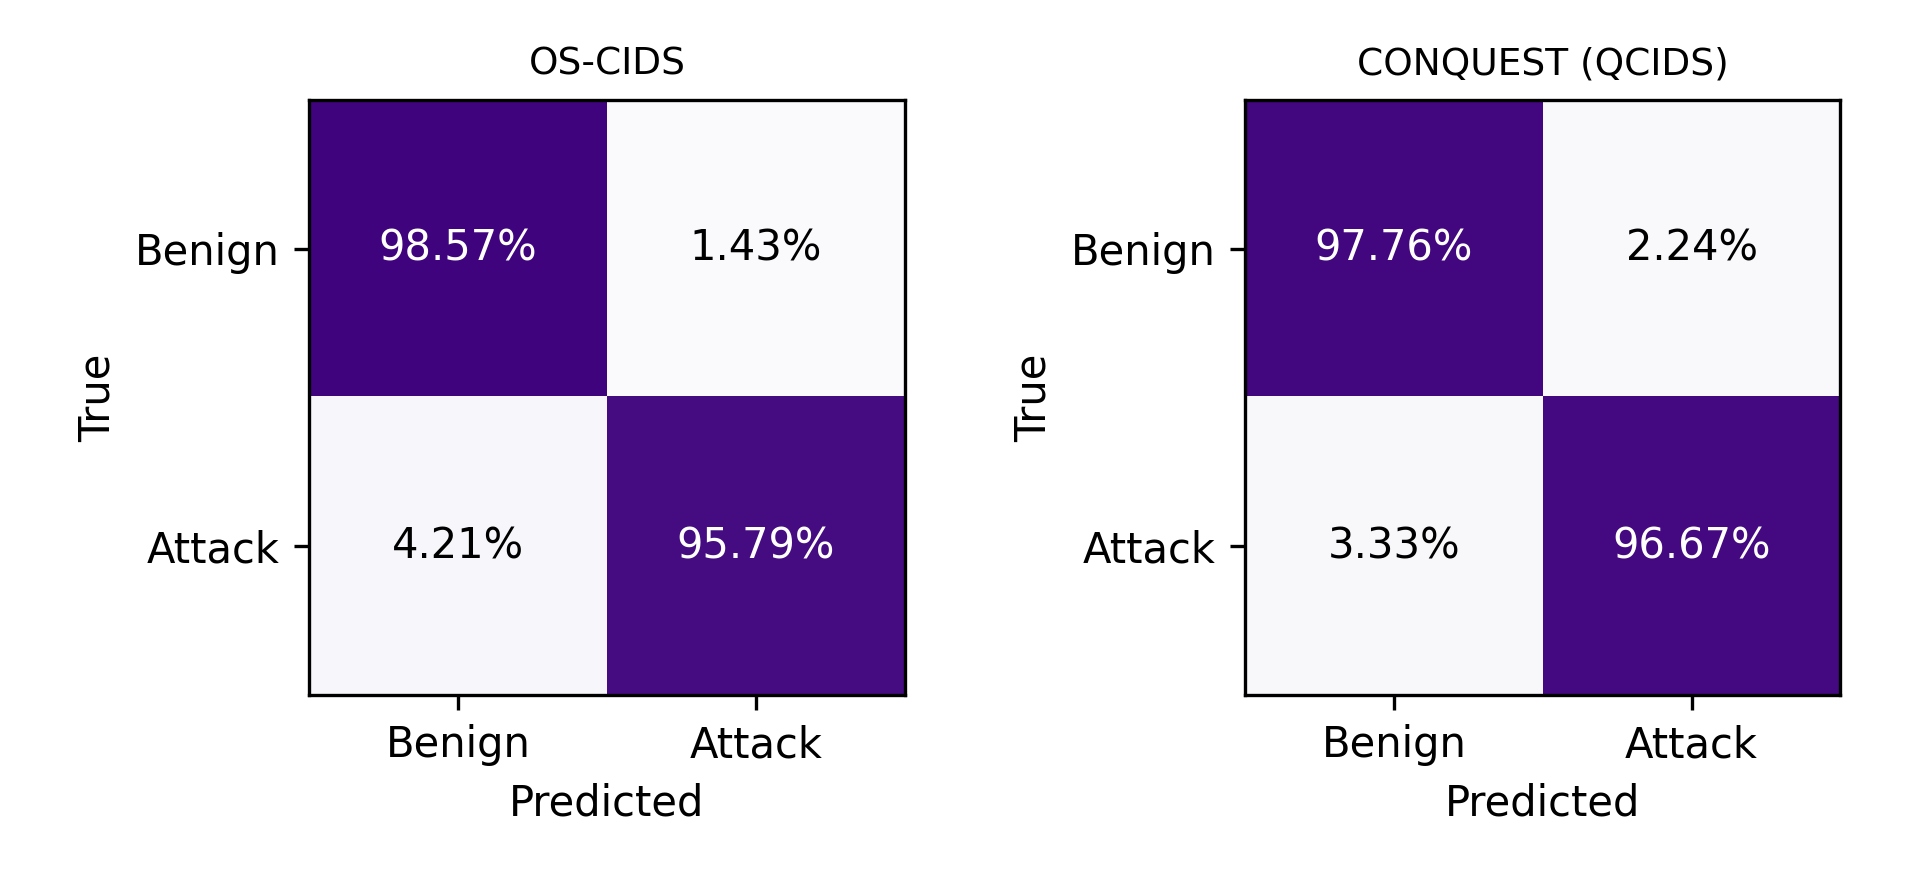
\includegraphics[width=\linewidth]{images/cm_conquest_vs_os.png}
    \caption{\textcolor{black}{Row-normalized confusion matrices of
    OS-CIDS and CONQUEST on the test set, averaged over ten seeds.}}
    
\end{figure}

\setcounter{figure}{4}
\begin{figure}[H]
    \centering
    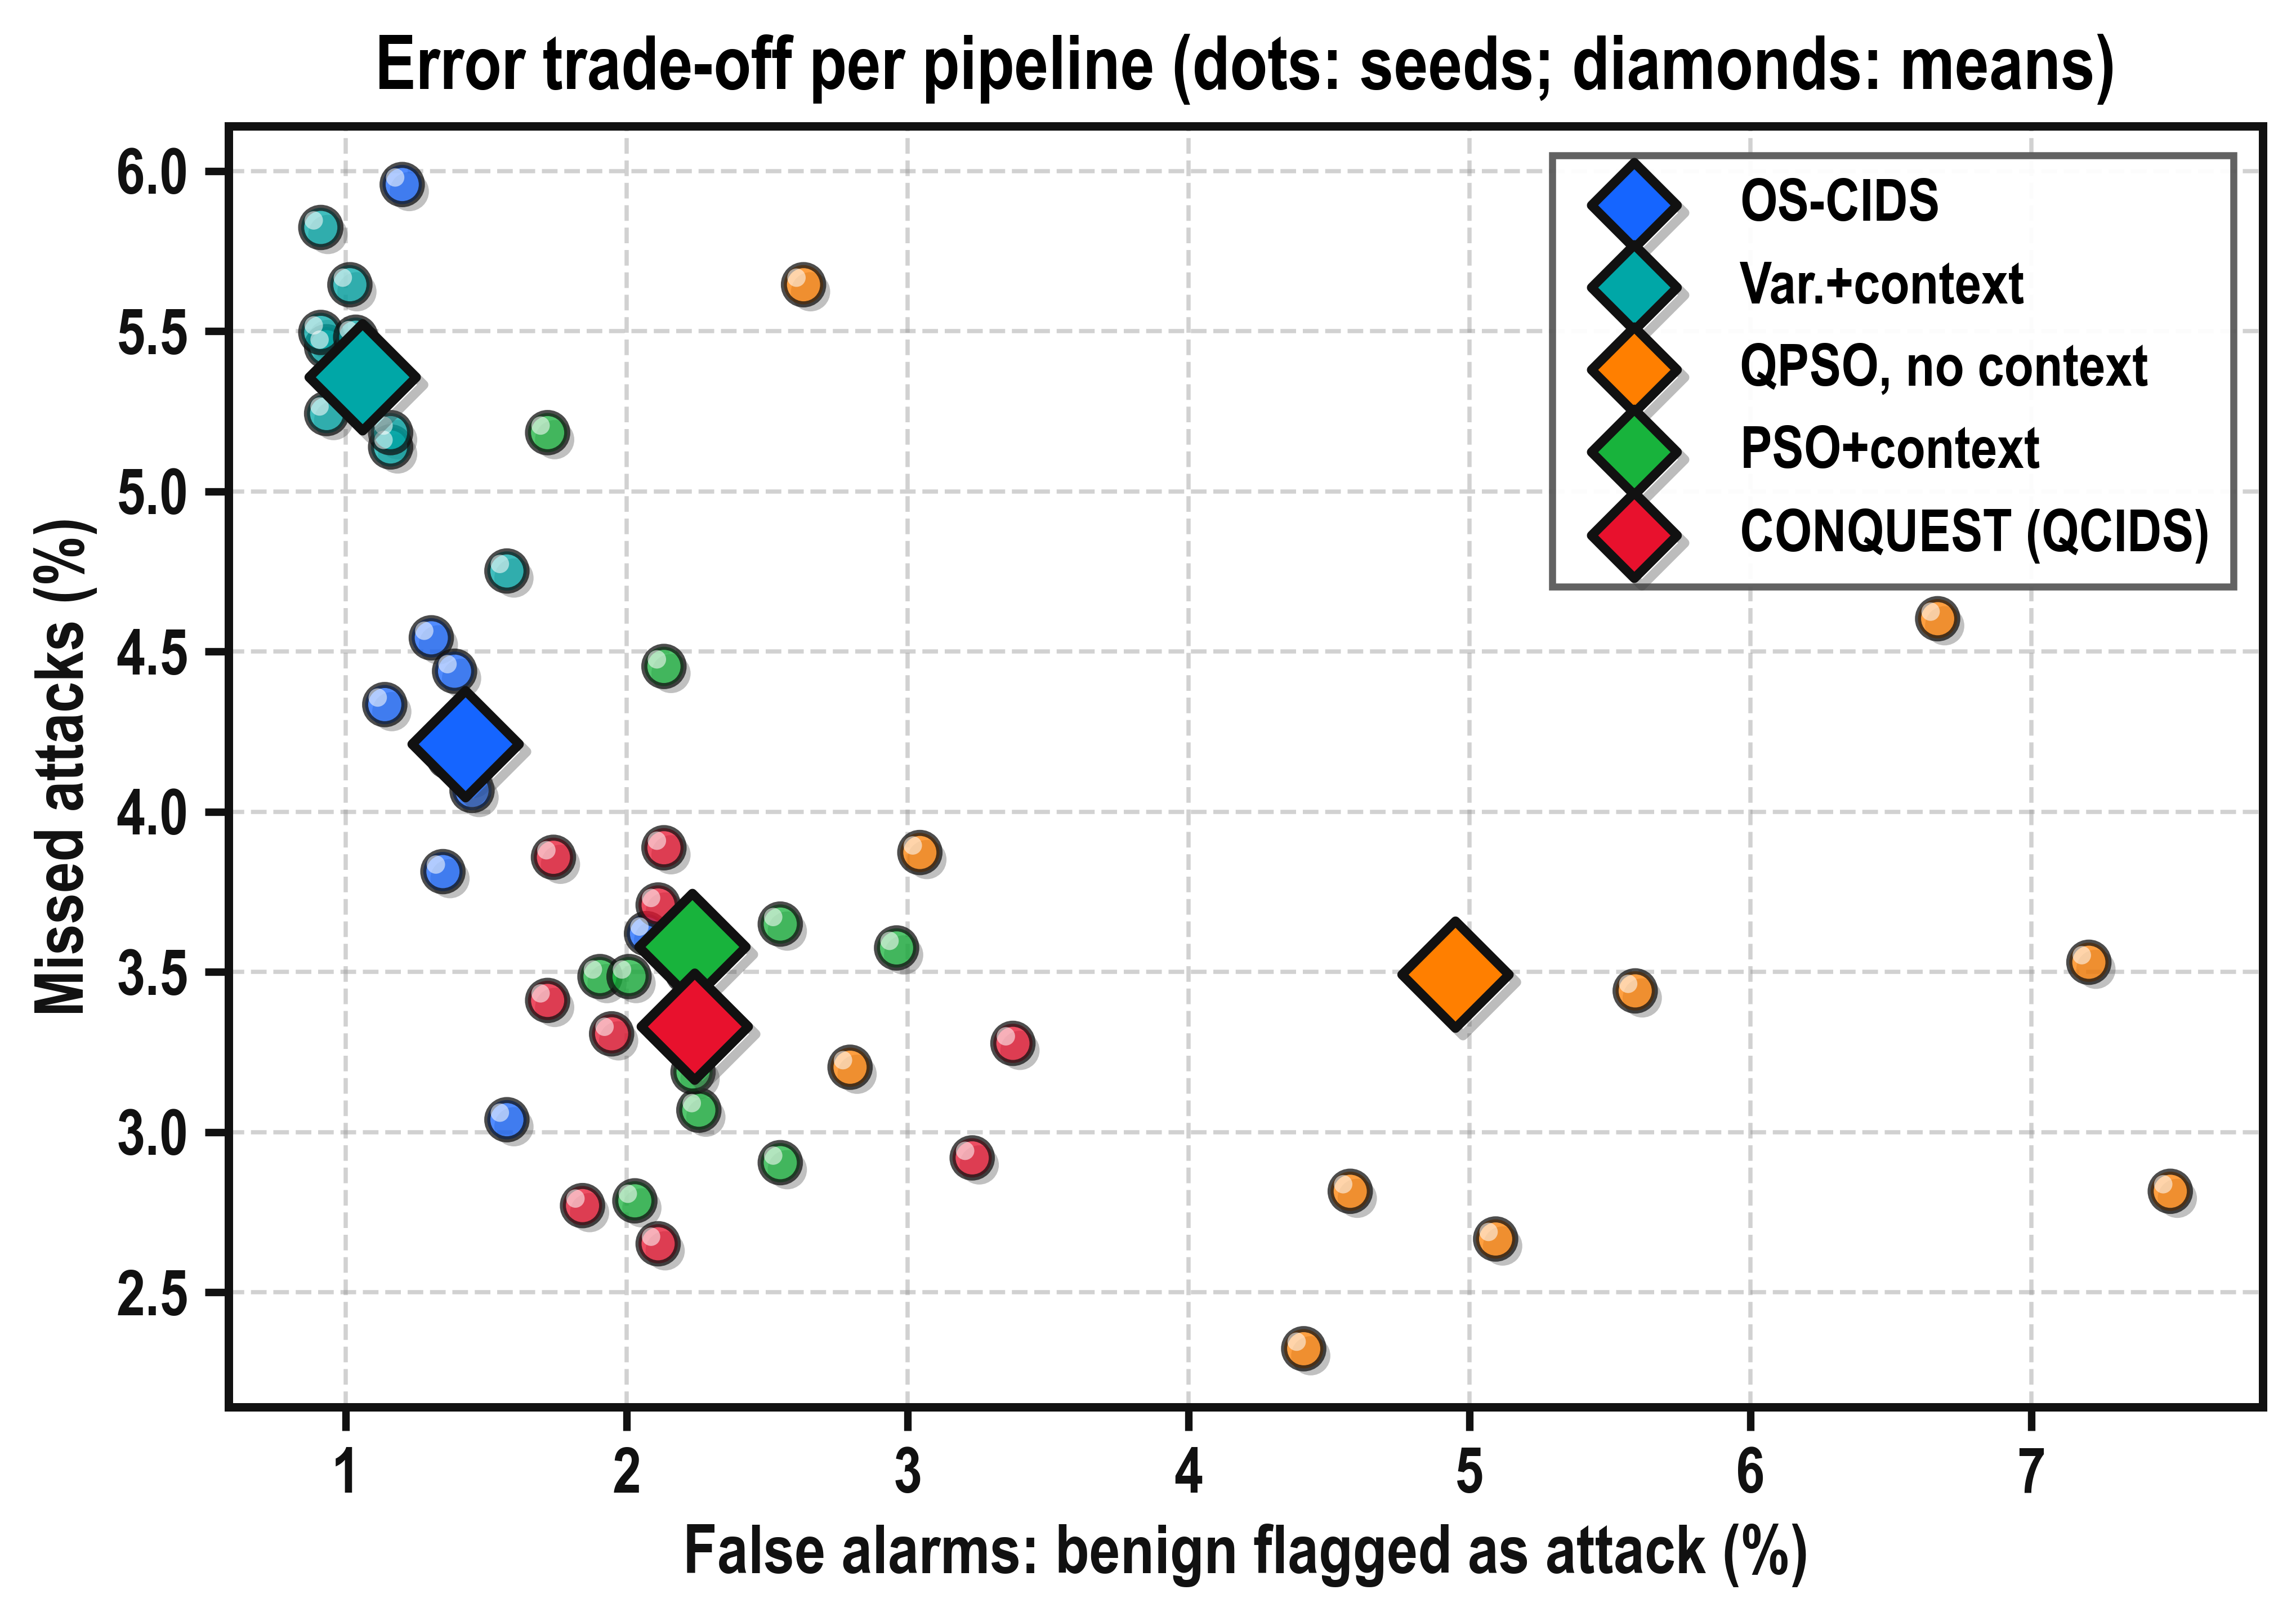
\includegraphics[width=\linewidth]{images/tradeoff_far_md.png}
    \caption{\textcolor{red}{False-alarm rate versus
    missed-attack rate of the five centralized pipelines. Dots:
    individual seeds; diamonds: means.}}
    
\end{figure}

\textcolor{black}{\textbf{Context features versus QPSO.} The
factorial ablation in Table~X separates
the two components, and neither helps on its own. Adding context
features to variance ranking lowers F1 by 0.51\,pp ($p=0.014$),
because variance ranking ignores labels and fills 14 of its 40 slots
with high-variance context counts, displacing informative
packet-length features. Replacing variance ranking by QPSO on static
features alone lowers F1 by 1.07\,pp ($p=0.002$), mainly through more
false alarms. Combined, however, context features and QPSO raise F1
by 1.23\,pp over QPSO alone and by 0.68\,pp over variance ranking with
context (both $p\le0.004$), and their interaction, $+1.74$\,pp
($p=0.002$), is the dominant effect. The gain of CONQUEST therefore
comes from combining context-aware representation with label-aware
selection, which keeps eight context features alongside complementary
static features, as listed in Table~XI.}

\setcounter{table}{9}
\begin{table}[H]
\centering
\scriptsize
\caption{\textcolor{black}{Factorial ablation of context features and QPSO over ten seeds.}}

\color{black}
\setlength{\tabcolsep}{3pt}
\begin{adjustbox}{max width=\linewidth}
\begin{tabular}{lccc}
\hline\toprule
\makecell[l]{F1 / FAR / MD\\(\%)} & \makecell{Variance\\ranking} & \makecell{QPSO\\($Q^{*}{=}6$)} & \makecell{Effect of\\QPSO (pp)} \\
\hline\toprule
Static only & 96.96 / 1.43 / 4.21 & 95.90 / 4.95 / 3.49 & \makecell{$-1.07$\\($p{=}0.002$)} \\
\makecell[l]{Static +\\context} & 96.45 / 1.06 / 5.36 & \textbf{97.13} / 2.24 / \textbf{3.33} & \makecell{$+0.68$\\($p{=}0.002$)} \\
\midrule
\makecell[l]{Effect of\\context (pp)} & \makecell{$-0.51$\\($p{=}0.014$)} & \makecell{$+1.23$\\($p{=}0.004$)} & \makecell{Interaction\\$+1.74$\\($p{=}0.002$)} \\
\hline\toprule
\end{tabular}
\end{adjustbox}
\end{table}

\setcounter{table}{10}
\begin{table}[H]
\centering
\scriptsize
\caption{\textcolor{black}{Deployed consensus mask at Q = 6; context features in italics.}}

\color{black}
\setlength{\tabcolsep}{2.5pt}
\renewcommand{\arraystretch}{1.02}
\begin{adjustbox}{max width=\linewidth}
\begin{tabular}{>{\raggedright\arraybackslash}p{3.0cm}c >{\raggedright\arraybackslash}p{3.0cm}c}
\hline\toprule
Feature & Freq. & Feature & Freq. \\
\hline\toprule
\textit{syn\_frac\_src\_60} & 1.0 & Fwd URG Flags & 0.6 \\
Fwd Packets/\allowbreak s & 0.9 & Packet Length Std & 0.6 \\
\textit{bytes\_rate\_src\_60} & 0.9 & SYN Flag Count & 0.6 \\
Fwd Packet Length Min & 0.8 & RST Flag Count & 0.6 \\
Fwd Header Length & 0.8 & PSH Flag Count & 0.6 \\
Average Packet Size & 0.8 & ACK Flag Count & 0.6 \\
Protocol & 0.7 & URG Flag Count & 0.6 \\
Fwd Packet Length Std & 0.7 & Fwd Segment Size Avg & 0.6 \\
Bwd Packet Length Min & 0.7 & Bwd Packet/\allowbreak Bulk Avg & 0.6 \\
Flow IAT Max & 0.7 & Bwd Bulk Rate Avg & 0.6 \\
Bwd IAT Max & 0.7 & Subflow Bwd Bytes & 0.6 \\
Bwd IAT Min & 0.7 & \textit{n\_flows\_src\_10} & 0.6 \\
Bwd Segment Size Avg & 0.7 & \textit{pkt\_rate\_src\_10} & 0.6 \\
\textit{n\_flows\_src\_60} & 0.7 & \textit{bytes\_rate\_src\_10} & 0.6 \\
\textit{n\_distinct\_dport\_10} & 0.7 & \textit{n\_proto\_switch\_60} & 0.6 \\
Total Length of Fwd Packet & 0.6 & Total Length of Bwd Packet & 0.5 \\
Bwd Packet Length Max & 0.6 & Fwd IAT Mean & 0.5 \\
Flow Packets/\allowbreak s & 0.6 & CWR Flag Count & 0.5 \\
Flow IAT Std & 0.6 & ECE Flag Count & 0.5 \\
Fwd IAT Std & 0.6 & Active Max & 0.5 \\
\hline\toprule
\end{tabular}
\end{adjustbox}
\end{table}

\textcolor{red}{\textbf{Quantum-inspired versus classical
search.} At an equal budget of 620 fitness evaluations, classical
binary PSO reaches a higher trace-ratio fitness than QPSO, 4919
versus 4401, in less time, 76\,s versus 106\,s, while the resulting
detectors are statistically indistinguishable ($p=0.23$ for F1 and
$p=0.49$ for MD). No quantum advantage is therefore claimed. In
CONQUEST, QPSO is one interchangeable instance of label-aware swarm
selection; its practical merits are a single interpretable control
parameter and robustness to that parameter, not superior accuracy.}
\end{excerpt}

%% ---------------------------------------------------------------------
\review{2.4}{It was mentioned that 61.2\,ms end-to-end latency was also reported, with an inference time of about 3.60\,s. The authors must specify the latency unit, whether it is per sample, per batch, or for the complete test set. The authors address the detailed reproducible measurement procedure for each metric.}

\reply We thank the reviewer for this comment and agree that the units of the
reported costs were not stated. We have re-measured every deployment cost,
stated the unit of each metric, and described how each one is measured.
\begin{itemize}[leftmargin=*,itemsep=1pt]
  \item \textit{The 3.60\,s figure} was the total time to classify the
        complete test set of about 12{,}000 windows in batches, not a
        per-sample latency; it corresponds to about 0.3\,ms per window.
  \item \textit{The 61.2\,ms figure} came from an end-to-end decomposition
        that wrongly placed the QPSO feature-selection search on the
        inference path. QPSO runs once, offline, before the classifier is
        trained, and never during detection, so this figure did not describe
        a detection latency and has been removed.
  \item \textit{Two cost categories.} Section~III-D now separates the
        \textit{offline training cost}, the QPSO search time and the
        classifier training time, both wall-clock and incurred once per
        model, from the \textit{online deployment cost}, the per-window
        latency of Eq.~(15): the context-feature update for a newly arrived
        flow plus one forward pass of the classifier. QPSO does not appear in
        the deployment cost.
\end{itemize}
Every deployment metric now states its unit, and the re-measured values of
CONQUEST are as follows (Table~XV and Fig.~9):
\begin{itemize}[leftmargin=*,itemsep=1pt]
  \item \textit{Latency}, per window of ten flows at batch size 1, in ms:
        median 2.98\,ms, 95th percentile 4.55\,ms;
  \item \textit{batched cost}, per window at batch size 64, in ms: 0.25\,ms,
        or 4{,}004 windows per second;
  \item \textit{test-set time}, the total for all 11{,}544 test windows at
        batch size 64, in s: 3.23\,s, the quantity that the former 3.60\,s
        figure reported;
  \item \textit{context-feature update}, per newly arrived flow including
        normalization and masking, in $\mu$s: 16\,$\mu$s;
  \item \textit{memory}, the peak resident set size of the inference process,
        in MB: 541\,MB, within the 1\,GB target of Eq.~(16);
  \item \textit{offline QPSO search}, per run, in min: 1.8\,min, incurred once
        before training.
\end{itemize}
\textit{Measurement procedure.} All timings use \texttt{time.perf\_counter}
on the host of Table~VI with a fixed TensorFlow thread count per process.
The classifier latency is measured at batch size 1 over 1{,}000 test windows
after 50 warm-up calls and reported as the median and 95th percentile; the
batched cost is measured at batch size 64; the context-feature update is
averaged over the test stream; and the memory is read as the peak resident
set size of the inference process. All costs are measured in isolation on
the CPU-only host and reported as medians over seeds, with the number of
seeds given in Table~XV. The costs are practically the same for every
pipeline, 2.9--3.5\,ms per window and 541--658\,MB, and for $Q=1$, 6, and 8,
which confirms that the deployment cost does not depend on $Q$ (Eq.~(1)).

\loc{(a) Page 9: Added the cost categories, the units, and the measurement procedure to Section III-D}
\begin{excerpt}
\mshead{III-D}{Latency-Aware Design and Resource Constraints}


\textcolor{red}{CONQUEST distinguishes two cost
categories, which are measured and reported separately.}

\textcolor{black}{\textcolor{red}{\textit{Offline training cost} is incurred
once per model and never on the detection path. It consists of the
QPSO search time $T_{\rm QPSO}(Q)$ and the classifier training time
$T_{\rm train}$, both measured as wall-clock time.}}

\textcolor{black}{\textcolor{red}{\textit{Online deployment cost} is incurred
for every classified window. The per-window latency is}}
\begin{equation}
\textcolor{black}{\textcolor{red}{\mathcal{L}_{\rm infer} =
\mathcal{L}_{\rm ctx} + \mathcal{L}_{\rm clf},}}
\tag{15}
\end{equation}
\textcolor{black}{\textcolor{red}{where $\mathcal{L}_{\rm ctx}$ is the
incremental context-feature update for a newly arrived flow,
including normalization and masking, and $\mathcal{L}_{\rm clf}$ is
one forward pass of the classifier.}}

\textcolor{red}{All timings use \texttt{time.perf\_counter}
on the host of Table~VI, with a fixed TensorFlow
thread count per process. The classifier latency is measured at batch
size 1 and reported as the median and 95th percentile over 1{,}000
test windows after 50 warm-up calls. Batched throughput is measured
at batch size 64. For comparison with the conference version, we also
report $T_{\rm infer}^{\rm te}$, the total time to classify all test
windows at batch size 64. The context-feature update
$\mathcal{L}_{\rm ctx}$ is averaged over the test stream and reported
per flow. Memory $\mathcal{M}$ is the peak resident set size of the
inference process. The deployment targets are}
\begin{equation}
\textcolor{red}{\mathcal{L}_{\rm infer}\le\mathcal{B}_{\rm lat},
\qquad
\mathcal{M}\le\mathcal{M}_{\max}=1\,\text{GB},}
\tag{16}
\end{equation}
\textcolor{red}{where the latency budget
$\mathcal{B}_{\rm lat}$ depends on the mission and is therefore
reported rather than fixed. The memory target reflects CPU-only
mission-edge gateways that co-host safety services}, where
computation, memory, and energy are tightly
constrained~{[38]}.
\end{excerpt}

\loc{(b) Pages 15--16: Added the re-measured deployment cost with units to Section IV-B}
\begin{excerpt}
\mshead{IV-B}{Latency-Aware Performance Under Quantum-Inspired Optimization}


\textcolor{black}{Because detection is insensitive to $Q$,
this subsection examines whether $Q$ affects deployment cost and
whether the selected operating point meets mission-edge
constraints.}

\textcolor{red}{Table~XV
and Fig.~9 report the deployment cost, measured in
isolation on the CPU-only host, for the pipelines of
Section~IV-A and for five variants of
CONQUEST: the consensus mask, register sizes $Q=1$ and 8 instead of
$Q^{*}=6$, and feature budgets $k=20$ and 10 instead of 40. Classifying one window of ten flows
takes CONQUEST a median of 2.98\,ms at batch size 1, with a 95th
percentile of 4.55\,ms. In batches of 64, a window costs 0.25\,ms, or
4{,}004 windows per second. Updating the context features,
normalizing, and masking a newly arrived flow adds 16\,$\mu$s, and the
11{,}544 test windows are classified in 3.23\,s. The inference process
peaks at 541\,MB, within the 1\,GB budget. These costs are practically
the same for every pipeline, at 2.9--3.5\,ms per window and
541--658\,MB, and for $Q=1$, 6, and 8 and $k=10$, 20, and 40, since
the classifier hardly changes with the input width, from 758k to 789k
parameters. This confirms Eq.~(1) empirically. QPSO is a
training-time cost of 1.8\,min per run on the shared host, or
0.4\,min at $k=10$, incurred once before training; the consensus mask
requires ten such runs.}
\end{excerpt}
\setcounter{table}{14}
\begin{table}[H]
\centering
\caption{\textcolor{red}{Deployment cost measured in isolation; medians over seeds, with the number of seeds in parentheses.}}

\color{red}
\setlength{\tabcolsep}{4pt}
\begin{adjustbox}{max width=\linewidth}
\begin{tabular}{lcccccccc}
\hline\toprule
\textbf{Pipeline} & \multicolumn{2}{c}{Latency (ms/window)} & Batched & Test set & Context update & Memory & Params & Selection \\
 & median & p95 & (ms/window) & (s) & ($\mu$s/flow) & (MB) & & (s) \\
\hline\toprule
OS-CIDS (3) & 2.96 & 3.69 & 0.233 & 3.30 & 5.1 & 629 & 789k & 0.0 \\
Var.+context (3) & 2.94 & 3.62 & 0.244 & 3.21 & 15.9 & 638 & 789k & 0.1 \\
PSO+context (3) & 3.02 & 3.77 & 0.244 & 3.31 & 15.9 & 658 & 789k & 76.2 \\
\textbf{CONQUEST ($Q^{*}{=}6$)} (3) & \textbf{2.98} & \textbf{4.55} & \textbf{0.250} & \textbf{3.23} & \textbf{16.2} & \textbf{541} & \textbf{789k} & \textbf{106.8} \\
CONQUEST, consensus mask (3) & 2.93 & 3.70 & 0.238 & 3.15 & 15.8 & 600 & 789k & 0.2 \\
CONQUEST, $Q{=}1$ (1) & 2.93 & 3.65 & 0.250 & 3.47 & 16.5 & 652 & 789k & 96.5 \\
CONQUEST, $Q{=}8$ (1) & 3.47 & 4.31 & 0.250 & 3.29 & 16.3 & 657 & 789k & 109.9 \\
CONQUEST, $k{=}20$ (3) & 3.19 & 4.87 & 0.260 & 3.49 & 16.4 & 650 & 768k & 43.8 \\
CONQUEST, $k{=}10$ (3) & 3.09 & 4.33 & 0.257 & 3.37 & 16.5 & 645 & 758k & 22.8 \\
\hline\toprule
\end{tabular}
\end{adjustbox}
\end{table}
\setcounter{figure}{8}
\begin{figure}[H]
\centering

\includegraphics[width=0.95\linewidth]{images/deployment_cost.png}
\caption{\textcolor{red}{Deployment cost: (a)~latency per window, (b)~batched throughput, and (c)~peak inference memory.}}

\end{figure}

%% ---------------------------------------------------------------------
\review{2.5}{The manuscript explicitly extends the previously published CONQUEST conference work. The authors must clearly distinguish these two in terms of methodological, experimental, and analytical advancement.}

\reply We thank the reviewer for this comment. Table~I in the Introduction
now itemizes the differences between the conference version and the journal
extension along the three requested dimensions. Methodologically, the
extension replaces random splitting of pooled data with a blocked temporal,
training-only protocol, defines the context features and the role of $Q$
exactly, and adds federated training with three mask-construction modes.
Experimentally, it adds a ten-seed register-size ablation, a search-budget
study, a factorial ablation, an equal-budget classical PSO baseline,
feature-subset and stability analysis, and a federated evaluation under four
heterogeneity regimes, three aggregators, and up to 20 clients. Analytically,
it adds statistical testing, an analysis of the QPSO search dynamics,
tail-aware federated metrics, measured deployment cost, and a privacy
analysis. Section~IV-D summarizes these differences again in the light of the
results.

\loc{(a) Pages 1--2: Added the distinction from the conference version to the Introduction}
\begin{excerpt}
\mshead{I}{Introduction}

The rapid digitalization of mission-critical infrastructures spanning
the Internet of Things (IoT), Internet of Vehicles (IoV), and Internet
of Drones (IoD) has expanded the attack surface of networked
systems~{[1, 2]}. AI-aided cyberworms that
adapt autonomously, propagate stealthily, and mimic legitimate
traffic render signature- and rule-based defences increasingly
ineffective~{[3]}. Where delayed or incorrect decisions can
disrupt safety, mobility, or command operations~{[4]},
robust cyberworm detection is both a security requirement and an
operational necessity.

Existing IDS approaches remain limited in this setting.
Signature-driven methods generalize poorly to novel threats, and
statistical anomaly detectors raise many false alarms under noisy,
heterogeneous traffic. Deep learning improves spatio-temporal pattern
recognition~{[5]}, but three challenges persist:
(\textit{i})~optimization degrades in high-dimensional feature spaces;
(\textit{ii})~performance is brittle under non-stationary data; and
(\textit{iii})~centralized training conflicts with the privacy,
sovereignty, and regulatory constraints of distributed missions.

Quantum-inspired optimization targets the first
challenge~{[6, 7]}: QPSO introduces
probabilistic search dynamics \textcolor{black}{that have been reported
to improve exploration over classical metaheuristics}. In IDS,
however, its use remains ad hoc: the effect of the optimizer's
configuration on its search is rarely analyzed, stability is seldom quantified, and
\textcolor{black}{comparisons with classical search at an equal
evaluation budget are missing}. Federated learning (FL) targets the
third challenge by keeping raw traffic local and exchanging only
model updates~{[8]}; \textcolor{black}{on its
own, FL provides data locality rather than formal privacy, because
updates can leak information unless secure aggregation or
differential privacy is added}. FL-based IDS studies also rarely
report worst-client behavior, convergence stability, or robustness
under realistic non-IID regimes.

This paper presents CONQUEST, a context-aware, quantum-inspired
intrusion detection framework for AI-aided cyberworm detection in
mission-critical networks. It integrates (\textit{i})~causal context
features that capture burst, dormancy, diversity, and transition cues
of cyberworm propagation; (\textit{ii})~variable-qubit QPSO for
\textcolor{black}{budget-bounded selection of a fixed-size
feature subset}; and (\textit{iii})~an LSTM(+VAE) temporal
classifier. Feature optimization runs only during training, so
deployment latency is independent of \textcolor{black}{the
QPSO register size $Q$}. This journal version extends the conference
prototype~{[9]} with an optimized non-quantum
baseline, a controlled variable-qubit ablation over
\textcolor{black}{$Q\in\{1,\dots,10\}$}, and a federated evaluation
under IID, label-skew, quantity-skew, and Dirichlet heterogeneity;
\textcolor{red}{Table~I itemizes the
methodological, experimental, and analytical differences.}
\end{excerpt}
\setcounter{table}{0}
\begin{table}[H]
\centering
\scriptsize
\caption{\textcolor{red}{Distinction between the CONQUEST conference prototype~{[9]} and this journal extension.}}

\setlength{\tabcolsep}{3pt}
\renewcommand{\arraystretch}{1.10}
\color{red}
\begin{adjustbox}{max width=\linewidth}
\begin{tabular}{p{1.5cm} p{2.4cm} p{3.9cm}}
\hline\toprule
\textbf{Aspect} & \textbf{Conference~{[9]}} & \textbf{This journal extension} \\
\hline\toprule
\multicolumn{3}{l}{\textit{Methodological}} \\
Data protocol & Random split of pooled data & Blocked temporal split; every fitting step on $\mathcal{D}_{\rm tr}$ only, as listed in Table~VII; zero-variance filter \\
Context features & Described qualitatively & 17 causal per-source features with exact definitions, windows, and dimensions in Table~IV \\
QPSO & Fixed qubit setting & Explicit role of $Q$ (Eqs.~(7)--(11), Algorithm~1); best-evaluated mask; consensus mask over seeds \\
Classifier & LSTM-VAE; optimizer comparison & LSTM(+VAE) with attention, SGD, KL-regularized latent, deterministic inference \\
Training regime & Centralized & Centralized and horizontal FL with three mask-construction modes; DP-FedAvg variant \\
\midrule
\multicolumn{3}{l}{\textit{Experimental}} \\
Baselines & Optimizer variants & OS-CIDS; context on/off $\times$ selector ablation; classical PSO at equal budget \\
Qubit study & None & $Q\in\{1,\dots,10\}$, multi-seed with per-seed QPSO; budget sensitivity up to $8\times$ evaluations \\
Feature subset & Not reported & Selected features, selection frequency, stability, consensus mask, $k\in\{10,20,40\}$ \\
FL evaluation & None & IID, label-, quantity-skew, Dirichlet; FedAvg, SCAFFOLD, FLAME; $K\in\{5,10,20\}$; privacy--utility trade-off \\
\midrule
\multicolumn{3}{l}{\textit{Analytical}} \\
Metrics & Detection rate, FPR & F1, AUC, MSE, FAR/MD, per-window latency, peak memory, $R_{99}$, $\min_k\mathrm{F1}_k$, $\sigma(\mathrm{F1})$, $\varepsilon$ \\
Statistics & Single run & Mean$\pm$std over seeds; Friedman and Holm-corrected Wilcoxon tests \\
Search analysis & None & QPSO search dynamics versus $Q$ (Fig.~3) \\
Privacy & Not analyzed & Threat model and privacy scope in Table~VIII \\
\hline\toprule
\end{tabular}
\end{adjustbox}
\end{table}

\loc{(b) Page 18: Added the advances over the conference version to Section IV-D}
\begin{excerpt}
\mshead{IV-D}{Comparison with the State of the Art and Discussion}


Table~XVII positions CONQUEST against
representative IDS and FL approaches. Because these methods are
evaluated on different datasets, a direct accuracy comparison is not
valid; the analysis instead contrasts deployment-oriented
capabilities: feature-selection stability, federated robustness,
worst-client reliability, and latency and memory compliance.
Hybrid deep-learning detectors report high accuracy on their
respective benchmarks: CNN--LSTM with
attention~{[10]} achieves up to 99.87\% on
WIoTSN, and a transformer-based IIoT
detector~{[11]} reaches 99.6\%/99.2\% Acc/F1 at
10.8\,ms inference with 37.2M parameters.
Optimization-enhanced pipelines~{[12, 13]}
exceed 99\% on NSL-KDD and UNSW-NB15. These results are
obtained under centralized assumptions with no evaluation of
optimizer stability across settings and seeds, heterogeneous client behavior,
or deployment constraints. They establish performance
ceilings on well-studied benchmarks but do not address the
reproducibility, bounded overhead, or mission-edge feasibility
requirements central to this work.

\setcounter{table}{16}
\begin{table}[H]
\centering
\scriptsize
\caption{Comparison with representative IDS and FL approaches; results come from different datasets and are not directly comparable.}

\def\rc#1{\textcolor{black}{#1}}
\setlength{\tabcolsep}{5pt}
\renewcommand{\arraystretch}{1.3}
\begin{adjustbox}{max width=\linewidth}
\begin{tabular}{>{\raggedright\arraybackslash}p{1.0cm} >{\raggedright\arraybackslash}p{2.6cm} >{\raggedright\arraybackslash}p{4.0cm} >{\raggedright\arraybackslash}p{3.2cm} >{\raggedright\arraybackslash}p{4.4cm}}
\hline\toprule
\textbf{Ref.} & \textbf{Approach} & \textbf{Key result} & \textbf{Limitation} & \textbf{Gap addressed by CONQUEST} \\
\hline\toprule
{[10]} & CNN--LSTM + attention + PSO & 98.73--99.87\% accuracy on WIoTSN; centralized & No FL, stability, or deployment analysis & \rc{Worst-client F1 of 96.4\%; 2.98\,ms per window, 541\,MB} \\
\midrule
{[11]} & Multi-scale windows + transformer + focal loss & 99.6\% accuracy, 99.2\% F1; 10.8\,ms per sample; 37.2M parameters & High complexity; no FL or resource bounds & \rc{789k parameters, 541\,MB}; FL under four heterogeneity regimes \\
\midrule
{[12]} & LPPSO + ELSTM-RNN & 99.95\% DR on NSL-KDD, 99.4\% on UNSW-NB15; centralized & No study of optimizer settings; no FL & \rc{Register-size ablation, $Q=1$ to 10}; FL under quantity and Dirichlet skew \\
\midrule
{[13]} & Ensemble + GA-PSO & Binary and multiclass accuracy gains; centralized & No temporal modeling; no FL & Context-aware temporal modeling; non-IID FL evaluation \\
\midrule
{[14]} & Federated DNN, CNN, and RNN & Up to 99.71\% on InSDN; global metrics only & Trusted aggregator; no heterogeneity tests & Four heterogeneity regimes; worst-client and dispersion metrics \\
\midrule
{[15]} & FedAvg vs.\ FedProx & 98.75\% IID, 98.44\% non-IID; two clients & No worst-client or convergence analysis & \rc{5, 10, and 20 clients}; worst-client F1 and $R_{99}$ \\
\midrule
{[16]} & Empirical FL heterogeneity study & ${\sim}$1.5K configurations; up to $4.6\times$ quality loss & General FL; not IDS-specific & Heterogeneity findings applied to cyberworm IDS \\
\midrule
{[17]} & FedAMKD & 98.83\% on MNIST; outperforms FedAvg and SCAFFOLD & Not IDS-specific; no deployment metrics & Quantity-skew analysis for IDS with tail-aware metrics \\
\midrule
{[9]} & Conference CONQUEST: QPSO + LSTM-VAE, centralized & 97.5\% DR, 0.8\% FPR on ACI-IoT; three optimizers compared & No register-size ablation, non-quantum baseline, or FL & Register-size ablation, OS-CIDS and \rc{equal-budget PSO} baselines; FL under four regimes \\
\midrule
\textbf{This work} & Context-aware preprocessing + variable-qubit QPSO + LSTM(+VAE); centralized and FL & \rc{97.13\% F1, 0.9924 AUC; 2.98\,ms per window, 541\,MB; federated: 96.66\% F1, worst client 96.4\%} & \rc{F1 on par with variance ranking and PSO; more false alarms than variance ranking} & \rc{Explicit role of the register size in the search}; unified centralized and federated evaluation with deployment metrics \\
\hline\toprule
\end{tabular}
\end{adjustbox}
\end{table}

FL-based systems~{[14, 15]}
demonstrate that \textcolor{black}{collaborative} detection is feasible
without raw data sharing, reporting global accuracy up to
99.71\% under IID conditions. However, these studies evaluate
at most two clients, report only global average metrics, and
do not quantify worst-client performance, convergence
stabilization, or behavior under realistic non-IID regimes.
Large-scale empirical analyses~{[16]}
confirm that heterogeneity can cause up to $4.6\times$ quality
degradation, while FL optimization
studies~{[17]} address quantity-skew on general
vision benchmarks without IDS-specific deployment metrics.
None of these works link non-IID robustness to
mission-facing criteria such as $R_{99}$,
$\min_k\,\mathrm{F1}_k$, or $\sigma(\mathrm{F1})$.
CONQUEST addresses the limitations of both lines of work
within a unified reproducible pipeline. Under centralized
evaluation on ACI-IoT, \textcolor{black}{CONQUEST achieves
Acc/F1/AUC\,$=$\,97.13\%/97.13\%/0.9924 with the lowest
missed-attack rate of the compared pipelines. A factorial
ablation and an equal-budget classical baseline attribute this to
the combination of context features with label-aware selection,
not to the quantum-inspired search itself, and expose a
missed-attack versus false-alarm trade-off against variance
ranking that centralized IDS studies rarely report.}
\textcolor{black}{Its deployed detector classifies a window in
2.98\,ms with 541\,MB peak memory on a CPU-only host, which
centralized IDS studies seldom measure.}
Under federated deployment,
\textcolor{black}{F1/AUC\,$=$\,0.9666/0.9914 under quantity skew, with
$R_{99}$ of 7.3 rounds, a worst-client F1 of $96.4\%$, and an
inter-client dispersion of $0.7$\,pp, show that the
centralized-federated gap stays below 0.9\,pp outside label skew}
while preserving \textcolor{black}{raw-data locality}, a trade-off that
prior FL-IDS work neither quantifies nor justifies
experimentally.

The conference prototype~{[9]} reported
97.5\% detection rate and 0.8\% FPR on ACI-IoT under
centralized evaluation, establishing the first
cyberworm-focused CONQUEST result. \textcolor{red}{The
two works differ in method, experiments, and analysis,
as Table~I summarizes. Methodologically, the extension
replaces random splitting of pooled data with a blocked temporal,
training-only protocol, defines the context features and the role
of $Q$ exactly, and adds federated training. Experimentally and
analytically,} the journal extension
advances this in three ways: (i)~a
variable-qubit analysis over $Q=1$ to 10
that \textcolor{black}{makes the role of $Q$ explicit and
characterizes its effect on search dynamics and detection}
\textcolor{black}{and shows that detection is statistically
insensitive to $Q$, so the operating point is set by a pre-declared
validation rule}; (ii)~\textcolor{black}{a factorial ablation
and an equal-budget classical PSO baseline that attribute the
detection gain to the combination of context features and
label-aware selection rather than to quantum-inspired search};
and (iii)~federated
evaluation under four heterogeneity regimes with
mission-facing deployability metrics that prior
QPSO-based IDS work does not provide. Together, these
extensions transform a centralized feasibility demonstration
into a deployment-oriented framework with quantified
robustness bounds.
\end{excerpt}

\bigskip
\noindent\textbf{Overall, the authors wish to thank the editor and all the
reviewers for their insightful review comments and constructive criticisms,
which have helped the authors improve the quality of the revised manuscript
in terms of content and clarity.}

\end{document}
